% !TeX program = pdflatex
\documentclass[a4paper,english]{article}
\usepackage[utf8]{inputenc}
%\usepackage[T1]{fontenc} % to use the accented characters as individual glyphs
						  % automatically hyphenate words for European 
						  % languages (German, French, Italian, etc.)
\usepackage[USenglish]{babel}
\usepackage[none]{hyphenat}
\usepackage[margin=1in]{geometry}
\usepackage{enumerate}
\usepackage{amsmath}
\usepackage{amssymb}
\usepackage{amsfonts}
\usepackage{mathtools}
\DeclarePairedDelimiter\norm{\lVert}{\rVert}
\newcommand{\vertiii}[1]{{\left\vert\kern-0.4ex\left\vert\kern-0.4ex\left\vert
	#1 \right\vert\kern-0.4ex\right\vert\kern-0.4ex\right\vert}}
\usepackage{bm}
\usepackage{cases}
\usepackage{esvect}
\usepackage{amsthm}
\newtheorem{theorem}{Theorem}[section]
\newtheorem{lemma}[theorem]{Lemma}
\newtheorem{corollary}[theorem]{Corollary}
\theoremstyle{definition}
\newtheorem{definition}{Definition}[section]
\theoremstyle{remark}
\newtheorem{remark}{Remark}
\renewcommand\qedsymbol{$\square$}

\usepackage[framemethod=TikZ]{mdframed} % to create elegant boxes, frames
\mdfdefinestyle{mdftheoremstyle}{
	linecolor=green,linewidth=1pt,roundcorner=10pt,
	frametitlerule=true, frametitlerulewidth=.5pt,
	frametitlebackgroundcolor=green!20,
	innertopmargin=\topskip,
}
\mdfdefinestyle{mdfdefinitionstyle}{
	linecolor=blue,linewidth=1pt,roundcorner=10pt,
	frametitlerule=true, frametitlerulewidth=.5pt,
	frametitlebackgroundcolor=blue!20,
	innertopmargin=\topskip,
}
\mdtheorem[style=mdfdefinitionstyle]{mdfdef}{Definition}[section]
\mdtheorem[style=mdftheoremstyle]{mdfthm}{Theorem}[section]
\mdtheorem[style=mdftheoremstyle]{mdflma}{Lemma}[section]
%% NOTE %%
% To be consistent, choose either mdf[def,thm,lma] or the standard ones
% DON'T MIX THEM


\usepackage{standalone}  % to compile alone for efficiency
%\usepackage{afterpage}  % used when adding the cover page
%\usepackage{pdfpages}   % for inclusion of external multi-page PDF
\usepackage{xcolor}
\usepackage{colortbl}

% some user-defined colors
\definecolor{codegray}{rgb}{0.5,0.5,0.5}
\definecolor{background-color}{rgb}{0.95,0.95,0.92}
\definecolor{brilliant-blue}{RGB}{0, 176, 220}
\definecolor{mid-green}{RGB}{0,167,0}


\usepackage{graphicx}
\usepackage{subfig}
\usepackage{wrapfig}
\usepackage[justification=raggedright] % prevents spiltting words with hyphens
			{caption}
%\usepackage{pgfplots} % includes tikz
\usepackage{tikz}
\usetikzlibrary{shapes.geometric,calc,matrix,hobby}
\newcommand*\circled[1]{\tikz[baseline=(char.base)]{
	\node[shape=circle,text=white,fill=black,inner sep=.5pt] (char) {#1};}}	
\newcommand*\orangecircled[1]{\tikz[baseline=(char.base)]{
	\node[shape=circle,fill=orange,inner sep=.5pt] (char) {#1};}}
\newcommand*\greencircled[1]{\tikz[baseline=(char.base)]{
	\node[shape=circle,text=white,fill=mid-green,inner sep=.5pt] (char) {#1};}}
\newcommand\greencircle{\tikz[baseline=(char.base)] 			
	\node[fill=mid-green,circle]{};}
\usepackage{tkz-euclide} % \tkzMarkAngle


\usepackage{algorithm}
%\usepackage{algorithmicx} % automatically loaded by `algpseudocode`
\usepackage{algpseudocode} % layout for algorithmicx

\usepackage[toc,page]{appendix}
%\usepackage[square,numbers]{natbib}
%\bibliographystyle{abbrvnat}

% configuration of biblatex with biber:
%https://tex.stackexchange.com/questions/154751/biblatex-with-biber-configuring-my-editor-to-avoid-undefined-citations
\usepackage[
backend=biber,
style=alphabetic,
sorting=ynt
]{biblatex}
\addbibresource{bibliography.bib}


\usepackage[newfloat]{minted} % compile with -shell-escape flag
% outputdir=./tmp causes problems, since \minted still looks for 
% temporary files in the document root directory.

%\renewcommand{\listingscaption}{Code}% only applies when newfloat is unset
\renewcommand*\listingname{Code listing}

% minted lineno style
\renewcommand{\theFancyVerbLine}{\sffamily
	\textcolor{codegray}{\tiny
		%		\scriptsize% \oldstylenums
		{\arabic{FancyVerbLine}}}}
\setminted{
	mathescape=true,
%	escapeinside=||,
	linenos=true,
	numbersep=1.5mm,
	autogobble,
	breaklines,	breakanywhere,
	fontsize=\footnotesize,
	style=xcode,
	bgcolor=background-color
}
% Create a new environment for breaking code listings across pages.
\newenvironment{code}{\captionsetup{type=listing}}{}


\usepackage{fancyhdr}
\pagestyle{fancy}
\fancyhf{} 	% clears the header and footer of default "plain" page style
\lhead{\leftmark}
\rhead{\thepage}
\chead{\hyperlink{Contents}{Contents}}

\usepackage{hyperref, bookmark}

\hypersetup{
	pdftitle = {FEM2d},
	pdfsubject = {Numerical Analysis},
	pdfkeywords = {Finite Element Methods},
	pdfauthor = {Mark Taylor},
	bookmarks = true,
	bookmarksnumbered = true,
	pdfpagelabels = true,
	pdfpagemode = UseOutlines,
	pdfstartview = FitH,
	linktocpage = true,
	colorlinks = true,
	citecolor = orange, 
	linkcolor = brilliant-blue,
	urlcolor = magenta,
	plainpages = false
}

\setcounter{section}{-1}
\linespread{1.1}

% vertical space for tabular before/after \hline
\newcommand\Tstrut{\rule{0pt}{3.0ex}}         % = `top' strut
\newcommand\Bstrut{\rule[-1.5ex]{0pt}{0pt}}   % = `bottom' strut
\newcommand\grad{\mathbf{grad}\,}
\newcommand{\bx}{\bm{x}}
\newcommand{\rd}{\mathrm{d}}
\newcommand{\dx}{\rd\bx}
\newcommand{\bA}{\mathbf{A}}
\newcommand{\ba}{\bm{a}}
\newcommand{\inangle}[1]{\langle #1 \rangle}

\def\Plus{\texttt{+}}
\def\Minus{\texttt{-}}




\begin{document}	
	\title{
		{The Standard Finite Element Method and the Weak Galerkin Method for 
			Elliptic Boundary Value Problems}\\
		\textbf{{\Large Senior Thesis}}\\[1cm]
	
		\textit{{\Large written by}}\\
		{{\Large Mark Taylor}}\\[1cm]
		
		\textit{{\Large supervised by}}\\
		{\Large Prof. Qilong Zhai}\\
		
		{\Large Department of Mathematics}\\
		{\Large Jilin University}
	}	
	\date{\today}
	\pagenumbering{roman}
	\maketitle
	\thispagestyle{empty}
	
	\begin{abstract}
		\normalsize		
		This thesis introduces the bare-bones of finite element methods (FEM)
		for second-order elliptic boundary value problems and presents a
		straightforward implementation in MATLAB for the standard FEM. Then 
		We give some conclusions about error estimates and the rate of 
		convergence. In the end, we provide a cutting-edge 
		technique---the weak Galerkin method as a comparison to the 
		standard (Galerkin) FEM. The accuracy of approximation by these two
		methods will be analyzed experimentally through a couple of numerical 
		experiments.
	\end{abstract}
	
	\clearpage
	\section*{Acknowledgment}
	First, the author would like to thank Prof. Ralf Hiptmair who wrote (and 
	is actively updating) 
	\href{https://www.sam.math.ethz.ch/~grsam/NUMPDEFL/NUMPDE.pdf}{this} 
	MARVELOUS FEM (NPDE actually) book. It is of extremely high quality, 
	comprising a tremendous number of beautiful figures which makes the book 
	incredibly accessible and interesting. %Highly recommended! 
	
	Then the author	want to thank Prof. Qilong Zhai who has provided great 
	suggestions in the writing and for supervising the author with great
	patience and responsibility. This thesis couldn't be done without his help.
	
	In addition, the author is extremely grateful to Miss White for discussing 
	the quadratic finite elements for the two-point boundary value problems 
	with him last term, which underlay an important understanding of higher 
	order finite elements to the author. Also, the author is very appreciative
	of the practical help from Shuaishuai Lu in implementing FEM.
	
	Lastly, the author want to give thanks to my awesome roomies who have been 
	there for me sharing joys and sorrows with me in these years, to all the 
	adorable classmates and cute teachers who have made our college life this 
	lovely, and most of all huge thanks to my beloved parents who have always 
	been so supportive.
	\thispagestyle{empty}
	
	\clearpage
	\hypertarget{Contents}{}  % Make an anchor to the toc
%	\phantomsection  % optional
	\pdfbookmark[1]{\contentsname}{Contents}    % at current level (== 1)
%	\belowpdfbookmark{\contentsname}{Contents}  % equivalent to above one	
	\tableofcontents
	
	\listofalgorithms
	\addtocontents{loa}{\def\string\figurename{Algorithm}}
	
	
	\clearpage
	\pagenumbering{arabic}
	\section{Introduction}
%	\subsection{Background}
%	Blah, blah,... to be added
%	The finite element method (FEM) originated from the need to solve complex 
%	elastic and structural analysis problems in civil and aeronautical 
%	engineering, and introduced in the late 1950s in the aircraft industry. 
%	Use of the techniques followed a paper 
%	by Turner, Clough, Martin, and Topp \cite{TCMT} that was published in 
%	1956. Wide spread application of the methods required large computer
%	recourses that were not available until the early 1970s.\cite{NA9e}\quad
%	And now the finite element method has emerged as one of the most 
%	powerful and widely used numerical methods for solving partial differential
%	equations (PDEs) arising in engineering and mathematical modeling. 
%	Typical problem areas of interest encompass the traditional fields of
%	structural analysis, heat transfer, fluid flow, mass transport, and 
%	electromagnetic potential.
%	
%	When compared to other numerical methods, for example,
%	the finite difference method (FDM),
%	FEM has a couple of proven advantages over FDM.  The most attractive and
%	desirable feature of FEM is its ability to handle complicated geometries
%	and boundaries with relative ease, whereas the FDM in its basic form is 
%	restricted to handle regular rectangular shapes.
%	In fact, many real-world
%	physical problems have boundary conditions involving derivatives and 
%	irregularly shaped boundaries. Boundary conditions of this type are 
%	difficult to handle using finite-difference techniques because each 
%	boundary condition involving a derivative must be approximated by a 
%	difference quotient at the grid points, and irregular shaping of the 
%	boundary makes placing the grid points difficult. The finite element 
%	method includes the boundary conditions as integrals in a functional 
%	that is being minimized, so the construction procedure is independent
%	of 	the particular boundary conditions of the problem.\cite{NA9e}\quad	
%	Besides, the quality (accuracy) of a FEM approximation is, in general,
%	higher than its counterpart in FDM.
%	
%	Notwithstanding the difficulties in its implementation, quite
%	a number of excellent (open-source) FEM libraries have been implemented,
%	and now the techniques have matured considerably after decades
%	of efforts. These feature-rich software have been
%	used extensively both in academia and industry.
%	Among them, a few noted are
%	\href{https://dealii.org}{deal.II}, 
%	\href{http://libmesh.github.io/}{libMesh},
%	\href{https://fenicsproject.org/}{FEniCS},
%	\href{http://www.elmerfem.org/blog/}{Elmer FEM},
%	\href{https://mfem.org}{MFEM},
%	\href{https://freefem.org/}{FreeFEM},
%	and among which the 
%	\href{https://dealii.org}{deal.II} library is the most comprehensive,
%	the most well documented, and is one the most well-established,
%	state-of-the-art, and actively-maintained FEM libraries.
%	If you are about to implement your own finite element library, 
%	the \href{https://dealii.org}{deal.II} library is definitely 
%	a superb go-to reference that can help you quickly understand the
%	main framework and essentials of a FEM library.
	
%	\subsection{Contents and Organization of This Thesis}	
	This thesis consists of two parts: Section \ref{section.1}--\ref{section.5}
	is the first part introducing the standard Galerkin FEM, and Section
	\ref{section.6} is the second part introducing the weak Galerkin FEM.
	
	In the first part, we extract and summarize the essentials 
	(weak formulation, discretization, and implementation details)
	of finite element methods in the online book
	\textit{Numerical Methods for Partial Differential Equations} 
	\cite{Hiptmair} from ETH Lecture
	\href{https://video.ethz.ch/lectures/d-math/2018/spring/401-0674-00L.html}
	{401-0674-00L} by Prof. Ralf Hiptmair. We will also add some our own 
	understanding in it, of course. We aim to make it as accessible as possible.
	So We present this part in a way such that one can learn by analogy. This 
	is made easy by first examining the one-dimensional two-point boundary
	value problems. Then by analogy one can smoothly proceed to the 
	two-dimensional	elliptic boundary value problem. It allows one to learn
	the basic concepts of FEM with relative ease.
	By learning this five sections one can implement a small framework for 
	numerically solving some elliptic boundary values problems in the 
	standard Galerkin FEM. We also provide a minimum implementation in 
	MATLAB, the code of which can be found at 
	\url{https://github.com/How-u-doing/Numerical_Analysis/tree/master/%
		Chapter11_FEM2d}. 
	Besides, the 1D counterpart involved in Section
	\hyperref[subsection.5.3]{5.3} is available at
	\url{https://github.com/How-u-doing/Numerical_Analysis/tree/master/%
		Chapter10_BVPforODEs}.
		
	We start our journey in Section \hyperref[section.1]{1} by converting 
	boundary value problems into their equivalent weak formulations. 
	In the second part, Section \hyperref[section.2]{2},
	we provide the discretization of boundary value problems, which
	is only one, but a critical step in numerical treatment of boundary
	value problems. This step assembles and builds the Galerkin matrix and
	right-hand side vector, which are the two final components in finite
	element methods that will then be used to solve the linear systems of
	equations in order to obtain the numerical solution.
	Also, the assembly of mass matrix and the imposition of natural and 
	essential boundary conditions will be discussed.	
	Subsequently, by convention, we ``analyze" the accuracy and convergence 
	of this numerical method (FEM) in Section \hyperref[section.3]{3}.	
	The fourth segment in Section \hyperref[section.4]{4} contains some
	implementation details in the context of MATLAB, including mesh generation, 
	index mapping, local computations of element matrices and element vectors,
	incorporation of boundary conditions, etc. To the end of the first part,
	we present two numerical experiments of 2nd-order elliptic boundary value 
	problems in Section \hyperref[section.5]{5}. We will solve those two BVPs 
	using the algorithms mentioned in Section \hyperref[section.2]{2} and 
	Section \hyperref[section.4]{4}. Additionally, examples of 
	two-point BVPs that	employ both linear finite elements and quadratic 
	finite elements are	also provided for the sake of comparison and 
	completeness.
	
	In the end, in the second part as a further reading, we	provide and discuss 
	a newly developed novel technique, the weak Galerkin finite element	method.
	The introduction of the weak gradients makes it powerful enough to handle 
	non-continuous piecewise polynomial across cells. We will see how it 
	differs from the standard Galerkin FEM in terms of approximation quality in 
	Section \ref{subsection.6.4}.
	
	\clearpage
	\section{Weak Formulation}\label{section.1}
	A finite element method is characterized by a variational formulation,
	a discretization strategy, one or more solution algorithms, 
	and post-processing procedures. In this section, we will transform our 
	mathematical models (boundary value problems) into their corresponding  
	weak formulations. Let us first look at two model problems that
	will form the basis for this thesis.
	
	\hypertarget{P1}{P1}:
	 A one-dimensional two-point boundary value problem
	 with homogeneous Dirichlet boundary conditions
	\begin{align}
	  -\frac{\rd}{\rd x}\left(p(x)\frac{\rd u}{\rd x}\right)+q(x)u&=f(x),
	   \quad x\in (a,b), \label{eq:ODE model}\\
	 u(a) &= 0,\ u(b) = 0, \label{eq:ODE Dir BCs}
	\end{align}
	where $p(x) \in C^1(\bar{I}),\; p(x)\geq p_{min}>0,\; 
	q(x) \in  C^1(\bar{I}),\; q(x)\geq 0,\; f(x) \in L^2(I),\;
	I =\,]a,b[ $.\footnote{The notation $]a,b[$ is used for an open 
	interval, more commonly written as $(a,b)$. But the latter can be
	confused with a vector or an element of $\mathbb{R}^2$. } \\	
	
	
	\hypertarget{P2}{P2}:
	 A second-order elliptic homogeneous Neumann problem
	\begin{align}
	-\nabla\cdot(\bm{\alpha}(\bx) \nabla u)+
	\gamma(\bx)u=f,\quad &\textrm{in} \ \Omega,
	\label{eq:PDE model} \\ 
	\bm{\alpha}(\bx)\nabla{u}\cdot\bm{n}=0,\quad &\textrm{on}\ \partial\Omega,
	\label{eq:PDE Neu BC}
	\end{align}
	where $\Omega$ is an open bounded domain in $\mathbb{R}^2$,
	$\nabla{u}$ denotes the gradient of the function $u$, 
	$\bm{\alpha}$ is a symmetric uniformly positive definite\footnote{
		A matrix-valued function $\bA:\Omega\mapsto\mathbb{R}^{n,n},n\in
	\mathbb{N}$, is called uniformly positive definite, if
	\[\exists\epsilon^{-}>0:\quad\bm{z}^\top\bA(\bx)\bm{z}\geq 
	\epsilon^{-}\norm{\bm{z}}\quad\forall\bm{z}\in\mathbb{R}^{n}\]
	for \emph{almost all} $\bx\in\Omega$, that is, only with the exception of
	a set of volume zero.
	}
	$2\times 2$	matrix-valued function, $\gamma$ is a scalar-valued 
	function, and $\bm{n}$ is the outward unit vector normal to the 
	boundary $\partial \Omega$.\\
	
	
	For differential equation \eqref{eq:ODE model} in \hyperlink{P1}{P1}, 
	multiplying a test function $v(x)$ on both sides and applying 
	integration by parts we have
	\begin{align}
	\int_a^b\left[-\frac{\rd}{\rd x}\left(p(x)\frac{\rd u}{\rd x}\right)v
		+q(x)uv\right] \rd x &= 
	\int_a^b\left(p(x)\frac{\rd u}{\rd x}\frac{\rd v}{\rd x}+q(x)uv\right)\rd x
		-p(x)\frac{\rd u}{\rd x}v(x)|_a^b \label{eq:ODE int by parts}\\
						  &=\int_a^b fv\, \rd x. \nonumber	
	\end{align}	
	Now we choose the test space  
	$V=H_0^1:=\{u\in H^1(I)$,\footnote{ $H^1(\Omega)$ is a the
		Sobolev space of functions on $\Omega$
		with generalized derivatives $L^2(\Omega)$, i.e.
	\[ H^1(\Omega) := \{v:\Omega\mapsto\mathbb{R}\; \textrm{integrable}:\ 
	\int_{\Omega}|\nabla v(\bx)|^2 \dx < \infty \} \] }
	$u=0\textrm{ at }x=a \textrm{ and } x=b\}$ and $v(x)\in V$,
	then the second term on the right-hand side of \eqref{eq:ODE int by parts}
	vanishes since $v(a)=v(b)=0$. Hence,	
	\begin{equation} \label{eq:ODE int result}
	\int_a^b\left(p(x)\frac{\rd u}{\rd x}\frac{\rd v}{\rd x}+q(x)uv\right)\rd x	
	 	= \int_a^b fv\, \rd x	\quad \forall v\in V.
	\end{equation}
	Using space of trial functions $U=V$ we can rephrase problem 
	\eqref{eq:ODE int result} in the following \emph{weak} form:
	\begin{equation}\label{eq:weak form}
	\begin{cases}
	\textrm{Find}\ u\in U \ \textrm{such that}\\
	 	a(u,v)=\ell(v) \quad \forall v\in V.
	\end{cases}
	\end{equation}		
	Here $a : U \times V \mapsto \mathbb{R}$ is a continuous bilinear
	form and $\ell : V \mapsto \mathbb{R}$ is a continuous linear form,
	with
	\begin{equation}
	a(u,v)=\int_a^b\left(p(x)\frac{\rd u}{\rd x}\frac{\rd v}{\rd x}+
		q(x)uv\right)\rd x, \quad \ell(v)=\int_a^b fv\, \rd x.
	\end{equation}
	Problem \eqref{eq:weak form} is also referred to as a  
	\emph{variational problem} and as the \emph{variational form} of 
	(\ref{eq:ODE model},~\ref{eq:ODE Dir BCs}). The reasons for using the terms
	``variational" and ``weak" to describe \eqref{eq:weak form} are explained
	in \cite{UIFEM}.\\	
	
	The standard finite element approximation of \eqref{eq:ODE int result} 
	amounts to the construction of Galerkin or weighted residual 
	approximations of (\ref{eq:ODE model},~\ref{eq:ODE Dir BCs}) over 
	% The tilde above serves as a unbreakable space
	\emph{finite dimensional} subspaces $U_h \subset U$ and 
	$V_h \subset V$.\footnote{The subscript $h$ is a discretization parameter 
	generally chosen as a measure of the mesh size.} That is, 
	\begin{equation}\label{eq:discrete weak form}
	\begin{cases}
	\textrm{Find}\ u_h\in U_h \ \textrm{such that}\\
	a(u_h,v_h)=\ell(v) \quad \forall v_h\in V_h,
	\end{cases}
	\end{equation}
	where 
	\begin{equation}\label{eq:discrete ODE formulas}
	a(u_h,v_h)=\int_a^b\left(p(x)\frac{\rd u_h}{\rd x}\frac{\rd v_h}{\rd x}
		+q(x)u_hv_h\right)\rd x,
	\quad \ell(v)=\int_a^b fv_h\,\rd x.
	\end{equation}\\
	
	Similarly, for partial differential equation \eqref{eq:PDE model} in 
	\hyperlink{P2}{P2} we integrate by parts via Green's theorem 
	noticing the boundary condition \eqref{eq:PDE Neu BC}:
	\begin{equation*}
	\int_{\Omega}\left(-\nabla\cdot(\bm{\alpha}(\bx)\nabla u)\,v
		+\gamma(\bx)uv\right) \dx =	
	\int_{\Omega}\left(\bm{\alpha}(\bx) \nabla u \cdot \nabla v
		+\gamma(\bx)uv\right) \dx -
	\int_{\partial\Omega}\bm{\alpha}(\bx)\nabla u\cdot\bm{n}\,v\,\rd s 
	=\int_{\Omega}fv\,\dx,
	\end{equation*}
	$$\Downarrow$$
	\begin{equation}\label{eq:PDE int result}
	\int_{\Omega}\left(\bm{\alpha}(\bx)\nabla u\cdot\nabla v
		+\gamma(\bx)uv\right) \dx = \int_{\Omega}fv\,\dx\quad\forall v\in V,
	\end{equation}
	where $V=H^1(\Omega)$.
	
	Likewise, using $U=V=H^1(\Omega),\,U_h \subset U,\,V_h \subset V$
	we can obtain exactly the same \emph{discrete weak form} as that of
	\eqref{eq:discrete weak form}, but with $a(u_h,v_h)$ and $\ell(v_h)$
	being
	\begin{equation}\label{eq:discrete PDE formulas}
	a(u_h,v_h)=\int_{\Omega}\left(\bm{\alpha}(\bx)\nabla u_h\cdot\nabla v_h 
		+\gamma(\bx)u_hv_h\right) \dx,\quad\ell(v_h)=\int_{\Omega}fv_h\,\dx.
	\end{equation}
	
	(\ref{eq:discrete weak form},~\ref{eq:discrete ODE formulas}) and 
	(\ref{eq:discrete weak form},~\ref{eq:discrete PDE formulas}) are the
	\emph{discrete weak formulations} based on which we will develop our
	numerical solutions in later sections.
	
	
	\section{Discretization} \label{section.2}
	In previous section, we have derived the continuous and discrete
	weak formulations equivalent to the boundary value problems
	\hyperlink{P1}{P1}, \hyperlink{P2}{P2}. Reducing the continuous 
	infinite dimensional problems to a finite dimensional vector subspace 
	allows us to numerically compute $u_h$ as a finite linear combination
	of the basis vectors in $U_h$. In this section we will
	dive into the details of Galerkin discretization, which consist of three
	parts: choice of trial/test space, choice of basis, computing Galerkin 
	matrices and right-hand side vectors.	
		 
	\subsection{Choices of Trial/Test Space and Basis}\label{subsection.2.1}
	We adopt Galerkin method throughout this thesis so we have
	$U_h=V_h$ (in general, $U_h\neq V_h$, though).
	Let $\mathfrak{B}_h=\{b_h^1, b_h^2, ..., b_h^N \}$	be an ordered
	basis of $U_h$, then $u_h,\,v_h$ can be written as follows
	\begin{align}
	u_h&=\mu_1 b_h^1+\mu_2 b_h^2+...+\mu_N b_h^N, \quad\mu_i\in\mathbb{R},
	\label{eq:linear combi of u_h}\\	
	v_h&=\nu_1 b_h^1\,+\nu_2 b_h^2\,+...+\nu_N b_h^N,\,\quad\nu_i\in\mathbb{R}.
	\label{eq:linear combi of v_h}	
	\end{align}
	The number $N\in \mathbb{R}$ above is the dimension of the discrete
	trial and test space $U_h$, i.e. $N:=\mathrm{dim}\,U_h$.	
	
	Inserting \eqref{eq:linear combi of u_h} and \eqref{eq:linear combi of v_h}
	into $a(u_h,v_h)$ and $\ell(v_h)$ and considering the linearity of 
	$a(\cdot,\cdot)$ and $\ell(\cdot)$ give the following chain of
	equivalent statements:
	\begin{equation}\label{eq:Galerkin weak problem}
	u_h\in U_h:\quad a(u_h,v_h)=\ell(v_h) \quad \forall v_h\in U_h.
	\end{equation}
	\begin{equation}	
	\Leftrightarrow\quad
	\sum_{k=1}^{N}\sum_{j=1}^{N}\mu_k\nu_j a(b_h^k,b_h^j)=
	\sum_{j=1}^{N}\nu_j\ell(b_h^j)
	\quad\forall \nu_1,...,\nu_N\in\mathbb{R},
	\end{equation}
	\begin{equation}	
	\Leftrightarrow\quad
	\sum_{j=1}^{N}\nu_j\left(\sum_{k=1}^{N}\mu_k a(b_h^k,b_h^j)-\ell(b_h^j) 
	\right)=0 \quad\forall \nu_1,...,\nu_N\in\mathbb{R},
	\end{equation}
	\begin{equation}
	\Leftrightarrow\quad
	\sum_{k=1}^{N}\mu_k a(b_h^k,b_h^j)=\ell(b_h^j)
	\quad \textrm{for}\ j=1,...,N.
	\end{equation}
	\begin{equation}\label{eq:linear systems of equations}
	\Leftrightarrow\quad
	\bA\vv{\bm{\mu}}=\vv{\bm{\varphi}},
	\end{equation}\vspace{-12pt}
	\begin{equation}\label{eq:linear systems of equations formulas}
	\textrm{where}\quad
	\bA=\left[a(b_h^k,b_h^j)\right]_{j,k=1}^{N}\in\mathbb{R}^{N,N},\
	\vv{\bm{\mu}}=(\mu_1,...,\mu_N)^\top\in\mathbb{R}^N,\
	\vv{\bm{\varphi}}=\left[\ell(b_h^j)\right]_{j=1}^{N}.
	\end{equation}
	We can see that problem \eqref{eq:Galerkin weak problem} is finally 
	converted to a linear system of equations 
	$\bA\vv{\bm{\mu}}=\vv{\bm{\varphi}}$ which 
	then can be solved by a computer by applying one or more solution 
	algorithms that have been very well established.\\
	
	We call
	$\bA=\left[a(b_h^k,b_h^j)\right]_{j,k=1}^{N}\in\mathbb{R}^{N,N},\ 
	\vv{\bm{\varphi}}=\left[\ell(b_h^j)\right]_{j=1}^{N},\ 
	\vv{\bm{\mu}}=(\mu_1,...,\mu_N)^\top\in\mathbb{R}^N$, and
	$u_h=\sum_{k=1}^{N}\mu_k b_h^k$ the Galerkin matrix, right-hand side
	vector, coefficient vector, and recovery of solution, respectively.
	For legacy reasons, Galerkin matrix, right-hand side vector, and Galerkin
	matrix for $(u,v)\mapsto\int_{\Omega}uv\,\dx$ are also referred to as 
	stiffness matrix, load vector, and mass matrix, respectively. These came 
	from the field of solid mechanics (linear elasticity) to which finite 
	element methods were primarily applied in the early stage (late 60s and 
	early 70s). Besides, the term \emph{degree of freedom} (d.o.f./DOF) is 
	also frequently used in finite element methods. It has double meanings: 
	\circled{1} either a single component of the basis expansion vector
	$\bm{\mu}$ for the Galerkin solution, \circled{2} or a basis function 
	$b_h^i\in\mathfrak{B}_h$.
	
	For the sake of function approximation the finite element method chooses
	polynomials. In specific, the finite element method is based on 
	approximation by \emph{continuous, piecewise polynomials}, where 
	``piecewise" is to be understood with respect to a \emph{partition} of the 
	computational domain $\Omega$. Here $\Omega=\,]a,b[$ for the 1D problem 
	\hyperlink{P1}{P1} and	$\Omega=$ ``an open bounded domain 
	$\subset \mathbb{R}^2$" for the 2D problem	\hyperlink{P2}{P2}.
	
	Now let	us take a look at the \emph{elements} that constitute the domain 
	$\Omega$ in 1D and 2D respectively. By the way, the name ``finite element"
	out the ``finite element method" comes from dividing the problem domain 
	into a finite number of geometry shapes, in particular, intervals in 1D, 
	triangles or quadrilaterals in 2D, tetrahedrons or hexahedra in 3D,
	etc. See Figure \ref{fig:types_of_FE} below.\vspace{-8pt}
	\begin{figure}[!htbp]
		\centering
		\includegraphics[width=0.7\linewidth]{svg/Types_of_FE}
		\caption{Types of finite elements}
		\label{fig:types_of_FE}
	\end{figure}
	
	\subsubsection{Meshes (Grids) in 1D: Intervals}
	\begin{figure}[!htbp]
		\centering		
		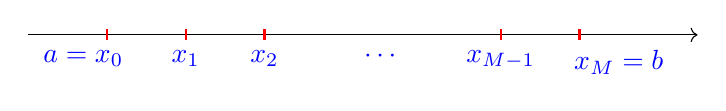
\begin{tikzpicture}
	\draw[->] (-1,0) -- (7.5,0);
		
	\foreach \i in {1,2}	
		\draw[red,thick] (\i,2pt)--(\i,-2pt) 
			node[text=blue,anchor=north]{$x_{\i}$};
	
	\draw[red,thick] (5,2pt)--(5,-2pt) 
		node[text=blue,anchor=north]{$x_{M-1}$};	
	\draw[red,thick] (0,2pt)--(0,-2pt)
		node[text=blue,anchor=north] at (-0.3,-2pt){$a=x_0$};
	\draw[red,thick] (6,2pt)--(6,-2pt) 
		node[text=blue,anchor=north] at (6.5,-2pt){$x_M=b$};
	\node[text=blue,anchor=north] at (3.5,-2pt) {$\cdots$};	
\end{tikzpicture}
		\caption{A partition on interval $[a,b]$}
		\label{tikz:1D_a_partition_on_interval_[a,b]}
	\end{figure}
	When talking about piecewise polynomials one has to fix a partitioning of 
	the domain $]a,b[$ first. Therefore we equip $\Omega=[a,b]$ with $M+1$ 
	nodes ($M\in \mathbb{N}$) forming the set (see Figure 
	\ref{tikz:1D_a_partition_on_interval_[a,b]})
	$$\mathcal{V}(\mathcal{M}):=\{a=x_0<x_1<...<x_{M-1}<x_M=b\}.$$
	The nodes define small intervals that constitute a mesh/grid
	$$\mathcal{M}:=\{]x_{j-1},x_j[:\; 1\leq j \leq M \}.$$		
	The intervals $[x_{j-1},x_j],\,j=1,...,M$ are the \emph{cells} of the 
	mesh $\mathcal{M}$, which is often identified with the set of its cells. 
	A special case is an equidistant mesh with uniformly spaced nodes:
	$$ x_j=a+jh,\quad h=\frac{b-a}{M}.$$		
	The local and global resolution of a mesh/grid is measured through two 
	quantities, the\[
	\begin{array}{lll@{}} % @{} suppresses the space between columns
	\textrm{(local) cell size}   &h_j:=|x_j-x_{j-1}|,\; j=1,...,M\\
	\textrm{(global) meshwidth}  &h_{\mathcal{M}}:=\displaystyle
													\max_j |x_j-x_{j-1}|.
	\end{array}\]

	\subsubsection{Meshes in 2D: Triangulations}
	\begin{figure}[!htbp]
		\centering
		\begin{minipage}{.5\textwidth}
			\centering
			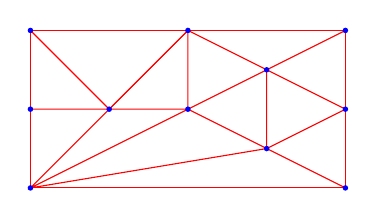
\begin{tikzpicture}
	\draw[red] (0,0) rectangle (4,2);
	\draw[red] (0,0)--(2,2)--(4,1)--(3,0.5)--(3,1.5)--
		(4,2)--(0,0)--(1,1)--(0,0)--(3,0.5)--(2,1)--(4,0);	
	\draw[red] (0,2)--(1,1)--(2,2)--(2,1)--(0,1);
	
	\foreach \p in {(0,0),(4,0),(3,.5),(0,1),(1,1),(2,1),
		(4,1),(3,1.5),(0,2),(2,2),(4,2)}	
		\fill[blue] \p circle (1pt);
\end{tikzpicture}
			\caption{Triangular mesh in 2D}
			\label{tikz:2D_triangular_mesh}
		\end{minipage}%
		\begin{minipage}{.5\textwidth}
			\centering
			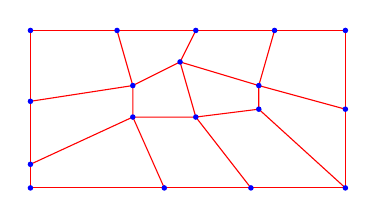
\begin{tikzpicture}
	\draw[red] (0,0) rectangle (4,2);
	\draw[red] (0,1.1)--(1.3,1.3)--(1.9,1.6)--(2.9,1.3)--(4,1);
	\draw[red] (0,.3) --(1.3,.9) --(2.1,.9) --(2.9,1);
	\draw[red] (1.1,2)--(1.3,1.3)--(1.3,.9)-- (1.7,0);
	\draw[red] (2.1,2)--(1.9,1.6)--(2.1,.9)-- (2.8,0);
	\draw[red] (3.1,2)--(2.9,1.3)--(2.9,1) -- (4,0);
		
	\foreach \p in {(0,0),(1.7,0),(2.8,0),(4,0),(4,1),(4,2),(3.1,2),(2.1,2),
		(1.1,2),(0,2),(0,1.1),(0,.3),(1.3,1.3),(1.3,.9),(1.9,1.6),(2.1,.9),
	 	(2.9,1.3),(2.9,1)}	
		\fill[blue] \p circle (1pt);
\end{tikzpicture}
			\caption{Quadrilateral mesh in 2D}
			\label{tikz:2D_quadrilateral_mesh}
		\end{minipage}
	\end{figure}

	\begin{figure}[!htbp]
		\centering
		\includegraphics[width=0.5\linewidth]{svg/2D_hybrid_mesh}
		\caption{A 2D \emph{hybrid} mesh comprising triangles,
		quadrilaterals, and curvilinear cells (at $\partial\Omega$)}
		\label{fig:2D_hybrid_mesh}
	\end{figure}	
	
	While in 1D splitting the interval into disjoint sub-intervals is about 
	the only meaningful option to define a partition, we have many more 
	possibilities in higher dimensions, for example, triangular mesh
	(Figure \ref{tikz:2D_triangular_mesh}), quadrilateral mesh
	(Figure \ref{tikz:2D_quadrilateral_mesh}), or hybrid mesh
	(Figure \ref{fig:2D_hybrid_mesh}), etc.
	Here we opt for triangulations, which are the most common meshes in two 
	dimensions. The definition of finite element triangulation and some 
	common parlance we use are given below:
	\begin{mdframed}[linecolor=blue,linewidth=.5pt,roundcorner=10pt]
	\begin{definition}[Triangulation]		
		A triangulation $\mathcal{M}$ of $\Omega$ satisfies 
		\begin{enumerate}[(i)]
			\item $\mathcal{M}=\{K_i\}_{i=1}^{M},\; M\in 
				\mathbb{R},\;K_i := $ open triangle
			\item disjoint interiors: $i\neq j \Rightarrow 
										K_i \cap K_j  = \varnothing$
			\item tiling/partition property: $ \displaystyle
				\bigcup_{i=1}^{M} \overline{K}_i=\overline{\Omega}$
			\item intersection $\overline{K}_i \cap \overline{K}_j,\,
			 	i\neq j$ is\\
					- either $\varnothing$,\\
					- or an edge of both triangles,\\
					- or a vertex of both triangles.
		\end{enumerate}
	\end{definition}
\end{mdframed}\label{def:triangulation}
%	\begin{mdfdef}[Triangulation]
	A triangulation $\mathcal{M}$ of $\Omega$ satisfies 
	\begin{enumerate}[(i)]
		\item $\mathcal{M}=\{K_i\}_{i=1}^{M},\; M\in 
			\mathbb{R},\;K_i := $ open triangle
		\item disjoint interiors: $i\neq j \Rightarrow 
									K_i \cap K_j  = \emptyset$
		\item tiling/partition property: $ \displaystyle
			\bigcup_{i=1}^{M} \overline{K}_i=\overline{\Omega}$
		\item intersection $\overline{K}_i \cap \overline{K}_j,\,
			i\neq j$ is\\
				- either $\emptyset$,\\
				- or an edge of both triangles,\\
				- or a vertex of both triangles.
	\end{enumerate}
\end{mdfdef}
	\begin{mdframed}[linecolor=orange,linewidth=.5pt,roundcorner=10pt]
	\begin{tabular}{llllll}
	 Common parlance: & vertices of triangles & = & nodes of mesh
			 & = & set $\mathcal{V}(\mathcal{M})$\\
	  				  & triangles of the mesh & = & cells or elements of mesh
			 & = & set $\mathcal{M}$
	\end{tabular}
\end{mdframed}
	
	\subsubsection{Space and Basis in 1D}\label{subsubsection.2.1.3}
	\begin{figure}[!htbp]
		\centering
		\begin{minipage}{.5\textwidth}
		\centering
		\input{input/tikz/1D_example_solution_Dir_homo}
		\caption{$\Uparrow$ a function $\in\mathcal{S}_{1,0}^{0}(\mathcal{M})$}
		\label{tikz:1D_example_solution_Dir_homo}
		\end{minipage}%
		\begin{minipage}{.5\textwidth}
		\centering
		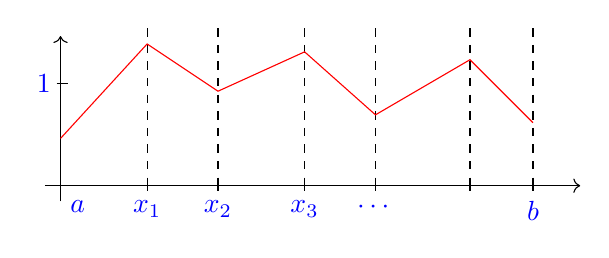
\begin{tikzpicture}
	\draw[->] (-.2,0) -- (6.6,0);
	\draw[->] (0,-.2) -- (0,1.9);	
	
	\draw (-.05,1.3)--(.1,1.3);	
	\foreach \x in {1.1,2,3.1,4,5.2,6}{
		\draw [dashed,thin] (\x,2cm)--(\x,2pt);
		\draw (\x,2pt)--(\x,-2pt);
	}
	\foreach \x/\i in {1.1/1,2,3.1/3}
		\node[text=blue,anchor=north] at (\x, -2pt) {$x_\i$};
	
	\node[text=blue,anchor=north] at (4, -2pt) {$\cdots$};
	\node[text=blue,anchor=north west] at (0, -2pt) {$a$};
	\node[text=blue,anchor=north] at (6, -2pt) {$b$};
	\node[text=blue,anchor=east] at (0,1.3) {1};
	
	\draw[red] 
	(0,.6)--(1.1,1.8)--(2,1.2)--(3.1,1.7)--(4,0.9)--(5.2,1.6)--(6,0.8);
\end{tikzpicture}
		\caption{$\Uparrow$ a function $\in \mathcal{S}_{1}^{0}(\mathcal{M})$}
		\label{tikz:1D_example_solution_Dir_inhomo}
		\end{minipage}
	\end{figure}
	For the 1D problem \hyperlink{P1}{P1}, we consider the simplest space of 
	continuous, $M$-piecewise polynomial functions in $H_0^1(]a,b[)$:
	\begin{equation}\label{def:1D S_10^0(M) space}
	U_h=\mathcal{S}_{1,0}^{0}(\mathcal{M}) := \left\{
	\begin{array}{l}
	v\in C^0{[a,b]}: v_{|[x_{i-1},x_i]}\ \textrm{linear},\\
	i=1,...,M,\ v(a)=v(b)=0
	\end{array}\right\},
	\end{equation}
	\[ N:=\mathrm{dim}\,\mathcal{S}_{1,0}^{0}(\mathcal{M})=M-1. \]	
	In above notation, the symbol $\mathcal{S}$ in 
	$\mathcal{\textcolor{red}{S}}_{1,0}^{0}$
	comes form the fact that the space 
	is comprised of scalar functions, the superscript $0$ in $ 
	\mathcal{S}_{1,0}^{\textcolor{red}{0}}$ is owing to $C^0[a,b]$
	 (continuous functions), the subscript $1$ 
	in  $\mathcal{S}_{\textcolor{red}{1},0}^{0}$ is due to the linearity 
	(locally 1st degree polynomials), 
	and the subscript $0$ in $\mathcal{S}_{1,\textcolor{red}{0}}^{0}$ is 
	because of being zero at the (homogeneous) boundary (see Figure 
	\ref{tikz:1D_example_solution_Dir_homo}). For a more general 
	two-point Dirichlet problem, we can define (see Figure 
	\ref{tikz:1D_example_solution_Dir_inhomo})
	
	\begin{equation}\label{def:1D S_1^0(M) space}
	\mathcal{S}_{1}^{0}(\mathcal{M}):=\left\{
		v\in C^0{[a,b]}: v_{|[x_{i-1},x_i]}\ \textrm{linear},\quad
			\forall i=1,...,M\right\}.
	\end{equation}
	
	\begin{figure}[!htbp]
		\centering		
		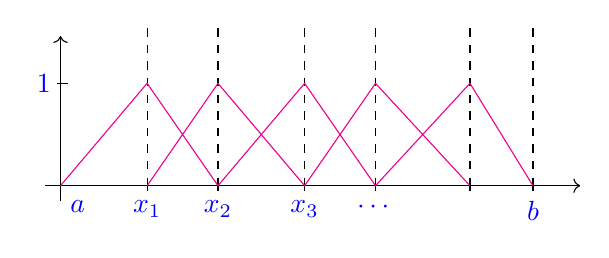
\begin{tikzpicture}
	\draw[->] (-.2,0) -- (6.6,0);
	\draw[->] (0,-.2) -- (0,1.9);	
	
	\draw (-.05,1.3)--(.1,1.3);	
	\foreach \x in {1.1,2,3.1,4,5.2,6}{
		\draw [dashed,thin] (\x,2cm)--(\x,2pt);
		\draw (\x,2pt)--(\x,-2pt);
	}
	\foreach \x/\i in {1.1/1,2,3.1/3}
		\node[text=blue,anchor=north] at (\x, -2pt) {$x_\i$};
	
	\node[text=blue,anchor=north] at (4, -2pt) {$\cdots$};
	\node[text=blue,anchor=north west] at (0, -2pt) {$a$};
	\node[text=blue,anchor=north] at (6, -2pt) {$b$};
	\node[text=blue,anchor=east] at (0,1.3) {1};
	
	\draw[magenta] (0,0)--(1.1,1.3)--(2,0)--(3.1,1.3)--(4,0)--(5.2,1.3)--(6,0) 
		(1.1,0)--(2,1.3)--(3.1,0)--(4,1.3)--(5.2,0);
\end{tikzpicture}
		\caption{1D tent functions in $\mathcal{S}_{1,0}^{0}(\mathcal{M})$}
		\label{tikz:1D_tent_functions}
	\end{figure}
	Our choice of the ordered basis 
	$\mathfrak{B}_h=\{b_h^1, ..., b_h^{M-1}\}$ of $U_h$ is	the 1D tent 
	functions (see Figure \ref{tikz:1D_tent_functions}):
	\begin{equation}\label{def:1D tent functions}
	b_h^j(x) := 
	\begin{cases}
		(x-x_{j-1})/h_j, 	  & \textrm{if}\ x_{j-1}\leq x\leq x_j,\\
		(x_{j+1}-x)/h_{j+1},  & \textrm{if}\ x_{j}\leq x\leq x_{j+1},\\
		0,					  & \textrm{elsewhere}.	
	\end{cases}	
	\end{equation}	
	\begin{equation}\label{pro:1D S_10^0(M) nodal (value) property}
	b_h^j(x_i) = \delta(x) := 
	\begin{cases}
		1, 	  & \textrm{if}\  i=j,\\
		0,    & \textrm{if}\  i\neq j.
	\end{cases}	
	\end{equation}
	In \eqref{eq:linear combi of u_h}, letting $x$ be the interior nodes of 
	the mesh ($x=x_j,\,j=1,...,M-1$) and 
	noting \eqref{pro:1D S_10^0(M) nodal (value) property} we have:
	\begin{equation}
	u_h\in \mathcal{S}_{1,0}^{0}(\mathcal{M}) \quad\Leftrightarrow\quad
		u_h=\sum_{i=1}^{M-1}u_h(x_i)b_h^i.
	\end{equation}
	
	\subsubsection{Space and Basis in 2D}
	\textbf{Linear Finite Element Space}\\[8pt]
	Now we examine the two-dimensional linear finite element space as well
	as the basis in 2D. Our first objective is to we 
	generalize the space $\mathcal{S}_{1}^{0}(\mathcal{M})$ 
	as defined in \eqref{def:1D S_1^0(M) space} to 2D. To do so we first 
	extend he concept of (affine) linear scalar-valued functions. Table 
	\ref{table:Affine_linear_functions} below exhibits the natural 
	correspondence of concepts in 1D and 2D. Then we define 
	$\mathcal{S}_{1}^{0}(\mathcal{M})$ over a 
	triangular mesh in 2D in the same fashion as we defined it in 1D over a 
	partition of an interval.
	\begin{table}[!htbp]
	\begin{mdframed}[linecolor=red,linewidth=.5pt,roundcorner=10pt]
		\centering
		\begin{tabular}{ccc}
	& $d=1$ & $d=2$\\
	\hline\\[0.5ex]
	Grid/mesh cells:  & intervals $]x_{i-1},x_i[,\; i=1,...,M$
	& triangles $K_i,\; i=1,...,M$\\[10pt]
	Linear functions: & $x\in\mathbb{R}\mapsto\alpha+\beta\cdot x,\;
	\alpha,\beta\in \mathbb{R}$ & 
	$\bx\in\mathbb{R}^2 \mapsto \alpha+\bm{\beta}\cdot\bx,\;
	\alpha\in\mathbb{R},\bm{\beta}\in\mathbb{R}^2$
\end{tabular}
		\caption{Affine linear functions in 1D and 2D}
		\label{table:Affine_linear_functions}
	\end{mdframed}
	\end{table}
	
	This suggests that we try a definition analogous to the 1D case 
	\eqref{def:1D S_1^0(M) space} (see Figure 
	\ref{fig:2D_piecewise_affine_linear_function_example}):
	\begin{equation}\label{def:2D S_1^0(M) space}
	U_h=\mathcal{S}_{1}^{0}(\mathcal{M}):=\left\{
	v\in C^0(\overline{\Omega}): \forall K\in\mathcal{M}:
	\begin{array}{l}
	v_{|K}(\bx)=\alpha_K+\bm{\beta}_K\cdot\bx,\\
	\alpha_K\in\mathbb{R}, \bm{\beta}_K\in\mathbb{R}^2, \bx\in K
	\end{array} \right\}\subset H^1(\Omega).
	\end{equation}
	The proof of the subset relationship above between 
	$\mathcal{S}_{1}^{0}(\mathcal{M})$ and $H^1(\Omega)$ involves
	the notion of \emph{weak derivatives} and thus will not be discussed 
	here but an intuitive theorem alongside a graph is given in
	the book \cite{Hiptmair} in 1.3.4.22. The theorem implies that a function 
	that is piecewise (with regard to a ``nice" partition of $\Omega$) smooth 
	and bounded belongs to $H^1(\Omega)$ if and only if it is continuous on 
	the entire domain $\Omega$, which accounts for the requirement of
	$C^0(\overline{\Omega})$ in the above definition.
	\begin{figure}[!htbp]
		\centering
		\includegraphics[width=0.7\linewidth]{
			svg/2D_piecewise_affine_linear_function_example}
		\caption{$\Uparrow$ a continuous piecewise affine linear function
			 $\in \mathcal{S}_{1}^{0}(\mathcal{M})$ on a triangular mesh
		 	 $\mathcal{M}$ }
		\label{fig:2D_piecewise_affine_linear_function_example}
	\end{figure}
	
	It can be seen that for 
	$u_h\in\mathcal{S}_{1}^{0}(\mathcal{M})$
	the gradient $\grad u_h$ can be computed on each 
	triangle as piecewise constant function, i.e.
	\begin{equation}\label{eq:2D gradient formula}
	\textrm{on}\ K\in\mathcal{M}:\ 
	\mathbf{grad}(\alpha_K+\bm{\beta}_K\cdot\bx)=\bm{\beta}_K.
	\end{equation}\\
	
	\noindent\textbf{Nodal Basis Functions}\\[8pt]		
	Our next goal is the generalization of ``tent functions", see
	\eqref{def:1D tent functions} and Figure \ref{tikz:1D_tent_functions}.
	In 1D, adding two more ``half-tent" functions (see the two 
	\textcolor{mid-green}{green} parts in Figure
	\ref{tikz:1D_tent_functions_in_S_1^0(M)}), cardinal basis functions
	belonging to the end points $x_0$ and $x_M$, we obtain a basis of
	$\mathcal{S}_{1}^{0}(\mathcal{M})$:
	\begin{equation}	
	\mathfrak{B}=\{b_h^0,...,b_h^M\},
	\end{equation}\vspace{-10pt}
	\begin{equation}
	b_h^j(x_i) = \delta(x) := 
	\begin{cases}
	1, 	  & \textrm{if}\  i=j,\\
	0,    & \textrm{if}\  i\neq j.
	\end{cases}	\label{pro:1D S_1^0(M) nodal (value) property}
	\end{equation}
	\begin{figure}[!htbp]
		\centering		
		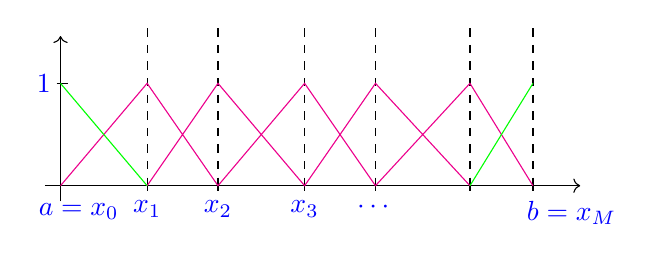
\begin{tikzpicture}
	\draw[->] (-.2,0) -- (6.6,0);
	\draw[->] (0,-.2) -- (0,1.9);	
	
	\draw (-.05,1.3)--(.1,1.3);	
	\foreach \x in {1.1,2,3.1,4,5.2,6}{
		\draw [dashed,thin] (\x,2cm)--(\x,2pt);
		\draw (\x,2pt)--(\x,-2pt);
	}
	\foreach \x/\i in {1.1/1,2,3.1/3}
		\node[text=blue,anchor=north] at (\x, -2pt) {$x_\i$};
	
	\node[text=blue,anchor=north] at (4, -2pt) {$\cdots$};
	\node[text=blue,anchor=north west] at (-.4, -3pt) {$a=x_0$};
	\node[text=blue,anchor=north west] at (5.8, -2pt) {$b=x_M$};
	\node[text=blue,anchor=east] at (0,1.3) {1};
	
	\draw[magenta] (0,0)--(1.1,1.3)--(2,0)--(3.1,1.3)--(4,0)--(5.2,1.3)--(6,0) 
		(1.1,0)--(2,1.3)--(3.1,0)--(4,1.3)--(5.2,0);
	\draw[green] (0,1.3)--(1.1,0) (5.2,0)--(6,1.3);
\end{tikzpicture}
		\caption{1D tent functions in $\mathcal{S}_{1}^{0}(\mathcal{M})$}
		\label{tikz:1D_tent_functions_in_S_1^0(M)}
	\end{figure}

	Actually, the ``nodal (value) property" condition 
	\eqref{pro:1D S_1^0(M) nodal (value) property}  already defines a tent 
	function in the space $\mathcal{S}_{1}^{0}(\mathcal{M})$. This approach
	is directly carried over to 2D: for any node 
	$\bx\in\mathcal{V}(\mathcal{M})$ we let it have height $1$, then together 
	with all its adjacent nodes they form a tent shape function (partial tent 
	shape on the boundary $\partial\Omega$), see Figure 
	\ref{fig:2D_nodal_basis_function_example} for an illustration.	
	\begin{figure}[!htbp]
		\centering
		\includegraphics[width=0.7\linewidth]{
			svg/2D_nodal_basis_function_example}
		\caption{A (global) piecewise linear nodal basis function on a
			triangular mesh $\mathcal{M}$  }
		\label{fig:2D_nodal_basis_function_example}
	\end{figure}
	
	From the above picture we can see that the basis function $b_h^i$ can be 
	viewed as the intersection of the $xOy$ plane and several slanted planes 
	of these local tetrahedrons on the adjacent triangles to vertex $x_i$. 
	Figure \ref{fig:2D_local_nodal_basis_function_example}
	shown on the next page is one of the six local nodal basis functions 
	that form the global piecewise linear nodal basis function
	in Figure \ref{fig:2D_nodal_basis_function_example}. Further more, from
	a triangle's perspective, if we look at each triangle on the mesh
	$\mathcal{M}$, each of the 3 vertices can serve as the \emph{pivot} so 
	that the slanted plane of this local tetrahedron constitutes one part of 
	the global tent function that is based on the \emph{pivot} (vertex).
	\begin{figure}[!htbp]
		\centering
		\includegraphics[width=0.7\linewidth]{
			svg/2D_local_nodal_basis_function_example}
		\caption{A local nodal basis function over a triangle with
			the pink node being the \emph{pivot}  }
		\label{fig:2D_local_nodal_basis_function_example}
	\end{figure}

	Thus, we can define the 2D counterpart of the 1D tent function basis  
	by ``nodal conditions"  in the following fashion:\\
	Writing 		
	$\mathcal{V}(\mathcal{M}) = \{\bx_1,...,\bx_N\}$, an ordering of the nodes
	is implied, the nodal basis $\mathfrak{B}_h=\{b_h^1,...,b_h^N\}$ of 
	$\mathcal{S}_{1}^{0}(\mathcal{M})$ satisfies the conditions
					
	\begin{minipage}{.5\textwidth}
	\begin{equation}\label{pro:2D S_1^0(M) nodal (value) property}	
	\begin{array}{l}
	b_h^j\in \mathcal{S}_{1}^{0}(\mathcal{M}),\\[8pt]
	b_h^j(\bx_i)=\begin{cases}
	1,\quad \textrm{if}\ \bx_i=\bx_j,\\
	0,\quad \textrm{if}\ \bx_i\in\mathcal{V}(\mathcal{M})\setminus \{\bx_j\},	
	\end{cases}\\[18pt]
	i,j=\{1,...,N\}.
	\end{array}
	\end{equation}
	\end{minipage}\hfil
	\begin{minipage}{.5\textwidth}
		\input{input/tikz/2D_piecewise_linear_nodal_basis_function}	
	\end{minipage}\\[8pt]
	
	Given the cardinal basis property of $\mathfrak{B}_h$ with respect to
	the node set $\mathcal{V}(\mathcal{M}) = \{\bx_1,...,\bx_N\}$ in 
	\eqref{pro:2D S_1^0(M) nodal (value) property}, the coefficients of the 
	nodal basis	expansion of a $u_h\in \mathcal{S}_{1}^{0}(\mathcal{M})$ 
	coincide with the nodal	values $u_h(\bx_i)$:
	\begin{equation}
	u_h\in \mathcal{S}_{1}^{0}(\mathcal{M}):\quad 
		u_h=\sum_{i=1}^{N}\mu_i b_h^i \quad\Leftrightarrow\quad 
		\mu_i = u_h(\bx_i) \quad \forall i=1,...,N.
	\end{equation}	
	
	\subsection{Computing Galerkin Matrices and R.H.S. Vectors}
	\subsubsection{In One-Dimension}\label{subsubsection.2.2.1}
	In Section \hyperref[subsubsection.2.1.3]{2.1.3} we have obtained
	the 1D tent basis functions	\[
	b_h^j(x) := 
	\begin{cases}
	(x-x_{j-1})/h_j, 	  & \textrm{if}\ x_{j-1}\leq x\leq x_j,\\
	(x_{j+1}-x)/h_{j+1},  & \textrm{if}\ x_{j}\leq x\leq x_{j+1},\\
	0,					  & \textrm{elsewhere}.	
	\end{cases} \]
	Then we can conclude that
	\begin{equation}\label{eq:1D Galerkin matrix terms vanish if |i-j|>=2}
	|i-j| \geq 2 \quad\Rightarrow\quad
	\frac{\rd b_h^j}{\rd x}(x)\frac{\rd b_h^i}{\rd x}(x)=0,\quad
	b_h^j(x) b_h^i(x)=0 \quad \forall x\in[a,b],
	\end{equation}	
	which follows from the fact that there is no overlap of supports
	of the two basis functions.
		
	Since by \eqref{eq:discrete ODE formulas}
	and  \eqref{eq:linear systems of equations formulas}
	\begin{equation}\label{eq:1D Galerkin a_ij general formula}
	(\bA)_{ij}=a(b_h^j,b_h^i)=\int_{a}^{b}\left(	
	p\frac{\rd b_h^j}{\rd x}\frac{\rd b_h^i}{\rd x}+q b_h^j b_h^i\right)\rd x,
	\end{equation}
	\eqref{eq:1D Galerkin matrix terms vanish if |i-j|>=2} suggests that the 
	Galerkin matrix for problem \hyperlink{P1}{P1} is \emph{tridiagonal} 
	(also \emph{symmetric} by \eqref{eq:1D Galerkin a_ij general formula}).
	\vspace{8pt}
	
	For simplicity, we first look at a simplest case where $p(x)=1,\ q(x)=0$.
	Noting that the gradients (derivatives) of the tent functions are 
	piecewise constant:
	\begin{equation}\label{eq:1D tent function derivatives}
	\frac{\rd b_h^j}{\rd x}=\begin{cases}
	h_{j},   \quad &\textrm{if}\ x_{j-1}\leq x\leq x_{j},\\
	-h_{j+1},\quad &\textrm{if}\ x_{j}\leq x\leq x_{j+1},\\
	0,	  	 \quad &\textrm{elsewhere},
	\end{cases}
	\end{equation}
	then it immediately follows that
	\begin{equation*}
	\int_{a}^{b}\frac{\rd b_h^j}{\rd x}(x)\frac{\rd b_h^i}{\rd x}(x)\,\rd x=
	\left\{
	\begin{array}{lll}
		0, &\textrm{if}\ |i-j|>2,  &\rightarrow \quad 
		\vcenter{\hbox{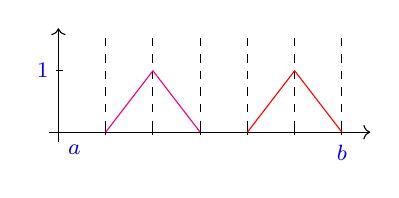
\begin{tikzpicture}[scale=0.6]
	\draw[->] (-.2,0) -- (6.6,0);
	\draw[->] (0,-.2) -- (0,2.2);	
	
	\draw (-.05,1.3)--(.1,1.3);	
	\foreach \i in {1,2,...,6}{
		\draw [dashed,thin] (\i,2cm)--(\i,2pt);
		\draw (\i,2pt)--(\i,-2pt);
	}
	
	\node[text=blue,anchor=north west] at (0, -2pt) {\footnotesize $a$};
	\node[text=blue,anchor=north] at (6, -2pt) {\footnotesize $b$};
	\node[text=blue,anchor=east] at (0,1.3) {\footnotesize 1};
		
	\draw[magenta] (1,0)--(2,1.3)--(3,0);
	\draw[red] (4,0)--(5,1.3)--(6,0);
\end{tikzpicture}}}\\
		
		-\dfrac{1}{h_{i+1}}, &\textrm{if}\ j=i+1, &\rightarrow \quad 
		\vcenter{\hbox{\input{input/tikz/1D_tents_j=i+1}}}\\
		
		-\dfrac{1}{h_{i}}, &\textrm{if}\ j=i-1, &\rightarrow \quad 
		\vcenter{\hbox{\input{input/tikz/1D_tents_j=i-1}}}\\
		
		\dfrac{1}{h_{i}}+\dfrac{1}{h_{i+1}},&\textrm{if}\ 1\leq i=j\leq M-1.
		&\rightarrow \quad \vcenter{\hbox{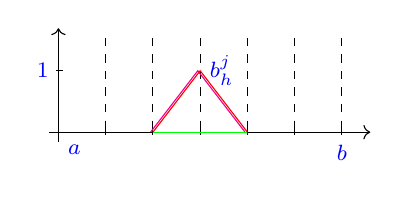
\begin{tikzpicture}[scale=0.6]
	\draw[->] (-.2,0) -- (6.6,0);
	\draw[->] (0,-.2) -- (0,2.2);	
	
	\draw (-.05,1.3)--(.1,1.3);	
	\foreach \i in {1,2,...,6}{
		\draw [dashed,thin] (\i,2cm)--(\i,2pt);
		\draw (\i,2pt)--(\i,-2pt);
	}
	
	\node[text=blue,anchor=north west] at (0, -2pt) {\footnotesize $a$};
	\node[text=blue,anchor=north] at (6, -2pt) {\footnotesize $b$};
	\node[text=blue,anchor=east] at (0,1.3) {\footnotesize 1};
		
	\draw[magenta] (1.95,0)--(2.95,1.3)--(3.95,0);
	\draw[red] (2,0)--(3,1.3)--(4,0)
		node[text=blue,anchor=west] at (3,1.3) {\footnotesize $b_h^j$};
	\draw[green] (2,0)--(4,0);
\end{tikzpicture}}}
	\end{array}\right.
	\end{equation*}	
	So we can obtain the following Galerkin matrix which is \emph{symmetric},
	\emph{positive definite}, and \emph{tridiagonal}:
	\begin{equation}\label{eq:1D simplest Galerkin matrix}
	\bA = \begin{bmatrix} 
	\frac{1}{h_1}+\frac{1}{h_2} & -\frac{1}{h_2} & 0 & & & &0\\
	-\frac{1}{h_2} & \frac{1}{h_2}+\frac{1}{h_3} &-\frac{1}{h_3} & & & &\\
	0 &\ddots &\ddots &\ddots & & & \\
	& & & & & & \\
	& & & & &\ddots &0 \\
	& & & &\ddots &\ddots &-\frac{1}{h_{M-1}} \\
	0 & & & &0 &-\frac{1}{h_{M-1}} &\frac{1}{h_{M-1}}+\frac{1}{h_{M}}
	\end{bmatrix}\in\mathbb{R}^{N,N},\quad N:=M-1.
	\end{equation}
	Specially, for an equidistant mesh $\mathcal{M}$ with uniform meshwidth
	$h>0$ the finite element linear system of equations 
	\eqref{eq:linear systems of equations} becomes
	\begin{equation}\label{eq:1D LSE on equidistant mesh}
	\frac{1}{h}\begin{bmatrix} 
	2 & -1 & 0 & & & &0\\
	-1 & 2 &-1 & & & &\\
	0 &\ddots &\ddots &\ddots & & & \\
	& & & & & & \\
	& & &\ddots &\ddots &\ddots &0 \\
	& & & &-1 &2 &-1 \\
	0 & & & &0 &-1 &2
	\end{bmatrix} \begin{bmatrix}
	\mu_1\\
		\\
	\vdots\\
		\\
	\mu_N
	\end{bmatrix}=h\begin{bmatrix}
	f(x_1)\\
		\\
	\vdots\\
		\\
	f(x_N)
	\end{bmatrix}.
	\end{equation}
	In fact, by combining the composite trapezoidal rule
	\begin{equation}\label{eq:composite trapezoidal rule}
	\int_{a}^{b} \psi(t) \, \rd t \approx 
		\sum_{j=1}^{M}\frac{1}{2}h_j(\psi(x_{j-1})+\psi(x_{j}))
	\end{equation}
	and the cardinal basis property 
	\eqref{pro:1D S_10^0(M) nodal (value) property} we have
	\begin{equation}\label{eq:1D RHS vector approx}
	\varphi_k:=(\vv{\bm{\varphi}})_k=\int_{a}^{b}f(x)b_h^k(x) \,\rd x
		\approx \frac{1}{2}(h_k+h_{k+1})f(x_k), \quad 1\leq k\leq N,
	\end{equation}
	which explains the right-hand side vector in 
	\eqref{eq:1D LSE on equidistant mesh}.\vspace{8pt}
	
	More generally, the Galerkin matrix and the right-hand side vector can be
	computed by the following formulas:
	\begin{equation}\label{eq:1D Galerkin matrix sub-diagonal terms formula}
	\begin{split}
	a(b_h^j,b_h^{j-1})=a(b_h^{j-1},b_h^j)
	&=\int_{x_{j-1}}^{x_j}\left[p\frac{\rd b_h^j}{\rd x}
		\frac{\rd b_h^{j-1}}{\rd x}+qb_h^j b_h^{j-1} \right]\rd x\\
	&=\int_{x_{j-1}}^{x_j}\left[-p(x)h_j^{-2}+
		q(x)b_h^j(x)b_h^{j-1}(x)\right]\rd x\\
	&=\int_{0}^{1}\left[-h_j^{-1}p(x_{j-1}+h_j\xi)+
		h_jq(x_{j-1}+h_j\xi) (1-\xi)\xi \right] \rd\xi,
	\end{split}
	\end{equation}	
	\begin{equation}\label{eq:1D Galerkin matrix diagonal terms formula}
	\begin{split}
	a(b_h^j,b_h^j)
	&=\int_{x_{j-1}}^{x_j}\left[p(\frac{\rd b_h^j}{\rd x})^2+ 		
		q(b_h^j)^2\right]\rd x +
	  \int_{x_j}^{x_{j+1}}\left[p(\frac{\rd b_h^j}{\rd x})^2+
	  	q(b_h^j)^2\right]\rd x\\
	&=\int_{x_{j-1}}^{x_j}\left[p(x)h_j^{-2}+q(x)(b_h^j(x))^2\right]\rd x+
	  \int_{x_j}^{x_{j+1}}\left[p(x)h_{j+1}^{-2}+q(x)(b_h^j(x))^2\right]\rd x\\
	&=\int_{0}^{1}\left[h_j^{-1}p(x_{j-1}+h_j\xi)+
		h_jq(x_{j-1}+h_j\xi)\xi^2\right]\rd\xi \; +\\
	  &\quad \int_{0}^{1}\left[h_{j+1}^{-1}p(x_j+h_{j+1}\xi)+
			h_{j+1}q(x_j+h_{j+1}\xi)(1-\xi)^2\right]\rd\xi,				
	\end{split}
	\end{equation}
	\begin{equation}\label{eq:1D RHS formula}
	\begin{split}
	(\vv{\bm{\varphi}})_j
	&=\int_{x_{j-1}}^{x_j}f(x)b_h^j(x) \, \rd x+
		\int_{x_j}^{x_{j+1}}f(x)b_h^j(x) \, \rd x\\
	&=h_j\int_{0}^{1} f(x_{j-1}+h_j\xi)\xi \, \rd\xi+
	  	h_{j+1}\int_{0}^{1} f(x_j+h_{j+1}\xi)(1-\xi) \, \rd\xi.
	\end{split}
	\end{equation}
	Here $j=2,...,N$ for
	\eqref{eq:1D Galerkin matrix sub-diagonal terms formula}, 
	and $j=1,...,N$ for 
	\eqref{eq:1D Galerkin matrix diagonal terms formula} and
	\eqref{eq:1D RHS formula}.\vspace{8pt}
	
	Next, we focus on the 2D computations of Galerkin matrix and RHS vector.
	Before the start of our computations we shall first look at the structures
	of Galerkin matrices.
		
	\subsubsection{Sparsity of Galerkin Matrix}
	We have learned from \hyperref[subsubsection.2.2.1]{previous}  
	sub-subsection that the Galerkin matrix is \emph{tridiagonal} under the 
	linear 	finite element Galerkin discretization in one dimension. In the
	2D counterpart, we can	also prove that it is always sparse, that is,
	most of its elements are zero.
	\begin{lemma}[Sparsity of Galerkin matrix {\cite[Lemma 2.4.4.2]{Hiptmair}}]
	\label{lma:Sparsity of Galerkin matrix}
	There is a constant $C>0$ depending only on the topology of $\Omega$,
	that is, the number of ``holes" in it, such that for any triangular mesh
	$\mathcal{M}$ of $\Omega$ ($N:=\sharp\mathcal{V}(\mathcal{M})=$ 
	number of vertices)
	\[\sharp\{(i,j)\in\{1,...,N\}^2:(\bA)_{ij}\neq0\}\leq 7\cdot N + C,\]
	where $\bA$ is any Galerkin matrix arising from a discretization of 
	a 2nd-order linear scalar elliptic variational problem with linear finite 
	elements.
	\end{lemma}
	\begin{proof}
	We rely on \href{https://en.wikipedia.org/wiki/Euler_characteristic}
	{Euler's formula} for triangulations.
	\[\sharp\mathcal{M}-\sharp\mathcal{E}(\mathcal{M})+
	\sharp\mathcal{V}(\mathcal{M})=\chi_\Omega,\quad \chi_\Omega=
	\textrm{Euler characteristic of } \Omega.\]
	Note that $\chi_\Omega$ is a topological invariant (alternating sum of 
	Betti numbers).\\
	By combinatorial considerations (traverse edges and count triangles):
	\[2\cdot\sharp\mathcal{E}_I(\mathcal{M})+\sharp\mathcal{E}_B(\mathcal{M})
		= 3\cdot\sharp\mathcal{M},\]
	where $\mathcal{E}_I(\mathcal{M}),\,\mathcal{E}_B(\mathcal{M})$ stands for
	the sets of interior and boundary edges of $\mathcal{M}$, respectively.\\
	Combining the above two equations yields
	\[\sharp\mathcal{E}_I(\mathcal{M})+2\cdot\sharp\mathcal{E}_B(\mathcal{M})
		= 3(\sharp\mathcal{V}(\mathcal{M})-\chi_\Omega).\]
	Then use
	\[N=\sharp\mathcal{V}(\mathcal{M}),\quad 
	\mathrm{nnz}(\bA)\leq N+2\cdot\sharp\mathcal{E}(\mathcal{M})
	\leq 7\cdot\sharp\mathcal{V}(\mathcal{M})-6\chi_\Omega,
	\]
	which implies the assertion for any triangulation.
	This completes the proof.
	\end{proof}
	
	\subsubsection{Computation of Galerkin Matrix}\label{subsubsection.2.2.3}
	Now we investigate an efficient algorithm for computing the non-zero 
	entries of the sparse finite element Galerkin matrix. For the sake of 
	simplicity, we shall, for the moment, drop the second term $\gamma(\bx)u$ 
	and let $\bm{\alpha}(\bx)$ be a $2\times2$ identity matrix in 
	\eqref{eq:PDE model} so that the bilinear form in
	\eqref{eq:discrete PDE formulas} becomes
	\[a(u_h,v_h):=\int_{\Omega}\grad u_h\cdot\grad v_h\,\dx,
		\quad u_h,v_h\in H^1(\Omega), \]
	thus leading the entries of the Galerkin matrix $\bA$ to
	\[(\bA)_{ij}=a(b_h^j,b_h^i)=
	\int_{\Omega}\grad b_h^j\cdot\grad b_h^i\, \dx.\]
	
	It is not hard to see that 
	\[\left\{\begin{array}{c}
	\textrm{Differing nodes } \bx_i,\bx_j\in\mathcal{V}(\mathcal{M})\\
	\textrm{that are not connected by an edge}
	\end{array}\quad\Leftrightarrow\quad
	\mathrm{Vol}(\mathrm{supp}(b_h^i)\cap\mathrm{supp}(b_h^j))=0\right\}
	\quad \Rightarrow \quad (\bA)_{ij}=0.
	\]\vspace{-20pt}	
	\begin{figure}[!htbp]
		\makebox[\textwidth][c]{
			\subfloat{\includegraphics[width=0.31\paperwidth]{svg/case1}}
			\subfloat{\includegraphics[width=0.31\paperwidth]{svg/case2}}
			\subfloat{\includegraphics[width=0.31\paperwidth]{svg/case3}}
		}
	\end{figure}

	Therefore, in order to compute $(\bA)_{ij}$ we only need to 
	deal with the situations where the two nodes $\bx_i,\bx_j\in
	\mathcal{V}(\mathcal{M})$ are either \emph{connected by an edge} of the 
	triangulation or \emph{coincide}.
	We shall first elaborate the former case.\vspace{8pt}
	
	When two nodes are connected by an edge, the edge can be either an 
	interior edge or a boundary edge. If it is an interior edge then it must
	be shared by two triangles whereas a boundary edge enjoys the full 
	ownership by a particular boundary triangle. For the first case we can
	think of $(\bA)_{ij}$ as the result of summing up the two triangles:
	
	\begin{minipage}{.5\textwidth}
		\begin{equation*}
		\begin{split}
		(\bA)_{ij}
		&=\int_{K_1}\grad b_{h|K_1}^j\cdot\grad b_{h|K_1}^i\, \dx\;+\\
		&\quad \int_{K_2}\grad b_{h|K_2}^j\cdot\grad b_{h|K_2}^i\, \dx		
		\end{split}
		\end{equation*}
	\end{minipage}%\hspace{-10pt}
	\begin{minipage}{.5\textwidth}
		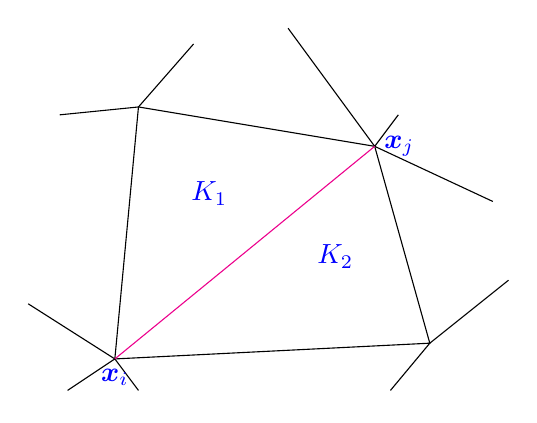
\begin{tikzpicture}
	\coordinate (A) at (0,0);
	\coordinate (B) at (4,0.2);
	\coordinate (C) at (3.3,2.7);
	\coordinate (D) at (0.3,3.2);
	
	\draw (A)--(B)--(C)--(D)--(A);	
	
	\draw (A)-- +(-.6,-.4) 		(A)-- +(.3,-.4)		(A)-- +(-1.1,.7);
	\draw (B)-- +(-.5,-.6) 		(B)-- +(1,.8);
	\draw (C)-- +(1.5,-.7) 		(C)-- +(.3,.4)	 	(C)-- +(-1.1,1.5);
	\draw (D)-- +(-1,-0.1) 		(D)-- +(.7,.8);
	
	\draw[magenta] (A)--(C);
	
	\node[text=blue] at (1.2,2.1) {$K_1$};
	\node[text=blue] at (2.8,1.3) {$K_2$};
	\node[text=blue,anchor=north] at (A) {$\bx_i$};
	\node[text=blue,anchor=west] at (C) {$\bx_j$};	
\end{tikzpicture}
	
	\end{minipage}\\[8pt]	
	While the boundary edge case can be understood as
	\[(\bA)_{ij}
		=\int_{K_\mathrm{B}}\grad b_{h|K_\mathrm{B}}^j
			\cdot\grad b_{h|K_\mathrm{B}}^i\, \dx,\]
	where $K_\mathrm{B}$ is a triangle on the boundary.
	
	In any cases, we can view them as 
	\emph{summing \textbf{cell contributions}}, 
	that is, if an edge is shared by two cells (triangles) then add them up, 
	if it is only owned by a single cell (triangle) then add this single one. 
	This idea is termed as \emph{\textbf{assembly}}, which is the \emph{key}
	to implementing the finite element method.\\
	
	\noindent\textbf{Local Computations}\\[8pt]
	Motivated by the formulas above we now fix our attention on a single 
	triangle $K\in\mathcal{M}$, restrict the bilinear form to it, and examine 
	the	cell contribution
	\begin{equation}
	a_K(b_h^j,b_h^i)=\int_K\grad b_{h|K}^j\cdot\grad b_{h|K}^i\, \dx,\quad
		\bx_i,\bx_j \ \textrm{nodes}\in\textrm{vertices of }K.
	\end{equation}
	Thus it is desirable if we could find out the analytic formulas for the 
	restrictions $b_{h|K}^i$. Let $\ba_K^1,\ba_K^2,\ba_K^3$ be the vertices of 
	the	triangle $K$ with coordinates $
	\ba_K^1=\begin{bmatrix}a^1_1\\a^1_2\end{bmatrix},\ 
	\ba_K^2=\begin{bmatrix}a^2_1\\a^2_2\end{bmatrix},\ \textrm{and }
	\ba_K^3=\begin{bmatrix}a^3_1\\a^3_2\end{bmatrix}$, we write
	\begin{equation}\label{def:baraycentric coordinate function}
	\lambda_i:=b_{h|K}^j \quad \textrm{with} \quad \ba_K^i=\bx_j. \quad 
	\left[\begin{array}{l}
	i \leftrightarrow \textrm{\emph{local} vertex number}\\
	j \leftrightarrow \textrm{\emph{global} node number}	
	\end{array}\right]
	\end{equation}
	Obviously, we have 3 such functions $\lambda_1,\lambda_2,\lambda_3$
	on any triangle $K\in\mathcal{M}$ with $x_j$ being the 3 vertices 
	of the triangle respectively, for example, the \textcolor{mid-green}{green} 
	surface given in Figure \ref{tikz:2D_barycentric_coordinate_function} 
	represents the graph of $\lambda_2$.
	\begin{figure}[!htbp]
		\centering
		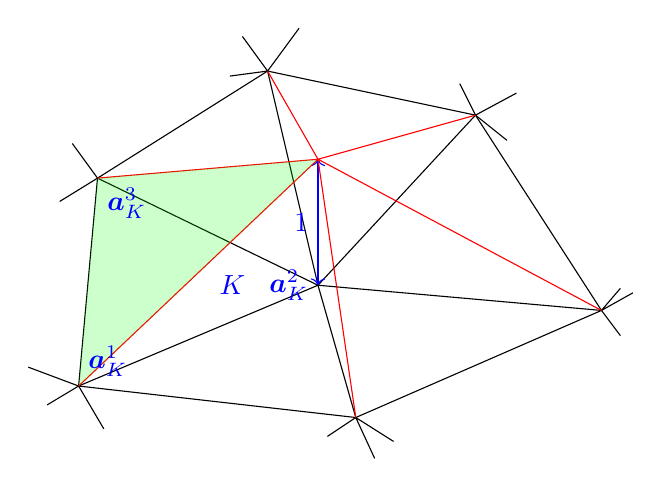
\begin{tikzpicture}[scale=.8]
%            (D)
%		    /   \
%     (E)  /	 \ (C)
%		  |	      |
%     (F) |	      | (B)
%  	       \     /  
%           \   / 
%            (A)

	\coordinate (O) at (0,0); \coordinate (T) at (0,2);
	\coordinate (A) at (0.6,-2.1);
	\coordinate (B) at (4.5,-0.4);
	\coordinate (C) at (2.5,2.7);
	\coordinate (D) at (-0.8,3.4);
	\coordinate (E) at (-3.5,1.7);
	\coordinate (F) at (-3.8,-1.6);
	\draw (A)--(B)--(C)--(D)--(E)--(F)--(A);
	\draw (O)--(A) (O)--(B) (O)--(C) (O)--(D) (O)--(E) (O)--(F);	
	
	\draw (A)-- +(-.45,-.3) 	(A)-- +(.3,-.65)	 (A)-- +(.6,-.38);
	\draw (B)-- +(.3,-.4) 		(B)-- +(.3,.35)	 	 (B)-- +(.5,.28);
	\draw (C)-- +(-.25,.5) 		(C)-- +(.65,.35)	 (C)-- +(.5,-.4);
	\draw (D)-- +(-.6,-.08) 	(D)-- +(-.4,.55)	 (D)-- +(.5,.68);
	\draw (E)-- +(-.6,-.37) 	(E)-- +(-.4,.55);
	\draw (F)-- +(-.8,.3) 		(F)-- +(-.5,-.3)	 (F)-- +(.4,-.68);
	
	\draw[blue,<->] (O)--(T);
	\draw[red] (T)--(A) (T)--(B) (T)--(C) (T)--(D) (T)--(E) (T)--(F);
	\node[text=blue,anchor=east] at (0,1) {$1$}; 
	
	\fill[green, opacity=0.2] (T)--(E)--(F)--(T);
	\node[text=blue,anchor=east] at (-1,0) {$K$};
	\node[text=blue,anchor=south west] at (F) {$\ba_{K}^{1}$};
	\node[text=blue,anchor=east] at (O) {$\ba_{K}^{2}$};
	\node[text=blue,anchor=north west] at (E) {$\ba_{K}^{3}$};
	
\end{tikzpicture}

		\caption{$\Uparrow$ a barycentric coordinate function 
			$\textcolor{mid-green}{\lambda_2}$}
		\label{tikz:2D_barycentric_coordinate_function}
	\end{figure}
	
	The functions $\lambda_1,\lambda_2,\lambda_3$ on the triangle $K$ are 
	also known as barycentric coordinate functions, which owe their name
	to the fact that they can be regarded as ``coordinates of a point with 
	respect to the vertices of a triangle" in the sense that
	\begin{equation}\label{eq:2D barycentric origin}
	 	\bx=\lambda_1(\bx)\ba_K^1+\lambda_2(\bx)\ba_K^2+\lambda_3(\bx)\ba_K^3.
	\end{equation}
	For instance, say, $
	\bx=\begin{bmatrix}x_1\\x_2\end{bmatrix},\ 
	\ba_K^1=\begin{bmatrix}0\\0\end{bmatrix},\ 
	\ba_K^2=\begin{bmatrix}1\\0\end{bmatrix},\ \textrm{and }
	\ba_K^3=\begin{bmatrix}0\\1\end{bmatrix}$, then
	$ \lambda_1(\bx)=1-x_1-x_2,\ 
	  \lambda_2(\bx)=x_1,\ 
	  \lambda_3(\bx)=x_2.$
	According to \eqref{eq:2D barycentric origin}, the following equation 
	holds true:	
	\[\bx=(1-x_1-x_2)\begin{bmatrix}0\\0\end{bmatrix}+
	 x_1\begin{bmatrix}1\\0\end{bmatrix}+
	 x_2\begin{bmatrix}0\\1\end{bmatrix}. \]
	
	In addition, as the attribute ``barycentric" indicates, the barycentric 
	coordinate functions $\lambda_1,\lambda_2,\lambda_3$ satisfy
	\[ \lambda_1+\lambda_2+\lambda_3=1. \]
	
	For the sake of comparison, we plot the graphs of the
	functions $\lambda_1,\lambda_2,\lambda_3$ in alignment:\vspace{-8pt}
	\begin{figure}[!htbp]
	\makebox[\textwidth][c]{
		\subfloat{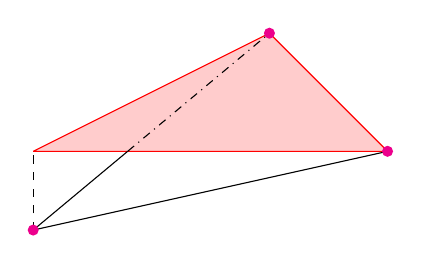
\begin{tikzpicture}	
	\coordinate (A) at (0,0); % pivot
	\coordinate (B) at (3,2.5); 
	\coordinate (C) at (4.5,1);
		
	\coordinate (T) at (0,1);
	
	\draw (A)--(C);
	\draw[dashed] (A)--(T);
	\fill[red!20] (T)--(B)--(C)--(T);
	\draw[red]	(T)--(B)--(C)--(T);
	
	\draw (A)--(1.2,1);
	\draw [dash dot] (1.2,1)--(B);
	
	\foreach \p in {(A),(B),(C)}
		\fill[magenta] \p circle (2pt);
\end{tikzpicture}}
		\hspace{5pt}
		\subfloat{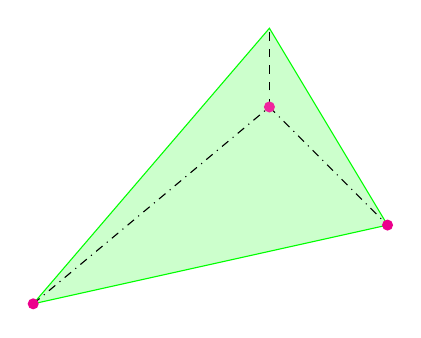
\begin{tikzpicture}	
	\coordinate (A) at (0,0);
	\coordinate (B) at (3,2.5); % pivot
	\coordinate (C) at (4.5,1);

	\coordinate (T) at (3,3.5);	
	
	\fill[green!20] (A)--(T)--(C)--(A);
	\draw[green] (A)--(T)--(C)--(A);
	\draw[dash dot] (A)--(B)--(C);
	\draw[dashed] (B)--(T);
	
	\foreach \p in {(A),(C)}	
		\fill[magenta] \p circle (2pt);
	\fill[magenta!85] (B) circle (2pt);
\end{tikzpicture}}
		\hspace{5pt}
		\subfloat{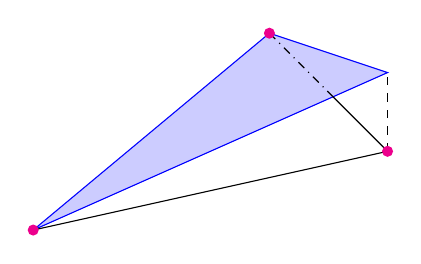
\begin{tikzpicture}	
	\coordinate (A) at (0,0);
	\coordinate (B) at (3,2.5);
	\coordinate (C) at (4.5,1); % pivot	

	\coordinate (T) at (4.5,2);
	
	\draw[dashed] (C)--(T);
	\fill[blue!20] (A)--(B)--(T)--(A);
	\draw[blue] (A)--(B)--(T)--(A);
	
	\draw (A)--(C)--(3.8,1.7);
	\draw[dash dot] (B)--(3.8,1.7);
	
	\foreach \p in {(A),(B),(C)}	
		\fill[magenta] \p circle (2pt);
\end{tikzpicture}}
	}
	\end{figure}
	
	Since the barycentric coordinate functions 
	$\lambda_1,\lambda_2,\lambda_3$ are affine linear functions (visually, 
	their graphs are planes) and for any fixed triangle $K\in\mathcal{M}$
 	they meet the cardinal basis property
	\eqref{pro:2D S_1^0(M) nodal (value) property}, we can write
	\begin{equation}
		\lambda_i(\bx)=\alpha_i+\bm{\beta}^i\cdot\bx,
	\end{equation}
	and on a triangle $K$ with coordinates $
	\ba_K^1=\begin{bmatrix}a^1_1\\a^1_2\end{bmatrix},\ 
	\ba_K^2=\begin{bmatrix}a^2_1\\a^2_2\end{bmatrix},\ \textrm{and }
	\ba_K^3=\begin{bmatrix}a^3_1\\a^3_2\end{bmatrix}$,
	they satisfy
	\begin{equation}\label{eq:barycentric LSF}
		\begin{bmatrix}
			1 &a^1_1 &a^1_2\\
			1 &a^2_1 &a^2_2\\
			1 &a^3_1 &a^3_2
		\end{bmatrix}
		\begin{bmatrix}
			\alpha_1  &\alpha_2  &\alpha_3\\
			\beta^1_1 &\beta^2_1 &\beta^3_1\\
			\beta^1_2 &\beta^2_2 &\beta^3_2
		\end{bmatrix}=
		\begin{bmatrix}
			1 &0 &0\\
			0 &1 &0\\
			0 &0 &1
		\end{bmatrix}.	
	\end{equation}
	
	Now we define the \emph{element (stiffness) matrix}
	\begin{equation}\label{def:2D element (stiffness) matrix}
		\bA_K:=\left[\int_K\grad\lambda_i\cdot
			\grad\lambda_j\,\dx\right]_{i,j=1}^3\in\mathbb{R}^{3,3}.
	\end{equation}	
	
	By \eqref{eq:2D gradient formula}, we have
	\begin{equation}
		\grad \lambda_i = \bm{\beta}^i,
	\end{equation}
	which, together with \eqref{eq:barycentric LSF}, suggests an efficient 
	way to compute the element (stiffness) matrix 
	\eqref{def:2D element (stiffness) matrix}:
	\begin{equation}\label{eq:2D element (stiffness) matrix formula}
		\bA_K=|K|
		\begin{bmatrix}
			\beta^1_1 &\beta^2_1 &\beta^3_1\\
			\beta^1_2 &\beta^2_2 &\beta^3_2			
		\end{bmatrix}^\top
		\begin{bmatrix}
			\beta^1_1 &\beta^2_1 &\beta^3_1\\
			\beta^1_2 &\beta^2_2 &\beta^3_2			
		\end{bmatrix}\in\mathbb{R}^{3,3},
	\end{equation}
	where $
	\begin{bmatrix}
		\beta^1_1 &\beta^2_1 &\beta^3_1\\
		\beta^1_2 &\beta^2_2 &\beta^3_2			
	\end{bmatrix}$
	can be computed by
	\begin{equation}\label{eq:2D element (stiffness) matrix component}
		\begin{bmatrix}
			\beta^1_1 &\beta^2_1 &\beta^3_1\\
			\beta^1_2 &\beta^2_2 &\beta^3_2			
		\end{bmatrix}=
		\left(\begin{bmatrix}
			1 &a^1_1 &a^1_2\\
			1 &a^2_1 &a^2_2\\
			1 &a^3_1 &a^3_2
		\end{bmatrix}^{-1}\right)_{(2:3,:)}.
	\end{equation}
	Here the notation $(2:3,:)$ in the above equation 
	\eqref{eq:2D element (stiffness) matrix component} is adopted from
	MATLAB, meaning the submatrix taken from the 2nd row to the 3rd row.
	
	\begin{remark}
	$\bA_K$ does not depend on the ``size" of triangle $K$.
	This is	followed by the reasoning below:
	\begin{itemize}
		\item Apparently, translation and rotation of $K$ does not
			change $\bA_K$.
		\item Scaling of $K$ by a factor $\rho>0$ has the effect that
		\begin{itemize}
			\item the area $|K|$ is scaled by $\rho^2$,
			\item the gradients $\grad \lambda_i$ are scaled by $\rho^{-1}$
				(imagine the graphs of $\lambda_i$: when the triangle shrinks 
				with $\rho<1$, they become steeper, otherwise flatter.)
		\end{itemize}
		Combining the two effects above offset the scaling of the
		triangle $K$, thus rendering $\bA_K$ invariant.			
	\end{itemize}
	\end{remark}\vspace{8pt}
	
	\noindent\textbf{Assembly of Full Galerkin Matrix}\\[8pt]	
	Now we consider the computation of the full Galerkin matrix. This time 
	our idea \emph{assembly} mentioned before comes in handy. The computation
	of $\bA_{ij}$ for $i\neq j$ starts from summing cell contributions
	\[(\bA)_{ij}=
	\int_{K_1}\grad b_{h|K_1}^j\cdot\grad b_{h|K_1}^i\, \dx +
	\int_{K_2}\grad b_{h|K_2}^j\cdot\grad b_{h|K_2}^i\, \dx, \]
	which can be visualized as follows:	
	\begin{figure}[!htbp]
		\centering
		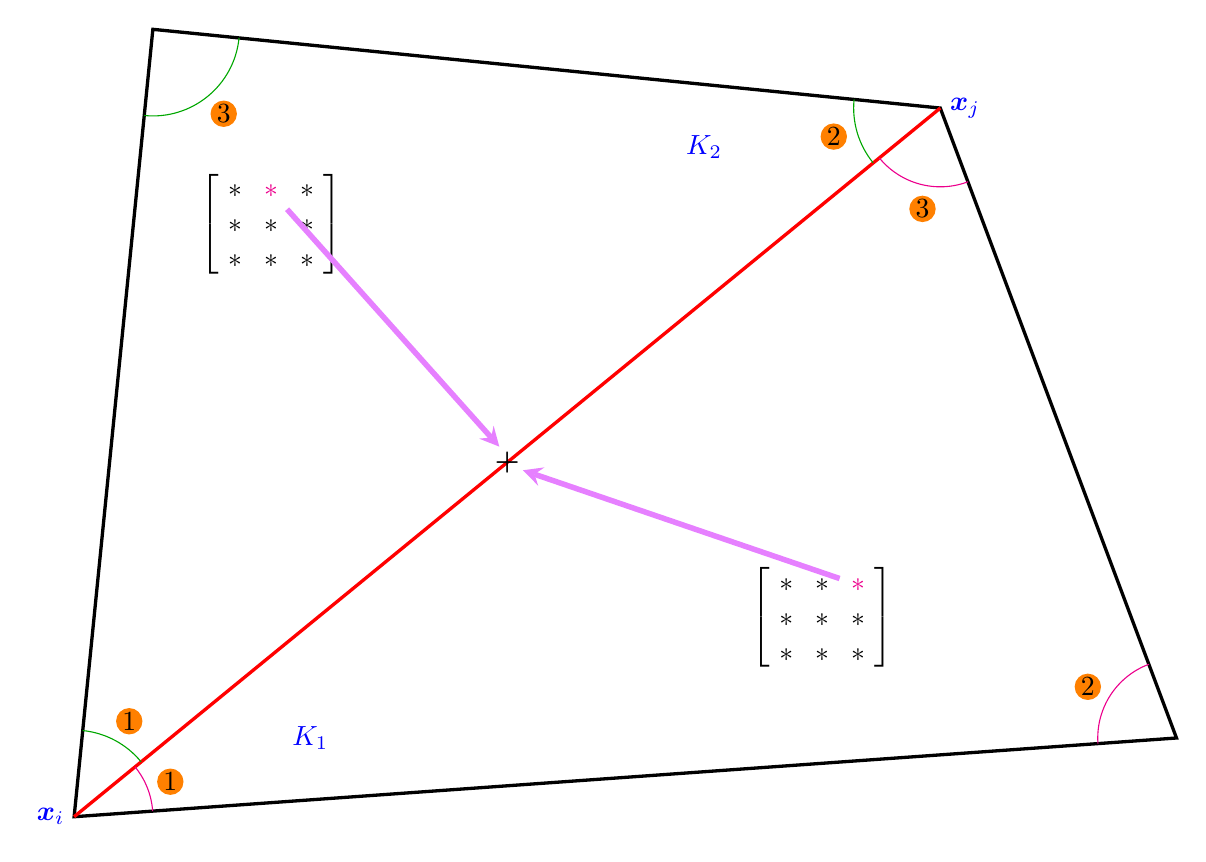
\begin{tikzpicture}	[
%	every left delimiter/.style={xshift=.75em},
%	every right delimiter/.style={xshift=-.75em},
	>=stealth
	]
	
	\coordinate (A) at (0,0);
	\coordinate (B) at (14,1);
	\coordinate (C) at (11,9);
	\coordinate (D) at (1,10);
	\coordinate (E) at (5.5,4.5); % midpoint of AC
	
	\draw[very thick] (A)--(B)--(C)--(D)--cycle;
	\draw[red, very thick] (A)--(C);
	
	% or use `angle` library
	\tkzMarkAngle[size=1cm,color=magenta,mark=none](B,A,C)
	\tkzMarkAngle[size=1cm,color=magenta,mark=none](C,B,A)
	\tkzMarkAngle[size=1cm,color=magenta,mark=    ](A,C,B)
	\tkzMarkAngle[size=1.1cm,color=mid-green,mark=none](D,C,A)
	\tkzMarkAngle[size=1.1cm,color=mid-green,mark=none](A,D,C)
	\tkzMarkAngle[size=1.1cm,color=mid-green,mark=none](C,A,D)
	
	
	\matrix [matrix of math nodes,
		left delimiter={[},
		right delimiter={]},
		inner sep=-2pt, 
%		inner ysep=-2pt,
		nodes={inner sep=.4em},
		row 1 column 2/.style=magenta,
		](M1) at (2.5,7.5) {
		* &* &*\\
		* &* &*\\
		* &* &*\\ % NOTE that \\ is necessary even for the last row
	};
%	\node (M1) at (2.5,7.5) {
%		$\begin{bmatrix}
%			* &\textcolor{magenta}{*} &*\\
%			* &* &*\\
%			* &* &*
%		\end{bmatrix}$	
%	};
	\matrix [matrix of math nodes,	
		left delimiter={[},
		right delimiter={]},
		inner sep=-2pt, 
		inner ysep=-2pt,
		nodes={inner sep=.4em},
		row 1 column 3/.style=magenta,
		](M2) at (9.5,2.5) {
		* &* &*\\
		* &* &*\\
		* &* &*\\
	};

	\node at (E) {$\boldsymbol{+}$};
	\draw[<-,line width=2pt,blue!20!magenta!50]
		(E)+(-.1,.2) -- (M1-1-2);
	\draw[<-,line width=2pt,blue!20!magenta!50]
		(E)+(.2,-.1) -- (M2-1-3);
		
	\path
		(A)++(60:1.4cm) node[fill=orange,circle,inner sep=.5pt] {$1$}
	 	(A)++(20:1.3cm) node[fill=orange,circle,inner sep=.5pt] {$1$}
	 	(B)++(150:1.3cm) node[fill=orange,circle,inner sep=.5pt] {$2$}
	 	(C)++(-100:1.3cm) node[fill=orange,circle,inner sep=.5pt] {$3$}
	 	(C)++(195:1.4cm) node[fill=orange,circle,inner sep=.5pt] {$2$}
	 	(D)++(-50:1.4cm) node[fill=orange,circle,inner sep=.5pt] {$3$};
	
	
	\node[text=blue] at (3,1) {$K_1$};
	\node[text=blue] at (8,8.5) {$K_2$};
	\node[text=blue,anchor=east] at (A) {$\bx_i$};
	\node[text=blue,anchor=west]  at (C) {$\bx_j$};
\end{tikzpicture}

		\caption{$\bA_{ij}$ by summing entries of two element matrices}
		\label{tikz:2D_assemble_two_element_matrices}
	\end{figure}

	In the above diagram, \orangecircled{1}, \orangecircled{2}, and
	\orangecircled{3} represent the local vertex numbers; the magenta
	entries $\textcolor{magenta}{*}$ in the element matrices of $K_1$ and
	$K_2$ are the items that have contributions to $\bA_{ij}$ 
	(expressed by the edge, note the directivity, however, that 
	$\bA_{ij}$ is contributed by \orangecircled{1}\orangecircled{3} 
	from $K_1$ alongside \orangecircled{1}\orangecircled{2} from $K_2$
	whereas $\bA_{ji}$ is contributed by 
	\orangecircled{3}\orangecircled{1} from $K_1$ and
 	\orangecircled{2}\orangecircled{1} from $K_2$. But in this thesis, the
 	bilinear form $a(\cdot,\cdot)$ we use will all be symmetric thus the 
 	Galerkin matrix $\bA$ and the element matrix $\bA_K$ from 
 	\eqref{def:2D element (stiffness) matrix} will also be 
 	symmetric,\footnote{
 	Indeed, whether the Galerkin matrix is symmetric is determined by a couple 
 	of factors: if the bilinear form is symmetric, how ever the boundary 
 	conditions are imposed, if we choose to use the same kinds of 
 	trial and test functions. By the Galerkin method we make it to the 1st and 
 	the 3rd ones, while the second one in real-world problems will 
 	usually render the final Galerkin matrix non-symmetric. But prior to 
 	processing the boundary conditions, the Galerkin matrix can be symmetric.
 	This can be verified from numerical example \hyperref[code:example1]{1}
 	in Section \hyperref[subsection.5.1]{5.1}.
 	}
 	so quantitatively speaking the directivity doesn't 
 	really matter. Otherwise we should make sure the relations are right).
	
	As for the assembly of the diagonal entry $\bA_{ii}$ of 
	the Galerkin matrix $\bA$, it can be obtained by summing 
	corresponding diagonal entries of element matrices belonging to triangles 
	adjacent to node $x_i$ (see Figure 
	\ref{tikz:2D_assemble_diagonal_element_matrices}).
	\begin{figure}[!htbp]
		\centering
		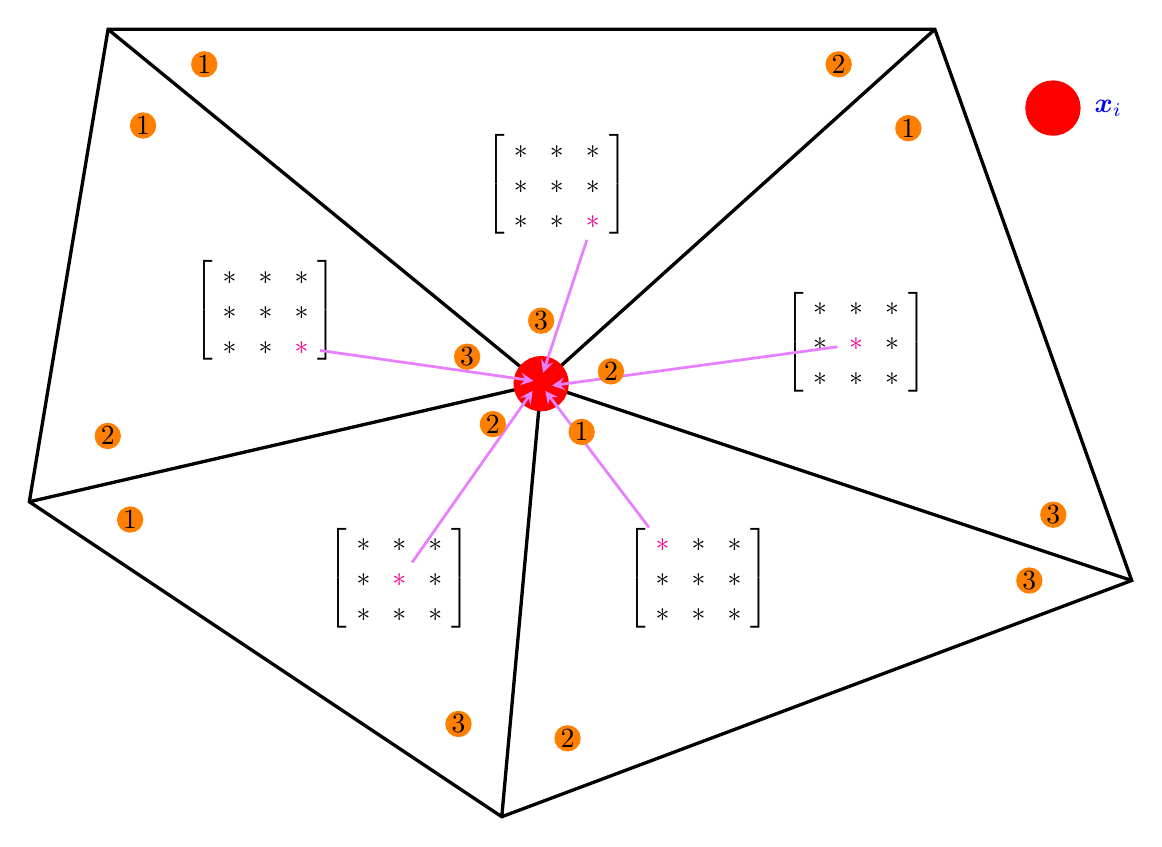
\begin{tikzpicture}	[>=stealth]
	
	\coordinate (A) at (6,0);
	\coordinate (B) at (14,3);
	\coordinate (C) at (11.5,10);
	\coordinate (D) at (1,10);
	\coordinate (E) at (0,4);
	
	\coordinate (F) at (6.5,5.5); % the center, focus
	\coordinate (X) at (13,9);    % commentary node
	
	\coordinate (O1) at (8.5,3);
	\coordinate (O2) at (10.5,6);
	\coordinate (O3) at (6.7,8);
	\coordinate (O4) at (3,6.4);
	\coordinate (O5) at (4.7,3);
	
	\draw[very thick] (A)--(B)--(C)--(D)--(E)--cycle
		(F)--(A) (F)--(B) (F)--(C) (F)--(D) (F)--(E);
	\fill[red] (F) circle (10pt)  (X) circle (10pt);
	
	\path (X)++(0:20pt) node[text=blue]{$\bx_i$};
	
	\matrix [matrix of math nodes,
		left delimiter={[},
		right delimiter={]},
		inner sep=-2pt,
		nodes={inner sep=.4em},
		row 1 column 1/.style=magenta,
		](M1) at (O1) {
		* &* &*\\
		* &* &*\\
		* &* &*\\
	};
	\matrix [matrix of math nodes,
	left delimiter={[},
	right delimiter={]},
	inner sep=-2pt,
	nodes={inner sep=.4em},
	row 2 column 2/.style=magenta,
	](M2) at (O2) {
		* &* &*\\
		* &* &*\\
		* &* &*\\
	};
	\matrix [matrix of math nodes,
	left delimiter={[},
	right delimiter={]},
	inner sep=-2pt,
	nodes={inner sep=.4em},
	row 3 column 3/.style=magenta,
	](M3) at (O3) {
		* &* &*\\
		* &* &*\\
		* &* &*\\
	};
	\matrix [matrix of math nodes,
	left delimiter={[},
	right delimiter={]},
	inner sep=-2pt,
	nodes={inner sep=.4em},
	row 3 column 3/.style=magenta,
	](M4) at (O4) {
		* &* &*\\
		* &* &*\\
		* &* &*\\
	};
	\matrix [matrix of math nodes,
	left delimiter={[},
	right delimiter={]},
	inner sep=-2pt,
	nodes={inner sep=.4em},
	row 2 column 2/.style=magenta,
	](M5) at (O5) {
		* &* &*\\
		* &* &*\\
		* &* &*\\
	};

	\draw[<-,line width=1pt,blue!20!magenta!50]
		(F)+(-60:3pt) -- (M1-1-1);
	\draw[<-,line width=1pt,blue!20!magenta!50]	
		(F)+(-10:4pt) -- (M2-2-2);	
	\draw[<-,line width=1pt,blue!20!magenta!50]	
		(F)+(80:4pt) -- (M3-3-3);
	\draw[<-,line width=1pt,blue!20!magenta!50]	
		(F)+(160:3pt) -- (M4-3-3);
	\draw[<-,line width=1pt,blue!20!magenta!50]	
		(F)+(-140:4pt) -- (M5-2-2);	
		
	\path
		(F)++(-50:.8cm) node[fill=orange,circle,inner sep=.5pt] {$1$}
		(F)++(10:.9cm) node[fill=orange,circle,inner sep=.5pt] {$2$}
		(F)++(90:.8cm) node[fill=orange,circle,inner sep=.5pt] {$3$}
		(F)++(160:1cm) node[fill=orange,circle,inner sep=.5pt] {$3$}
		(F)++(-140:.8cm) node[fill=orange,circle,inner sep=.5pt] {$2$}
		
		(A)++(115:1.3cm) node[fill=orange,circle,inner sep=.5pt] {$3$}
		(A)++(50:1.3cm) node[fill=orange,circle,inner sep=.5pt] {$2$}
	 	(B)++(180:1.3cm) node[fill=orange,circle,inner sep=.5pt] {$3$}
	 	(B)++(140:1.3cm) node[fill=orange,circle,inner sep=.5pt] {$3$}
	 	(C)++(-105:1.3cm) node[fill=orange,circle,inner sep=.5pt] {$1$}
	 	(C)++(-160:1.3cm) node[fill=orange,circle,inner sep=.5pt] {$2$}
	 	(D)++(-20:1.3cm) node[fill=orange,circle,inner sep=.5pt] {$1$}
	 	(D)++(-70:1.3cm) node[fill=orange,circle,inner sep=.5pt] {$1$}
	 	(E)++(40:1.3cm) node[fill=orange,circle,inner sep=.5pt] {$2$}
	 	(E)++(-10:1.3cm) node[fill=orange,circle,inner sep=.5pt] {$1$};
	 		 
	
\end{tikzpicture}

		\caption{$\bA_{ii}$ by summing diagonal entries of element
			 matrices of adjacent triangles}
		\label{tikz:2D_assemble_diagonal_element_matrices}
	\end{figure}
	
	Therefore, combining the two situations above we can develop a 
	vertex-oriented assembly algorithm as follows:
	\begin{algorithm}[!htbp]
		\caption{Vertex-centered assembly of Galerkin matrix for
			 linear finite elements}
		\label{alg:assembleGalerkinMatrix_vertex-centered}		
		\begin{algorithmic}[1]
	\ForAll{$e\in\mathcal{E}(\mathcal{M})$}
		\State $(i,j):=\textrm{vertex numbers of endpoints of } e$
		\State $(\mathbf{A})_{ij}\gets 0,\ (\mathbf{A})_{ji}\gets 0$
		\ForAll{trangle $K$ adjacent to $e$}
			\State find local numbers $l,m\in\{1,2,3\}$ of endpoints of $e$
			\State $(\mathbf{A})_{ij}\gets(\mathbf{A})_{ij}+
				(\mathbf{A}_K)_{lm}$ \Comment{ see Figure 
				\ref{tikz:2D_assemble_two_element_matrices} }
			\State $(\mathbf{A})_{ji}\gets(\mathbf{A})_{ji}+
				(\mathbf{A}_K)_{ml}$ \Comment{ see Figure 
				\ref{tikz:2D_assemble_two_element_matrices}	}		
		\EndFor	
	\EndFor
	
	\ForAll{$\bm{v}\in\mathcal{V}(\mathcal{M})$}
		\State $j:=\textrm{number of vertex }\bm{v}$
		\State $(\mathbf{A})_{ij}\gets 0$
		\ForAll{trangle $K$ adjacent to $\bm{v}$}
		\State $l:=\textrm{local number of } e \textrm{ in } K $
			\State $(\mathbf{A})_{jj}\gets(\mathbf{A})_{jj}+
				(\mathbf{A}_K)_{ll}$ \Comment{ see Figure 
				\ref{tikz:2D_assemble_diagonal_element_matrices} }
		\EndFor
	\EndFor
\end{algorithmic}

	\end{algorithm}
	
	However, this sort of vertex-centered assembly algorithm is a little 
	awkward for implementing, because, as we can see from the algorithm above,
	we not only have to traverse each edge and find the triangle(s) containing
	the edge, but also have to traverse each vertex as well as all the 
	triangles adjacent to the vertex, which means we need somewhat complex data 
	structures for storing these information or some extra procedures in order
	to get the adjacent triangles in the nested loops so that the 
	implementation is doable. In practice, we adopt another cell-oriented 
	assembly scheme, which only needs to loop over all cells $K\in\mathcal{M}$ 
	and \emph{distribute} all entries of the element matrices $\bA_K$ 
	to the corresponding entries of the Galerkin matrix. This is illustrated 
	in Figure \ref{tikz:2D_cell-oriented_distribution_by_element_matrices}.
	\begin{figure}[!htbp]
		\centering
		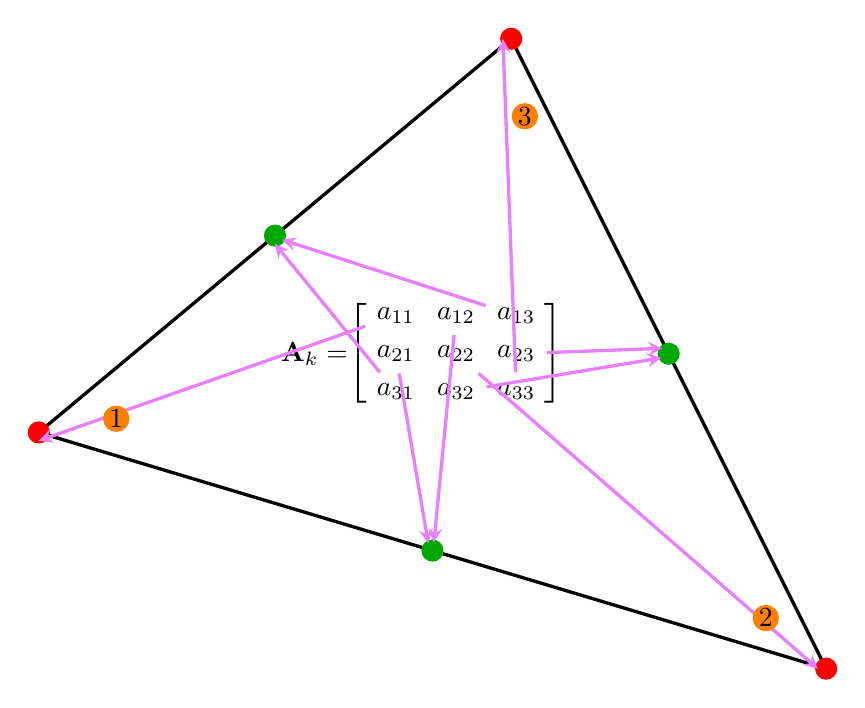
\begin{tikzpicture}	[>=stealth]
	
	\coordinate (A) at (0,3);
	\coordinate (B) at (10,0);
	\coordinate (C) at (6,8);
	\coordinate (D) at (5,1.5); % midpoint of AB
	\coordinate (E) at (8,4);   % midpoint of BC
	\coordinate (F) at (3,5.5); % midpoint of CA
	\coordinate (G) at (5.3,4); % center of gravity
	
	\draw[very thick] (A)--(B)--(C)--cycle;
	\fill[red] (A) circle (4pt) (B) circle (4pt) (C) circle (4pt);
	\fill[mid-green] (D) circle (4pt) (E) circle (4pt) (F) circle (4pt);
	

	\matrix [matrix of math nodes,	
	left delimiter={[},
	right delimiter={]},
	inner sep=-2pt,
	nodes={inner sep=.4em},
	](M) at (G) {
		a_{11} &a_{12} &a_{13}\\
		a_{21} &a_{22} &a_{23}\\
		a_{31} &a_{32} &a_{33}\\
	};
	
	
	\path (M.center)++(180:1.8cm) node {$\mathbf{A}_k=$};
	
	\draw[<-,line width=1.2pt,blue!20!magenta!50]
		(A)+(-90:3pt) -- (M-1-1);
	\draw[<-,line width=1.2pt,blue!20!magenta!50]
		(B)+(180:3pt) -- (M-2-2);
	\draw[<-,line width=1.2pt,blue!20!magenta!50]
		(C)+(180:3pt) -- (M-3-3);
		
	\draw[<-,line width=1.2pt,blue!20!magenta!50]
		(D)+(80:3pt) -- (M-1-2);
	\draw[<-,line width=1.2pt,blue!20!magenta!50]
		(D)+(120:3pt) -- (M-2-1);
	\draw[<-,line width=1.2pt,blue!20!magenta!50]
		(E)+(140:3pt) -- (M-2-3);
	\draw[<-,line width=1.2pt,blue!20!magenta!50]
		(E)+(210:3pt) -- (M-3-2);
	\draw[<-,line width=1.2pt,blue!20!magenta!50]
		(F)+(-30:3pt) -- (M-1-3);	
	\draw[<-,line width=1.2pt,blue!20!magenta!50]
		(F)+(-90:3pt) -- (M-3-1);
		
	
	\path
		(A)++(10:1cm) node[fill=orange,circle,inner sep=.5pt] {$1$}
		(B)++(140:1cm) node[fill=orange,circle,inner sep=.5pt] {$2$}
		(C)++(-80:1cm) node[fill=orange,circle,inner sep=.5pt] {$3$};
	
\end{tikzpicture}


		\caption{Cell-oriented assembly of Galerkin matrix by distribution
			from element matrices}
		\label{tikz:2D_cell-oriented_distribution_by_element_matrices}
	\end{figure}

	The green circles \greencircle{} can be regarded as the edges to which we 
	can associate the off-diagonal entries of the Galerkin matrix. An edge can 
	represent both $(\bA)_{ij}$ and $(\bA)_{ji}$, which accounts 
	for why there are two symmetric off-diagonal entries in an element matrix 
	contributing to an edge \greencircle{}. The algorithm describing the
	distribution scheme is given below.
	\begin{algorithm}[!htbp]
		\caption{Cell-oriented assembly of Galerkin matrix for
			linear finite elements}
		\label{alg:assembleGalerkinMatrix_cell-oriented}		
		\begin{algorithmic}[1]
	\State SparseMatrix $\mathbf{A}\in\mathbb{R}^{N,N},\ 
				N:=\sharp\mathcal{V}(\mathcal{M})$
	\State $\mathbf{A}:=\mathbf{0}$
	\State $M:=\sharp\mathcal{M}$ \Comment{no. of cells}
	\For{$i=1$ \textbf{to} $M$}
		\State $K\gets\mathtt{mesh.getElemCoords}(i)$ 
			\Comment{obtain cell-shape information}
		\State $\mathbf{A}_K\gets\mathtt{getElemMatrix}(K)$ 
			\Comment{compute element matrix, see 
				(\ref{eq:2D element (stiffness) matrix formula},~%
				 \ref{eq:2D element (stiffness) matrix component}) }
		\For{$k=1$ \textbf{to} $3$}
			\For{$j=1$ \textbf{to} $3$}
				\State $\mathbf{A}(i:\bx^i=\ba_K^k,\ell:\bx^\ell=\ba_K^j)\; 
					+\!\!= \mathbf{A}_K(k,j)$ \Comment{see Figure
				 \ref{tikz:2D_cell-oriented_distribution_by_element_matrices}}
			\EndFor
		\EndFor	
	\EndFor	
\end{algorithmic}

	\end{algorithm}	

	\subsubsection{Computation of Right-Hand Side Vector}
	Computation of the right-hand side vector $\vv{\bm{\varphi}}$, as one 
	possibly can guess, runs parallel to what we have studied in 
	Section \hyperref[subsubsection.2.2.3]{2.2.3}. We start from 
	the right-hand side linear form 
	\[\ell(v):=\int_{\Omega}f(\bx)v(\bx)\,\dx, \quad v\in H^1(\Omega),\ 
												f\in L^2(\Omega).\]
	From \eqref{eq:linear systems of equations formulas} we have learned that
	$\vv{\bm{\varphi}}=\left[\ell(b_h^j)\right]_{j=1}^{N}$, so we have
	\begin{equation}
		(\vv{\bm{\varphi}})_j=\ell(b_h^j)=\int_{\Omega}f(\bx)b_h^j(\bx)\,\dx,
			\quad j=1,...,N.
	\end{equation}
	
	Similarly, we split the right-hand side linear form into 
	\emph{cell contributions}:
	
	\vspace{10pt}
	\hspace{.07\textwidth}%
	\begin{minipage}{.3\textwidth}
		\centering
		\begin{equation*}
			(\vv{\bm{\varphi}})_j=\sum_{l=1}^{N_j}
				\int_{K_l}f(\bx)b_{h|K_l}^j(\bx)\,\dx,
		\end{equation*}
		where $K_1,...,K_{N_j}$ are the triangles adjacent to node $\bx_j$.
	\end{minipage}%
	\begin{minipage}{.5\textwidth}
		\centering
		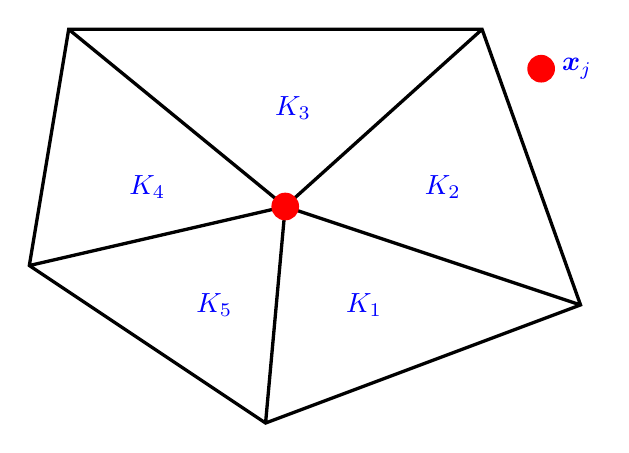
\begin{tikzpicture}	[>=stealth]
	
	\coordinate (A) at (3,0);
	\coordinate (B) at (7,1.5);
	\coordinate (C) at (5.75,5);
	\coordinate (D) at (.5,5);
	\coordinate (E) at (0,2);
	
	\coordinate (F) at (3.25,2.75); % the center, focus
	\coordinate (X) at (6.5,4.5);   % commentary node
	
	\draw[very thick] (A)--(B)--(C)--(D)--(E)--cycle
		(F)--(A) (F)--(B) (F)--(C) (F)--(D) (F)--(E);
	\fill[red] (F) circle (5pt)  (X) circle (5pt);	
	
	\path
		 (X)++(0:13pt) node[text=blue]{$\bx_j$}
		 (4.25,1.5) node[text=blue]{$K_1$} % (O1)
		 (5.25,3)   node[text=blue]{$K_2$} % (O2)
		 (3.35,4)   node[text=blue]{$K_3$} % (O3)
		 (1.5,3)    node[text=blue]{$K_4$} % (O4)
		 (2.35,1.5) node[text=blue]{$K_5$};% (O5)
	
\end{tikzpicture}

	\end{minipage}\\[8pt]
	
	Likewise on a single triangle $K\in\mathcal{M}$ we can define
	\begin{equation}
		\ell_K(b_h^j):=\int_K f(\bx)b_{h|K}^j(\bx)\,\dx=\ell_K(\lambda_i),
	\end{equation}
	where $\lambda_i$ is the barycentric coordinate function defined in
	\eqref{def:baraycentric coordinate function}. Thus we can rewrite 
	\begin{equation}
		(\vv{\bm{\varphi}})_j=\sum_{K,i:\ba_K^i = \bx_j}\ell_K(\lambda_i).
	\end{equation}

	To implement this sort of collecting scheme we would emulate the clumsy 
	and burdensome algorithm mentioned on page 
	\hyperref[alg:assembleGalerkinMatrix_vertex-centered]{16} somehow.	
	\begin{figure}[!htbp]
		\centering
		\input{input/tikz/2D_assemble_diagonal_element_vectors}
		% see https://www.texfaq.org/FAQ-extrabrace for \protect below
		\caption{$(\protect\vv{\bm{\varphi}})_j$ by summing diagonal entries
			of	element vectors of adjacent triangles}
		\label{tikz:2D_assemble_diagonal_element_vectors}
	\end{figure}\\
	But we have a better choice, that is to compute  $\vv{\bm{\varphi}}$
	in a cell-oriented fashion, in which way we end up with a counterpart 
	analogous to the element (stiffness) matrix from 
	\eqref{def:2D element (stiffness) matrix}, the 
	\begin{equation}\label{def:2D element (load) vector}
		\textrm{element (load) vector:}\quad \vv{\bm{\varphi}}_K := 
			\left[\ell_K(\lambda_i)\right]_{i=1}^3\in\mathbb{R}^3.
	\end{equation}\vspace{-20pt}
	\begin{figure}[!htbp]
		\centering
		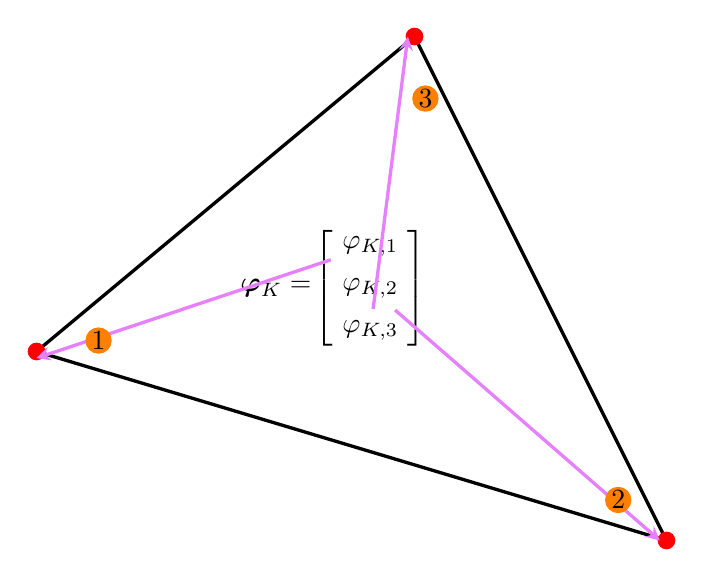
\begin{tikzpicture}	[>=stealth,scale=.8]
	
	\coordinate (A) at (0,3);
	\coordinate (B) at (10,0);
	\coordinate (C) at (6,8);
	\coordinate (G) at (5.3,4); % center of gravity
	
	\draw[very thick] (A)--(B)--(C)--cycle;
	\fill[red] (A) circle (4pt) (B) circle (4pt) (C) circle (4pt);	

	\matrix [matrix of math nodes,	
	left delimiter={[},
	right delimiter={]},
	inner sep=-2pt,
	nodes={inner sep=.4em},
	](M) at (G) {
		\varphi_{K,1}\\
		\varphi_{K,2}\\
		\varphi_{K,3}\\
	};	
	
	\path (M.center)++(180:1.5cm) node {$\vv{\bm{\varphi}}_K=$};
	
	\draw[<-,line width=1.2pt,blue!20!magenta!50]
		(A)+(-90:3pt) -- (M-1-1);
	\draw[<-,line width=1.2pt,blue!20!magenta!50]
		(B)+(180:3pt) -- (M-2-1);
	\draw[<-,line width=1.2pt,blue!20!magenta!50]
		(C)+(180:3pt) -- (M-3-1);			
	
	\path
		(A)++(10:1cm) node[fill=orange,circle,inner sep=.5pt] {$1$}
		(B)++(140:1cm) node[fill=orange,circle,inner sep=.5pt] {$2$}
		(C)++(-80:1cm) node[fill=orange,circle,inner sep=.5pt] {$3$};
	
\end{tikzpicture}


		\caption{Cell-oriented assembly of right-hand side vector by
			distribution from element vectors}
		\label{tikz:2D_cell-oriented_distribution_by_element_vectors}
	\end{figure}

	Now we consider how to compute $\vv{\bm{\varphi}}_K$. We know that in 1D,
	by trapezoidal rule, we can approximate $\int_a^b f(x)\,\rd x$ by 
	accumulating integrals on many small trapezoids. We can extend it to 2D:
	\begin{figure}[!htbp]
		\centering
		\begin{minipage}{.4\textwidth}
			\centering
			\includegraphics[width=1\linewidth]{svg/trapezoidal_rule_1D}
		\end{minipage}\quad$\longrightarrow$\quad
		\begin{minipage}{.5\textwidth}
			\centering
			\includegraphics[width=1\linewidth]{svg/integrate_on_a_triangle}
		\end{minipage}
	\end{figure}\\
	for triangle $K$ with vertices $\ba^1,\ba^2,\ba^3$
	\begin{equation}
		\int_{K}f(\bx)\,\dx\approx
			\frac{|K|}{3}\left(f(\ba^1)+f(\ba^2)+f(\ba^3)\right).
	\end{equation}
	Thus noting the cardinal basis property
	\eqref{pro:2D S_1^0(M) nodal (value) property} we obtain
	\begin{equation}\label{eq:2D element (load) vector formula}
		\vv{\bm{\varphi}}_K := \left[\ell_K(\lambda_i)\right]_{i=1}^3
		\approx \frac{|K|}{3}
		\begin{bmatrix}
			f(\ba^1)\\f(\ba^2)\\f(\ba^3)
		\end{bmatrix}.		
	\end{equation}
	This formula can be used for our computation of the element vector.
	The algorithm that assembles the right-hand side vector will be presented 
	in Section \hyperref[alg:assembleRhsVector]{4.3} in a more generic fashion.
		
%	\clearpage
	\section{Error Analysis}\label{section.3}
	A rigorous and complete analysis for the error estimates of finite element
	methods	is very complicated, which involves lots of techniques and 
	expertise. Therefore, here we will only show some conclusions that will be 
	used to	verify our numerical experiments in Section \ref{section.5} and 
	Section	\ref{subsection.6.4}. For more information about FEM error analysis 
	one	can refer to our text \cite[Section 2.2, 2.8]{LiRh} or this paper 
	\cite{FEMEA2005} by Thomas Gr\"{a}tsch and Klaus-J\"{u}rgen Bathe.\\
	
	\begin{mdframed}[linecolor=mid-green,linewidth=.5pt,roundcorner=10pt]
	For $p$-th order finite elements, the error measured in the $L^\infty$-norm 
	is of order $O(h^{p+1})$
	\[\norm{u-u_h}_{L^\infty(\Omega)}\leq Ch^{p+1}\norm{u},\]
	in the $L^2$-norm is of order $O(h^{p+1})$
	\[\norm{u-u_h}_{L^2(\Omega)}\leq Ch^{p+1}\norm{u},\]
	and in the $H^1$-norm is of order $O(h^{p})$
	\[\norm{u-u_h}_{H^1(\Omega)}\leq Ch^{p}\norm{u}.\]
	\end{mdframed}
	
	\clearpage
	\section{Implementation}\label{section.4}
	In this section, we discuss the nuts and bolts of the implementation of
	finite elements methods. However, implementing a robust, 
	industry-standard FEM library is a demanding job, requiring one to
	equip with not only a whole lot of mathematical skills but also 
	exceptional programming ability (especially strong background in 
	some compiled programming languages, like, C, C++, Fortran).
	The good news is that we don't have to implement one from scratch since 
	there are many well-established libraries out there now	which we can use 
	and learn from. Moreover, in practice, it is recommended that we use those 
	existing libraries to develop and deploy our own new algorithms for the 
	model problems we need to tackle as it can significantly reduce the 
	development cycle and save us from onerous debugging nightmares. So we are
	not going to implement a fully functional, versatile, and extensible FEM
	library. Instead, we will present a minimal implementation in the context
	of MATLAB, which makes our life easier by providing us with a tremendous
	number of built-in handy subroutines (functions), and most of all, as well
	as a powerful yet easy-to-use visualization system. But this doesn't mean 
	our implementation is trivial. We will cover many important aspects 
	concerning implementing a FEM library.
	
	In fact, many FEM libraries share similar frameworks and modules that 
	specify how the procedure goes and what results should be yielded in a 
	particular step.  Thus it makes sense to have a look at some successful
	FEM libraries, from which, at least ideawise, we can draw some 
	considerations.
			
	Hence, we start with looking at an industrial-strength
	open-source FEM library \href{https://dealii.org}{deal.II}, an outline of 
	how its primary groups of classes (main modules) interact is depicted in
	the following graph (simplified, omitted modules 
	PETSc, Trilinos, CUDA, UMFPACK for linear systems and linear 
	solvers): \vspace{-5pt}
	\begin{figure}[htbp!]
		\centering
		\includegraphics[width=0.6\linewidth]{svg/dealii_outline}
		\label{deal.ii outline}
	\end{figure}

	What we will discuss and try to implement is the 3rd level to the 5th level
	(top down). We shall first give some brief explanations to the modules in 
	the	above graph. For the detailed documentation one can refer to
	\url{https://www.dealii.org/current/doxygen/deal.II/index.html}.
	
	Mainfolds describe the shape of cells and, more generally, the geometry of 
	the domain on which one wants to solve an equation. The geometries can be
	obtained from the 3D modeling kernel OpenCASCADE via its APIs.
	
	Triangulation module does the meshing job that takes input from the
	geometries in Mainfold. This is usually done with the help of some
	external mesh generation libraries or tools, e.g. Gmsh. 
	
	Finite element classes describe the properties of a finite element space as 
	defined on the \emph{unit} cell. This includes, for example, how many 
	degrees of freedom are located at vertices, on lines, or in the interior of 
	cells. In addition, values and gradients of individual shape functions at 
	points on the unit cell are also of course provided. The DoFHandler class 
	allocates spaces so that each vertex, line, or cell of the triangulation 
	has the correct number of them. It also gives them a global numbering.
	
	The quadrature module is a set of rules that describe the location of 
	quadrature points on the unit cell, and the weights of quadrature points 
	thereon.
	
	Mapping classes make computing the matrix and right-hand side entries or 
	other quantities on each cell of a triangulation numerically practical by 
	mapping the shape functions, quadrature points, and quadrature weights from 
	the unit cell to each cell of a triangulation. The FEValues class is the 
	result of finite element shape functions and their gradients being 
	evaluated in quadrature points defined by a quadrature formula when mapped 
	to the real cell.
	
	After knowing the values and gradients of shape functions on individual 
	cells (by FEValues) and the global numbers of the degrees of freedom on a 
	cell (by DoFHandler), what we should do next is to assemble the system 
	matrix (and right hand side) of the linear system. This is done in the
	module Linear systems. Then we apply some appropriate solvers to solve
	this linear system of equations, which is followed by some post-processing
	visualization if one wants to.\vspace{8pt}
	
	We can clearly see that this outline largely agrees with what we have
	examined in Section \hyperref[section.2]{2}, but with more implementation
	details. Our own implementation will also cover these aspects though not
	in a very systematic way.   
	 	
	\subsection{Mesh Generation, Index Mapping, and Mesh Refinement}
	We will begin with triangulations which are fundamental to finite element
	methods. In industry, there are quite a number of choices to do the
	meshing job, a popular one is Gmsh, which is based around four modules:
	Geometry, Mesh, Solver and Post-processing, and it can be used at 3 levels:
	through the GUI, through the dedicated .geo language, through the C++, C,
	Python, and Julia API.\cite{Gmsh}
	
	Below is an example of Gmsh-constructed and -rendered geometry (mesh) 
	model. It can be expressed in a few lines of code in the highly-concise 
	.geo language, which can be found in
	\href{https://gitlab.onelab.info/gmsh/gmsh/blob/master/%
		demos/boolean/boolean.geo}{here}.
	\begin{figure}[!htbp]
		\centering
		\includegraphics[width=0.8\linewidth]{svg/boolean}
		\caption{A sphere after deleting 3 orthogonal cylinders from its center}
	\end{figure}

	\begin{minipage}{.2\textwidth}
		\includegraphics[width=1\linewidth]{
			svg/Delaunay_circumcircles_centers}
	\end{minipage}\hfill
	\begin{minipage}{.75\textwidth}
		\hspace{3ex}In MATLAB we can use its built-in \texttt{delaunay} 
		subroutine for mesh generation.
		The Delaunay triangulation, according to		
		\href{https://mathworld.wolfram.com/DelaunayTriangulation.html}{
			Wolfram MathWorld},	is a 
		\href{https://mathworld.wolfram.com/Triangulation.html}{triangulation} 
		which is equivalent to the
		\href{https://mathworld.wolfram.com/Nerve.html}{nerve} 
		of the cells in a 
		\href{https://mathworld.wolfram.com/VoronoiDiagram.html}{
			Voronoi diagram}, i.e., that triangulation of the 
		\href{https://mathworld.wolfram.com/ConvexHull.html}{convex hull} of 
		the points in the diagram in which every 
		\href{https://mathworld.wolfram.com/Circumcircle.html}{circumcircle}
		of a triangle is an empty circle.
	\end{minipage}
	
	The Computational Geometry Algorithms Library 
	(\href{https://www.cgal.org/}{CGAL}) which provides 
	easy access to efficient and reliable geometric algorithms
	also incorporates a bundle of 
	\href{https://doc.cgal.org/latest/Manual/packages.html%
		#PartTriangulationsAndDelaunayTriangulations}{
		triangulations and Delaunay triangulations} packages 
	along with a large number of other powerful data structures and 
	algorithms like
	\href{https://doc.cgal.org/latest/Manual/packages.html#PartVoronoiDiagrams}
	{Voronoi diagrams}, 
	\href{https://doc.cgal.org/latest/Manual/packages.html#PartPolyhedra}
	{cell complexes and polyhedra},
	\href{https://doc.cgal.org/latest/Manual/packages.html%
		#PartConvexHullAlgorithms}{convex hull algorithms},
	\href{https://doc.cgal.org/latest/Manual/packages.html%
		#PartSearchStructures}{spatial searching and sorting}, etc.	
	The mesh generator
	\href{http://persson.berkeley.edu/distmesh/}{DistMesh} that developed by 
	Per-Olof Persson and Gilbert Strang in the Department of Mathematics at 
	MIT is a good alternative as well in the context of MATLAB. \vspace{5pt}
	
	Now we observe the mesh quality generated by the MATLAB \texttt{delaunay}
	subroutine. For simplicity and comparison, we assume the computational 
	domain is a square and put the Gmsh counterpart by side. The results are 
	represented in the two figures below.\vspace{-10pt}	
	\begin{figure}[!htbp]
		\makebox[\textwidth][c]{
			\subfloat[A uniform triangular mesh generated via 
				MATLAB \texttt{delaunay}]
			{\includegraphics[width=0.3\linewidth]
				{svg/trimesh_matlab}} \qquad \qquad
			\subfloat[A somewhat random triangular mesh generated via Gmsh]
			{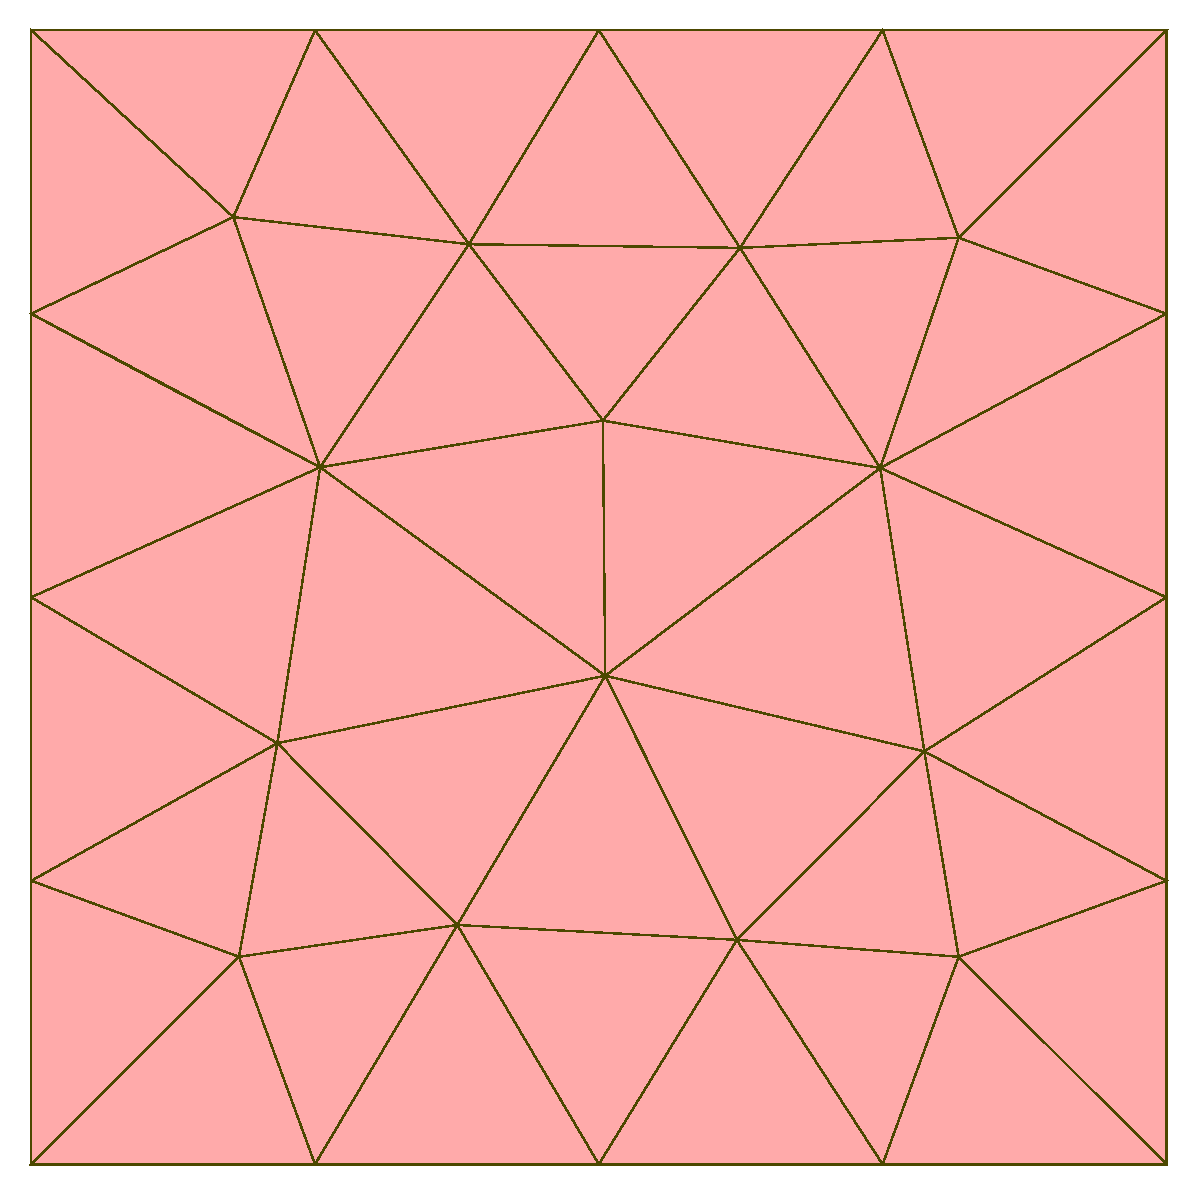
\includegraphics[width=0.3\linewidth]
				{svg/trimesh_gmsh}}
		}
	\end{figure}\\
	In fact, the subroutine \texttt{delaunay} takes two arguments in 2D with 
	syntax like this: \texttt{TRI = delaunay(X,Y)}. And we of course for 
	convenience chose to use the equidistant points as the input which led to
	the uniformly distributed triangular mesh. The Gmsh counterpart appears to 
	be somewhat random but with almost equally sized cells. It was generated 
	from the Gmsh GUI, possibly under the hood running some other algorithms in 
	the kernel. The MATLAB code for generating uniform triangular meshes on a
	rectangular region is given in Code listing \ref{code:generateMesh}.
	\vspace{-8pt}
	\begin{figure}[!htbp]
		\centering
		\hspace{.03\textwidth}%
		\begin{minipage}{0.7\textwidth}
			\centering
			\includegraphics[width=\linewidth]{
				svg/2D_index_mapping_by_dof_mapper}
		\end{minipage}%
		\begin{minipage}{0.27\textwidth}
			\centering
			\[\textcolor{blue}{\begin{array}{lccc}
				\sharp & \greencircled{1} & \greencircled{2} & 
				\greencircled{3} \\ \hline
				K_1  & 5  & 2  & 1\\
				K_2  & 3  & 5  & 2\\
				K_3  & 6  & 5  & 3\\
				K_4  & 4  & 8  & 9\\
				K_5  & 9  & 4  & 5\\
				K_6  & 5  & 9  & 6\\
				\rowcolor{pink} K_7  & 10 & 6  & 9\\
				K_8  & 10 & 7  & 6\\
				K_9  & 14 & 10 & 7\\
				K_{10} & 11 & 8  & 9\\
				K_{11} & 9  & 12 & 11\\
				K_{12} & 9  & 10 & 12\\
				K_{13} & 10 & 12 & 13\\
				K_{14} & 13 & 14 & 10\\
				K_{15} & 15 & 7  & 14\\
				K_{16} & 6  & 3  & 7\\
				K_{17} & 1  & 4  & 5
			\end{array}}\]
		\end{minipage}
		\caption{Index mapping by d.o.f. mapper}
		\label{fig:2D_index_mapping_by_dof_mapper}
	\end{figure}

	We have learned from Section \hyperref[section.2]{2} as well as the deal.II 
	library that the global node numbers and local vertex numbers are soooo
	important to the assembly of Galerkin matrices and right-hand side vectors.
	Hence, we zero in on the triangulation numbering and index mapping. 
	
	First, we consider the vertices (points/nodes). Simply enough we can use an 
	array for storing them, specifically, a \texttt{nP-by-nDim} array. That is,
	there are \texttt{nP} (number of points) rows and each row represents the 
	point's coordinates. In the 2D case, we can also use 3 columns to represent 
	the 2D coordinates leaving the 3rd column (coordinate of $z$) being 0. This 
	will comply with the 3D case. Thus to number the vertices we just need to 
	record their corresponding row numbers (indices). These numbers are 
	our global node numbers.
	
	Then, the elements of the mesh (triangles) can be represented by their
	corresponding vertex numbers (indices). Note that we also have to pay 
	attention to the local numbers. Hence we store an element in the order with 
	respect	to the local vertex numbers \greencircled{1}, \greencircled{2}, and 
	\greencircled{3}. This is illustrated in Figure 
	\ref{fig:2D_index_mapping_by_dof_mapper} and we call it index mapping by 
	d.o.f. mapper. Actually, this is also what \texttt{TRI = delaunay(X,Y)} is 
	done for us: it takes the points \texttt{(X,Y)} and creates a 2D Delaunay 
	triangulation represented by \texttt{TRI} which is a matrix of size 
	\texttt{mtri-by-3}, where \texttt{mtri} is the number of triangles. Each 
	row of \texttt{TRI} specifies a triangle defined by indices with respect to 
	the points.
	
	Mathematically, we can denote the local $\mapsto$ global index mapping 
	(d.o.f. mapper) by $\texttt{dofh}\in\mathbb{N}^{\sharp\mathcal{M},3}$
	with the meaning as follows:
	\begin{equation}\label{def:2D d.o.f. mapper dofh}
		\begin{array}{lll}
			\texttt{dofh}(k,l) & = & \textrm{global number of vertex } l 
			\textrm{ of } k\textrm{-th cell}\in \{1,...,N\},\\
			\bx_{\texttt{dofh}(k,l)}&=&\ba^l\textrm{ when }\ba^1,\ba^2,\ba^3
			\textrm{ are the vertices of } K_k,
		\end{array}
	\end{equation}
	for $l\in\{1,2,3\},\ k\in\{1,...,M\},\ M:=\sharp\mathcal{M},\ 
		N:=\sharp\mathcal{V}(\mathcal{M})$.
			
	\vspace{3pt}
	For example, the three vertices of the pink triangle $K_7$ in Figure 
	\ref{fig:2D_index_mapping_by_dof_mapper} can be represented with indices
	$\texttt{dofh}(7,1)=10,\ \texttt{dofh}(7,2)=6, \textrm{ and } 
	\texttt{dofh}(7,3)=9$, respectively.
	
	The d.o.f. mapper \texttt{dofh} as described in
	\eqref{def:2D d.o.f. mapper dofh} in a sense amounts to the 
	\texttt{DoFHandler} class in the deal.ii library, or rather it is a crude 
	and simple function that implements the index mapping.\vspace{5pt}
	
	Next we give a short discussion about mesh refinement. We know that the 
	accuracy of finite element methods is closely related to the mesh size
	$h_\mathcal{M}$. So naturally people would like to get finer meshes. We
	can achieve this by dividing the existing cells into sub-cells. Take the 
	triangular meshes for an example, one way is to add 3 more nodes at the 
	midpoints of the 3 edges of a cell and cut this triangle along these new 
	edges connected by the midpoints. Thus a triangular cell is divided into
	four congruent half-sized triangles.
	\begin{figure}[!htbp]
		\centering
		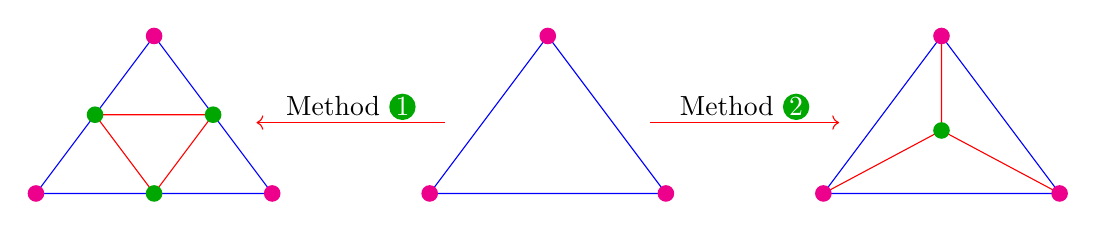
\begin{tikzpicture}			
	\draw[blue] (0,0)--(3,0)--(1.5,2)--cycle;			
	\draw[xshift=5cm,blue] (0,0)--(3,0)--(1.5,2)--cycle;
	\draw[xshift=10cm,blue] (0,0)--(3,0)--(1.5,2)--cycle;			
	\draw[red] (.75,1)--(2.25,1)--(1.5,0)--cycle;
	\draw[red,xshift=10cm] (1.5,.8)--(0,0)
						(1.5,.8)--(1.5,2) (1.5,.8)--(3,0);
	
	\foreach \m in {
		(0,0),(3,0),(1.5,2),
		(5,0),(8,0),(6.5,2),
		(10,0),(13,0),(11.5,2)} {				
		\fill[magenta] \m circle (3pt);
	}		
	\foreach \g in {
		(.75,1),(2.25,1),(1.5,0),(11.5,.8) } {				
		\fill[mid-green] \g circle (3pt);
	}
	
	\draw[<-,red] (2.8,.9) -- (5.2,.9);
	\draw[->,red,xshift=5cm] (2.8,.9) -- (5.2,.9);			
	
	\path (4,1.1) node{Method \greencircled{1}}
		++(0:5cm) node{Method \greencircled{2}};
\end{tikzpicture}

	\end{figure}
	
	Another approach for the triangular meshes is to add some node(s) inside 
	a cell, for instance, adding a new node in the barycenter of a triangle.
	Adding more than one inner point is also possible (e.g. adding one node
	in the barycenter then another node, again, at the barycenter of a divided 
	sub-triangle). In practice, the first approach is often adopted as it 
	creates regular/uniform finer meshes, which is usually desirable.	
	\begin{figure}[!htbp]
		\centering
		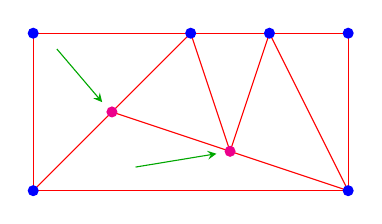
\begin{tikzpicture}[>=stealth]
	\draw[red] (0,0)--(4,0)--(4,2)--(0,2)--cycle;
	\draw[red] (0,0)--(2,2)--(2.5,.5)--(3,2)--(4,0)--(1,1);
	\foreach \p in {(0,0),(4,0),(4,2),(0,2),(2,2),(3,2)}
		\fill[blue] \p circle (2pt);
	\fill[magenta] (1,1) circle (2pt) (2.5,.5) circle (2pt);
	
	\draw[->,mid-green] (.3,1.8)--([shift=(135:5pt)]1,1);
	\draw[->,mid-green] (1.3,.3)--([shift=(190:5pt)]2.5,.5);
\end{tikzpicture}
	\end{figure}
	
	In the end, it should be emphasized that the triangulation or mesh 
	refinement should not contain or give rise to any ``hanging nodes", that 
	is it shouldn't violate the restriction that each triangle side (if not a 
	boundary edge) is entirely shared by two adjacent triangles (implied by 
	principle (iv) of triangulation as defined on page 
	\pageref{def:triangulation}).
		
	\subsection{Local Computations}\label{subsection.4.2}
	In Section \hyperref[subsubsection.2.2.3]{2.2.3} we have explored how to 
	compute the Galerkin matrix with omitting the diffusion coefficient 
	$\bm{\alpha}$ as well as the whole second term $\gamma(\bx)u$ in 
	\eqref{eq:PDE model} for the sake of simplicity. Now we add them back and 
	focus on the computation of the element matrix that corresponds to the 
	bilinear form 
	\[a(u,v)=\int_{\Omega}\bm{\alpha}(\bx)\grad u\cdot \grad v 
		+ \gamma(\bx) uv \,\dx,	\quad u,v\in H^1(\Omega). \]
	
	The element matrix for the above bilinear form is analogous to the one 
	presented in \eqref{def:2D element (stiffness) matrix}, that is
	\begin{equation}\label{def:2D reaction diffusion element matrix}
		\bA_K:=\left[a_K(\lambda_i,\lambda_j)\right]_{i,j=1}^3
			\in\mathbb{R}^{3,3},
	\end{equation}\vspace{-8pt}
	\begin{equation}\label{eq:2D reaction diffusion em formula}
		a_K(\lambda_i,\lambda_j)=\int_K\bm{\alpha}(\bx)\grad\lambda_i\cdot
		\grad\lambda_j+\gamma(\bx)\lambda_i \lambda_j\,\dx,
	\end{equation}
	where $\lambda_i, \lambda_j$ are the barycentric coordinate functions 
	defined in \eqref{def:baraycentric coordinate function}.  
	
	We start our investigation from a lemma below, which comes in handy in
	a few situations.
	\begin{lemma}[Integration of powers of barycentric coordinate 
				  functions {\cite[Lemma 2.7.5.5]{Hiptmair}}]
	For any non-degenerate $d$-simplex $K$ with barycentric coordinate
	functions $\lambda_1,...,\lambda_{d+1}$ and exponents
	$\alpha_j\in\mathbb{R}, j=1,...,d+1$,
	\[\int_{K}\lambda_1^{\alpha_1}\cdots\lambda_{d+1}^{\alpha_{d+1}}\,\dx
		= d!\,|K|\frac{\alpha_1!\,\alpha_2!\cdots\cdots\alpha_{d+1}!}{
		(\alpha_1+\alpha_2+\cdots+\alpha_{d+1}+d)! } \quad  
		\forall \bm{\alpha}\in\mathbb{R}^{d+1}.
	\]
	\end{lemma}

	A direct application of this lemma for now is to compute the element
	mass matrix 
	\[\bA_{K_M}:=\left[\int_K\lambda_i\lambda_j\,\dx\right]_{i,j=1}^3
			\in\mathbb{R}^{3,3}.\]	
	In fact, applying the above lemma with $d=2$ we immediately obtain 
	\begin{equation}
		\int_{K}\lambda_\ell(\bx)\,\dx = \frac{|K|}{3},\quad
		\int_{K}\lambda_\ell(\bx)^2\,\dx = \frac{|K|}{6},\quad
		\int_{K}\lambda_i(\bx)\lambda_j(\bx)\,\dx = \frac{|K|}{12},
	\end{equation}
	which suggest we can compute the element mass matrix by 
	\begin{equation}\label{eq:2D element (mass) matrix formula}
		\bA_{K_M}=\frac{|K|}{12}
		\begin{bmatrix}
			2 & 1 & 1\\
			1 & 2 & 1\\
			1 & 1 & 2
		\end{bmatrix}.
	\end{equation}
	
	Equipped with this formula we are now able to solve the following PDE
	model problem:
	\[-\Delta u + ku=f,\]
	where $k$ is a constant.
	
	Of course, all the stuff we have studied before will also be used.
	
	Woohoo! But wait a minute, what we get in here is an augmented version, 
	$\gamma(\bx)$ is not necessarily a constant, plus we have the scary first 
	term in \eqref{eq:2D reaction diffusion em formula} to handle, which 
	seems nontrivial at all.\vspace{5pt}
		
	Hence, we turn to an approximation technique called quadrature rules that 
	use weighted sum of	function values at specific points to approximate the
	definite integral of a function. And we call such a way of doing this on 
	an element $K\in\mathcal{M}$ a local quadrature rule, which can be 
	expressed as follows:
	\begin{equation}\label{eq:local quadrature rule}
		\int_K f(\bx)\,\dx \approx \sum_{l=1}^{P_K}\omega_l^K f(\bm{\xi}_l^K),
		\quad \bm{\xi}_l^K\in K,\,\omega_l^K\in\mathbb{R},\, P_K\in\mathbb{N}.
	\end{equation}
	Here, $\omega_l^K$ are the weights, $\bm{\xi}_l^K$ are the quadrature 
	points, and $P$ means $P$-point local quadrature rule.	
	
	Typically, these quadrature points defined by a quadrature formula are 
	known on \emph{reference elements}, that is, e.g. the unit interval 
	$[0,1]\in \mathbb{R}$ in 1D, the unit triangle \tikz \draw[magenta] 
	(0pt,0pt) -- (7pt,0pt) -- (0pt,7pt) -- cycle; connected by points 
	$(0,0),(1,0),(0,1)\in\mathbb{R}^2$ in 2D. Moreover, the function values
	and their gradients on a reference element can be rather easily computed.
	So an important step is to transform the quadrature points from the unit 
	cell (reference element) to a real cell of a mesh.	
	Then we are able to evaluate the function values and gradients on the real
	cells and subsequently compute 
	\eqref{eq:2D reaction diffusion em formula}. To achieve these we shall
	make a few preparations.
	
	\subsubsection*{Local Shape Functions}
	\bookmark[dest=\HyperLocalCurrentHref, level=3]{Local Shape Functions}
	First, we introduce an important notion appeared in the outline of 
	deal.ii library on page \pageref{deal.ii outline}, which is shape 
	functions. In fact, we have encountered shape functions at the very 
	beginning---the basis functions $b_h^i$ are actually also called global 
	shape functions (GSF)/global basis functions/degrees of freedom (DOFs).
	What we are currently interested in is the local shape functions, defined
	as below.
	\begin{mdframed}[linecolor=blue,linewidth=.5pt,roundcorner=10pt,%
		innertopmargin=0pt]
	\begin{definition}[Local shape functions (LSF)]\label{def:LSF}
		Given a finite element function space on a mesh $\mathcal{M}$ with 
		global shape functions $b_h^i,i=1,...,N$, for every mesh entity $K$
		we define 
		\[\{b_K^j\}_{j=1}^{Q(K)}:=\{b_{h|K}^j, K\subset\textrm{interior of 
			supp}(b_h^j)\}:=\textrm{set of local shape functions (LSF)},\]
		that is the local shape functions are the basis functions that cover
		$K$, restricted to $K$.
	\end{definition}
	\end{mdframed}
	
	Note that $Q(K)$ is the number of local shape functions on the cell $K$, 
	e.g. $Q(K)=3$ for a triangular cell and $Q(K)=4$ for a quadrilateral cell.
	
	It turns out that on a triangular mesh there are exactly 3 local shape 
	functions on each cell $K$, which indeed are the barycentric coordinate
	functions $\lambda_1,\lambda_2,\lambda_3$ introduced in Section 
	\hyperref[subsubsection.2.2.3]{2.2.3}.
		
	Below is an important example of local shape functions on the unit triangle 
	$\widehat{K}$ with vertices $
	\ba_{\widehat{K}}^1=\begin{bmatrix}0\\0\end{bmatrix},\ 
	\ba_{\widehat{K}}^2=\begin{bmatrix}1\\0\end{bmatrix},\ \textrm{and }
	\ba_{\widehat{K}}^3=\begin{bmatrix}0\\1\end{bmatrix}:$
	\vspace{-12pt}
	\begin{figure}[!htbp]
		\makebox[\textwidth][c]{
			\subfloat[$b_{\widehat{K}}^1(\bx):=1-x_1-x_2$]{
				\includegraphics[width=0.3\paperwidth]{
					svg/2D_unit_shape_function_1}}
			\subfloat[$b_{\widehat{K}}^2(\bx):=x_1$]{
				\includegraphics[width=0.3\paperwidth]{
					svg/2D_unit_shape_function_2}}
			\subfloat[$b_{\widehat{K}}^3(\bx):=x_2$]{
				\includegraphics[width=0.3\paperwidth]{
					svg/2D_unit_shape_function_3}}
		}
		\caption{Local shape functions on the unit triangle $\widehat{K}$}
		\label{fig:reference shape functions}
	\end{figure}
	
	We call the above local shape functions on the unit triangle (reference 
	element) $\widehat{K}$ \emph{reference shape functions} for the sake of 
	convenience. These reference shape functions are simple enough to
	evaluate their function values and gradients since their analytic
	formulas are directly known and are arguably the most straightforward
	affine linear functions in 2D.%\vspace{5pt}
	
	\subsubsection*{Affine Equivalence}
	\bookmark[dest=\HyperLocalCurrentHref, level=3]{Affine Equivalence}
	Next, we introduce the affine transformation of triangles and pullback of
	functions, both of which are very practical and useful.
	\begin{lemma}[Affine transformation of triangles 
							{\cite[Lemma 2.7.5.14]{Hiptmair}}]
	For any non-degenerate triangle $K\subset\mathbb{R}^2\ (|K|>0)$ with
	numbered vertices there is a unique affine transformation 
	$\bm{\Phi}_K,\ \bm{\Phi}_K(\widehat{\bx})=\mathbf{F}_K\widehat{\bx}+
	\bm{\tau}_K$, with $K=\bm{\Phi}_K(\widehat{K})$ and preserving the 
	numbering of the vertices.
	\end{lemma}
	
	This lemma tells us that all cells of a triangulation are affine images
	of the unit triangle $\widehat{K}$, see Figure 
	\ref{tikz:2D_affine_transformation_of_triangles} for an illustration.	
	For a general triangle $K$ with vertices 
	$\ba^1,\ba^2,\ba^3$, the affine mapping
	$\bm{\Phi}_K(\widehat{\bx}):=\mathbf{F}_K\widehat{\bx}+\bm{\tau}_K$
	can be set with 
	$\mathbf{F}_K:=\begin{bmatrix}\ba^2-\ba^1 & \ba^3-\ba^1\end{bmatrix},\ 
	\bm{\tau}_K:=\ba^1$, i.e.
	\begin{equation}\label{eq:affine transformation of triangles formula}
		\mathbf{F}_K:=
		\begin{bmatrix}
			a_1^2-a_1^1 & a_1^3-a_1^1\\
			a_2^2-a_2^1 & a_2^3-a_2^1
		\end{bmatrix}, \quad \bm{\tau}_K:=
		\begin{bmatrix}
			a_1^1\\
			a_2^1
		\end{bmatrix}.
	\end{equation}

	\begin{figure}[!htbp]
		\centering
		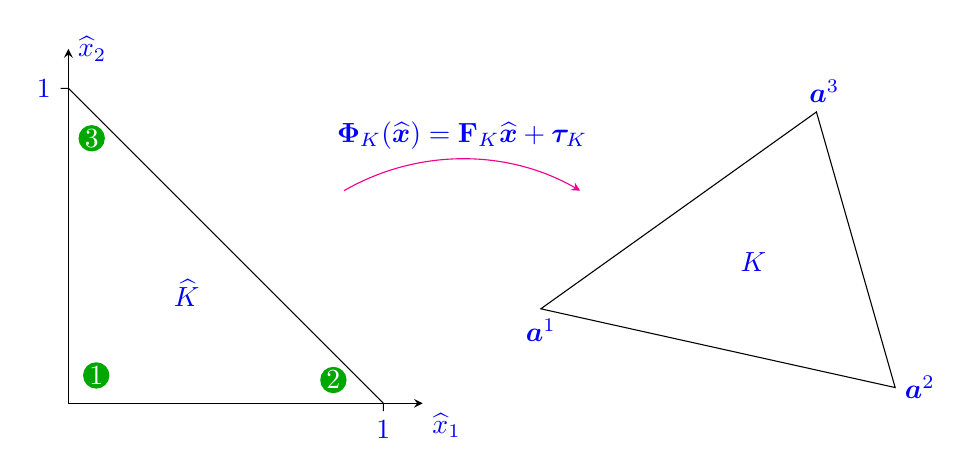
\begin{tikzpicture}[>=stealth]
	\draw[->] (0,0) -- (0,4.5);
	\draw[->] (0,0) -- (4.5,0);
	\draw (4,0)--(4,-.1) (0,4)--(-.1,4) (4,0)--(0,4);
	\path
		(4,-.1) node[anchor=north,text=blue]{$1$}
		(4.5,0) node[anchor=north west,text=blue]{$\widehat{x}_1$}
		(-.1,4) node[anchor=east,text=blue]{$1$}
		(0,4.5) node[anchor=west,text=blue]{$\widehat{x}_2$}
		(1.5,1.4) node[text=blue]{$\widehat{K}$}
		(0,0)++(45 :.5cm) node[text=white,fill=mid-green,circle, 
								inner sep=.5pt] {$1$}
		(4,0)++(155:.7cm) node[text=white,fill=mid-green,circle, 
								inner sep=.5pt] {$2$}
		(0,4)++(-65:.7cm) node[text=white,fill=mid-green,circle, 
								inner sep=.5pt] {$3$};
		
	\draw (6,1.2)--(10.5,.2)--(9.5,3.7) --cycle;
	
	\node[anchor=north,text=blue] at (6,1.2) {$\ba^1$};
	\node[anchor=west,text=blue] at (10.5,.2) {$\ba^2$};
	\node[anchor=south,text=blue] at (9.6,3.7) {$\ba^3$};
	\node[text=blue] at (8.7,1.8) {$K$};
	
	\draw[->,magenta] (3.5,2.7) arc (120:60:3cm);
	\node[text=blue] at (5,3.4) {
		$\bm{\Phi}_K(\widehat{\bx})=
			\mathbf{F}_K\widehat{\bx}+\bm{\tau}_K$};
	
\end{tikzpicture}

		\caption{The affine mapping $\bm{\Phi}_K$ that transforms
			 the unit triangle $\widehat{K}$ to a general triangle $K$}
		\label{tikz:2D_affine_transformation_of_triangles}
	\end{figure}

	\begin{mdframed}[linecolor=blue,linewidth=.5pt,roundcorner=10pt,%
		innertopmargin=0pt]
	\begin{definition}[Pullback]
		Given domains $\Omega,\widehat{\Omega}\subset\mathbb{R}^d$ and a 
		bijective mapping $\bm{\Phi}:\widehat{\Omega}\mapsto\Omega$, the 
		pullback $\bm{\Phi}^*u:\widehat{\Omega}\mapsto\mathbb{R}$ of a 
		function $u:\Omega\mapsto\mathbb{R}$ is a function defined on 
		$\widehat{\Omega}$ by	
		\[\bm{\Phi}^*u(\widehat{\bx}):=u(\bm{\Phi}(\widehat{\bx})),
			\quad \widehat{\bx}\in\widehat{\Omega}.\]
	\end{definition}
	\end{mdframed}

	What the definition above is saying can be visualized in the following 
	picture. \href{https://math.stackexchange.com/a/1189772}{Here} is also an 
	excellent explanation for pullback, which can be summarized as geometric 
	objects (e.g. points, vectors) ``go forward" and functions on them ``go 
	back".
	\begin{figure}[!htbp]
		\centering
		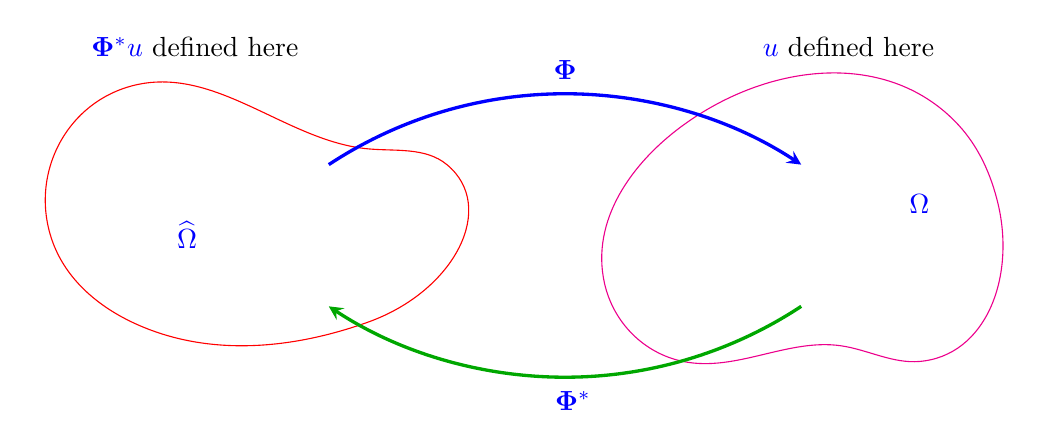
\begin{tikzpicture}[>=stealth]
	\foreach \x/\y/\z in 
	{0/1/a,1/3/b,4/2.2/c,5/2/d,4.5/.5/e,4/0/f,3/.2/g,1/0/h}{
		\coordinate (\z) at (\x,\y);
%		\fill[magenta] (\z)  circle (2pt) 
%		node[xshift=.3cm,text=blue] {$\z$};
	}
	
	\draw[use Hobby shortcut,closed=true,red]
	(a) .. (b) .. (c).. (d) .. (f) .. (h);
%	\draw [green] plot [smooth cycle] coordinates {
%	(a) (b) (c) (d) (f) (h)};
	
	\foreach \x/\y/\z in 
	{0/1/a,1/3/b,4/2.2/c,5/2/d,4.5/3/e,4/0/f,3/.2/g,1/0/h}{
		\coordinate [xshift=7cm,yshift=-.5cm](\z) at (\x,\y);
%		\fill[magenta] (\z)  circle (2pt) 
%		node[xshift=.3cm,text=blue] {$\z$};
	}
	\draw[use Hobby shortcut,closed=true,magenta]
	(a) .. (b) .. (e) ..  (d) .. (f) .. (g) .. (h);
	
	\draw[->,blue,very thick]
	(3.5,2) to [quick curve through={(6.5,2.9)}] (9.5,2);
	\draw[<-,mid-green,very thick]
	(3.5,.2) to [quick curve through={(6.5,-.7)}] (9.5,.2);
	
	\path 
		(6.5,3.2)  node[text=blue] {$\bm{\Phi}$}
	 	(6.6,-1)   node[text=blue] {$\bm{\Phi}^*$}
	 	(1.7,1.1)  node[text=blue] {$\widehat{\Omega}$}
	 	(11,1.5)   node[text=blue] {$\Omega$}
	 	(1.8, 3.5) node {\textcolor{blue}{$\bm{\Phi}^* u$} defined here}
	 	(10.1,3.5) node {\textcolor{blue}{$u$} defined here};
\end{tikzpicture}


	\end{figure}

	We're concerned with the pullback of local shape functions. Let 
	$K\in\mathcal{M},\widehat{K}$ be the unit triangle, and $\bm{\Phi}_K$ the
	unique affine mapping $\widehat{K}\mapsto K$, which respects the local 
	numbering of the vertices of $\widehat{K}$ and $K$:
	$\bm{\Phi}_K(\widehat{\ba}^i)=\ba^i,\ i=1,2,3$. We write 
	\begin{itemize}
		\item $b_K^1,b_K^2,b_K^3$ for the local shape functions on $K$, and
		\item $\widehat{b}^1,\widehat{b}^2,\widehat{b}^3$ for the local shape 	
			functions on $\widehat{K},$ i.e. reference shape functions (see
			Figure \ref{fig:reference shape functions}),
	\end{itemize}
	then we have a fundamental relationship in regard to the 
	pullback $\bm{\Phi}_K^*$:
	\begin{equation}\label{pro:pullback of local shape functions}
		\widehat{b}^i=\bm{\Phi}_K^* b_h^i \quad\Leftrightarrow\quad
		\widehat{b}^i(\widehat{\bx})=b_K^i(\bx),\quad
		\bx=\bm{\Phi}_K(\widehat{\bx}).
	\end{equation}

	This relationship is illustrated in Figure 
	\ref{tikz:2D_local_shape_function_mapping} which takes 
	$\widehat{b}^1\mapsto b_K^1$ for an example. A direct observation can
	be made	from the fact that $\widehat{b}^1(A)=b_K^1(A')=1,\ 
	\widehat{b}^1(B)=b_K^1(B')=\widehat{b}^1(C)=b_K^1(C')=0$. For a general
	case where the point $P\in\widehat{K}$,  and the transformed point 
	$P'=\bm{\Phi}_K(P)\in K$, all we have to do is notice a property that
	\href{https://en.wikipedia.org/wiki/Affine_transformation}{affine 
	transformation} possesses: it preserves the ratios of the lengths of 
	parallel line segments. Therefore,
	\[\frac{|EF|}{|BC|}=\frac{|E'F'|}{|B'C'|},\quad\Rightarrow\quad
	\frac{|AP|}{|AH|}=\frac{|A'P'|}{|A'H'|},\quad\Rightarrow\quad
	\frac{|PQ|}{|AD|}=\frac{|P'Q'|}{|A'D'|}.\]
	
	Note that $|AD|=|A'D'|=1$, thus we obtain 
	$\widehat{b}^i(P)=|PQ|=|P'Q'|=b_K^i(P')$, which proves
	\eqref{pro:pullback of local shape functions}.
	
	\begin{figure}[!htbp]
		\centering
		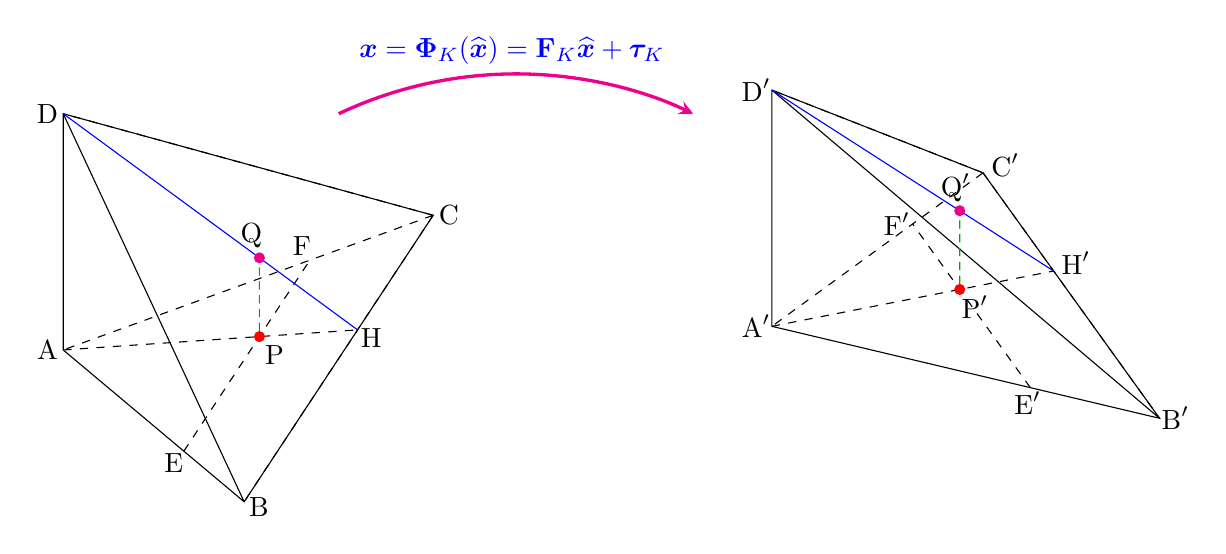
\begin{tikzpicture}[>=stealth]
	\coordinate (A) at (0,0);
	\coordinate (B) at (-40:3cm);
	\coordinate (C) at (20:5cm);
	\coordinate (D) at ($(A)+(90:3cm)$);
	
	\coordinate (E) at ($(A)!2/3!(B)$);
	\coordinate (F) at ($(A)!2/3!(C)$);
		
	\coordinate (H) at ($(B)!.6!(C)$);
	
	\draw (D)--(A)--(B)--(C)--cycle (D)--(B);
	\draw[dashed] (C)--(A) (C)--(B) (C)--(D);
	
	\draw[dashed] (E)--(F) (A)--(H);
	
	\fill[red] (intersection of A--H and E--F) coordinate (P) circle (2pt);
	\draw[blue] (D)--(H);
	
	\fill[magenta] (intersection of D--H and P--{$(P)+(90:3cm)$}) 
		coordinate (Q) circle (2pt);
	\draw[mid-green, densely dashed] ([yshift=2pt]P)--([yshift=-2pt]Q);
	
	\path
		(A)++(180:2mm) node {A}
		(B)++(-20:2mm) node {B}
		(C)++(  0:2mm) node {C}
		(D)++(180:2mm) node {D}
		(E)++(230:2mm) node {E}
		(F)++(120:2mm) node {F}
		(H)++(-30:2mm) node {H}
		(P)++(-50:3mm) node {P}
		(Q)++(110:3mm) node {Q};
	
%	=======================================

	\path[xshift=9cm] 
		(0,.3) coordinate (A1)
		(-10:5cm) coordinate (B1)
		(40:3.5cm) coordinate (C1)
		($(A1)+(90:3cm)$) coordinate (D1);
	
	\coordinate (E1) at ($(A1)!2/3!(B1)$);
	\coordinate (F1) at ($(A1)!2/3!(C1)$);
	
	\coordinate (H1) at ($(B1)!.6!(C1)$);
	
	\draw (D1)--(A1)--(B1)--(C1)--cycle (D1)--(B1);
	\draw[dashed] (C1)--(A1) (C1)--(B1) (C1)--(D1);
	
	\draw[dashed] (E1)--(F1) (A1)--(H1);
	
	\fill[red] (intersection of A1--H1 and E1--F1) coordinate (P1) circle (2pt);
	\draw[blue] (D1)--(H1);
	
	\fill[magenta] (intersection of D1--H1 and P1--{$(P1)+(90:3cm)$}) 
		coordinate (Q1) circle (2pt);
	\draw[mid-green, densely dashed] ([yshift=2pt]P1)--([yshift=-2pt]Q1);
	
	\path
		(A1)++(180:2mm) node {$\textrm{A}'$}
		(B1)++(  0:2mm) node {$\textrm{B}'$}
		(C1)++( 20:3mm) node {$\textrm{C}'$}
		(D1)++(180:2mm) node {$\textrm{D}'$}
		(E1)++(260:2mm) node {$\textrm{E}'$}
		(F1)++(180:2mm) node {$\textrm{F}'$}
		(H1)++( 20:3mm) node {$\textrm{H}'$}
		(P1)++(-50:3mm) node {$\textrm{P}'$}
		(Q1)++(100:3mm) node {$\textrm{Q}'$};
		
	\draw[->,magenta,very thick]
		(3.5,3) to [quick curve through={(6,3.5)}] (8,3);
	\node[text=blue] at (5.7,3.8) {
		$\bx=\bm{\Phi}_K(\widehat{\bx})=
			\mathbf{F}_K\widehat{\bx}+\bm{\tau}_K$};	
\end{tikzpicture}


		\caption{
			\centering
			The affine mapping $\bm{\Phi}_K$ preserves the values of local 
			shape functions:
			\begin{minipage}{\linewidth}
				\[P\in \widehat{K}, P'=\bm{\Phi}_K(P)\in K,\quad
				\Rightarrow\quad\widehat{b}^i(P)=|PQ|=|P'Q'|=b_K^i(P').\]
			\end{minipage}
		}
		\label{tikz:2D_local_shape_function_mapping}
	\end{figure}
 
	\subsubsection*{Local Quadrature}
	\bookmark[dest=\HyperLocalCurrentHref, level=3]{Local Quadrature}	
	With the above preliminaries we are now all set for the final work
	of computing the element matrix in 
	(\ref{def:2D reaction diffusion element matrix},~%
	 \ref{eq:2D reaction diffusion em formula}). Let's dive in.
	
	We write $\bm{\Phi}_K(\widehat{\bx}):=\mathbf{F}_K\widehat{\bx}+
	\bm{\tau}_K$ for the affine transformation from the reference triangle
	$\widehat{K}$ to the general triangle $K$. By the transformation formula 
	for integrals we can pull back integrals over $K$ to $\widehat{K}$:
	\begin{equation}
		\int_{K} f(\bx)\,\dx=\int_{\widehat{K}} f(\bm{\Phi}_K(\widehat{\bx}))
		\,|\,\mathrm{det}\,\mathbf{F}_K\,|\,\rd\widehat{\bx}.
	\end{equation}
	Combining this formula with \eqref{eq:local quadrature rule} yields
	\begin{equation}\label{eq:transformed quadrature rule}
		\int_{K} f(\bx)\,\dx\approx|\,\mathrm{det}\,\mathbf{F}_K\,|\,
		\sum_{l=1}^{P}\widehat{\omega}_l\,f(\bm{\Phi}_K(\widehat{\bm{\xi}}_l)).
	\end{equation}
	
	The above formulas can be used for computing the element reaction matrix 
	(the second term) in \eqref{eq:2D reaction diffusion em formula}:
	\begin{align}
		&\int_{K} \gamma(\bx)\,\underbrace{\lambda_i(\bx)}_{=\,b_K^i(\bx)}\,
		\underbrace{\lambda_j(\bx)}_{=\,b_K^j(\bx)}\,\dx \nonumber \\ 
		=\;&\int_{\widehat{K}} \gamma(\bm{\Phi}_K(\widehat{\bx}))\,
		\underbrace{b_K^i(\bm{\Phi}_K(\widehat{\bx}))}_{\textrm{by 
		\eqref{pro:pullback of local shape functions}, }=\,
			\widehat{b}^i(\widehat{\bx}) }\,
		\underbrace{b_K^j(\bm{\Phi}_K(\widehat{\bx}))}_{=\,
			\widehat{b}^j(\widehat{\bx}) }\,
		|\,\mathrm{det}\,\mathbf{F}_K\,|\,\rd\widehat{\bx} \nonumber \\ 
		=\;&|\,\mathrm{det}\,\mathbf{F}_K\,|\,
		\sum_{l=1}^{P}\widehat{\omega}_l\,
		\gamma(\bm{\Phi}_K(\widehat{\bm{\xi}}_l))\,
		\widehat{b}^i(\widehat{\bm{\xi}}_l)\,
		\widehat{b}^j(\widehat{\bm{\xi}}_l).%
		\label{eq:element reaction matrix quadrature formula}
	\end{align}	
	Here, $\bm{\Phi}_K(\widehat{\bm{\xi}}_l), l=1,...,P$ are the transformed 
	quadrature points, which together with $|\mathrm{det}\,\mathbf{F}_K|$
	can be computed by \eqref{eq:affine transformation of triangles formula},
	and the reference shape functions values 
	$\widehat{b}^i(\widehat{\bm{\xi}}_l), i=1,2,3, l=1,...,P$ on the 
	quadrature points $\widehat{\bm{\xi}}_l$ defined on $\widehat{K}$ can 
	be precomputed by \texttt{[1-x1-x2,x1,x2]} with \texttt{(x1,x2)} 
	being these quadrature points. 
	
	The element vector \eqref{def:2D element (load) vector} 
	can also be computed thus:
	\begin{align}
		(\vv{\bm{\varphi}}_K)_i = \int_{K} f(\bx) b_K^i(\bx)\,\dx
		&=\int_{\widehat{K}} f(\bm{\Phi}_K(\widehat{\bx}))\,
		\widehat{b}^i(\widehat{\bx})\,
		|\,\mathrm{det}\,\mathbf{F}_K\,|\,\rd\widehat{\bx} \nonumber \\
		&=|\,\mathrm{det}\,\mathbf{F}_K\,|\,
		\sum_{l=1}^{P}\widehat{\omega}_l\,
		f(\bm{\Phi}_K(\widehat{\bm{\xi}}_l))\,
		\widehat{b}^i(\widehat{\bm{\xi}}_l).%
		\label{eq:2D element vector quadrature formula}
	\end{align}	
	See Code listing \ref{code:assembleVectorByGaussQuad} for its MATLAB 
	implementation.%\vspace{5pt}
	
	So, now there is only the first term (the element diffusion matrix) in 
	\eqref{eq:2D reaction diffusion em formula} left. Let's zero in on it.
	This time we will write $f(\bm{\Phi}_K(\widehat{\bx}))$ as the pullback
	form $(\bm{\Phi}_K^* f)(\widehat{\bx})$, then
	\begin{align}
		&\int_{K}\bm{\alpha}(\bx)\grad b_K^i(\bx)\cdot\grad b_K^j(\bx)\,\dx
		\nonumber \\
		=\;&\int_{\widehat{K}}
		(\textcolor{mid-green}{\bm{\Phi}_K^*}\bm{\alpha})(\widehat{\bx})
		(\underbrace{\textcolor{mid-green}{\bm{\Phi}_K^*}
			(\grad b_K^i)}_{\textcolor{red}{=\,?}})(\widehat{\bx})\cdot
		(\underbrace{\textcolor{mid-green}{\bm{\Phi}_K^*}
			(\grad b_K^j)}_{\textcolor{red}{=\,?}})(\widehat{\bx})\,
		|\,\mathrm{det}\,\mathrm{D}\bm{\Phi}_K(\widehat{\bx})\,|\,
		\rd\widehat{\bx}.\label{eq:vexing gradients}
	\end{align}
	
	The vexing problem is how do we compute the \textcolor{red}{$=\,?$} parts
	in \eqref{eq:vexing gradients}? The local shape functions $b_K^i$, (affine)
	linear functions though, are sort of elusive. One may think of using the 
	brute-force way of doing it, that is to calculate the analytic formulas
	(planes) of the local shape functions on the general triangle $K$, and 
	consequently their gradients can be computed. This sounds not that scary, 
	huh? Well, but actually we don't have to do so. The following lemma leads
	to a cleaner and faster solution.
	\begin{lemma}[Transformation formula for gradients
		{\cite[Lemma 2.8.3.10]{Hiptmair}}]
	For differentiable $u:K\mapsto\mathbb{R}$ and any 
	\href{https://en.wikipedia.org/wiki/Diffeomorphism}{diffeomorphism}
	$\bm{\Phi}:\widehat{K}\mapsto K$ we have
	\[(\mathbf{grad}_{\widehat{\bx}}(\bm{\Phi}^* u))(\widehat{\bx})=
	(\mathrm{D}\bm{\Phi}(\widehat{\bx}))^\top
	\underbrace{(\mathbf{grad}_{\bx} u)(\bm{\Phi}(\widehat{\bx}))}_{
	=\bm{\Phi}^* (\grad u)(\widehat{\bx}) }
	\quad \forall \widehat{\bx}\in\widehat{K}. \]	
	\end{lemma}
	\begin{proof}
	By the \emph{chain rule} the components of the gradient vector become
	\[(\grad\bm{\Phi}^* u(\widehat{\bx}))_i = \frac{\partial\bm{\Phi}^* u}{
	\partial\widehat{x}_i}(\widehat{\bx}) = 
	\frac{\partial}{\partial\widehat{x}_i} u (\bm{\Phi}(\widehat{\bx}))=
	\sum_{j=1}^{d}\frac{\partial u}{\partial x_j} (\bm{\Phi}(\widehat{\bx}))
	\frac{\partial\bm{\Phi}_j}{\partial\widehat{x}_i}(\widehat{\bx}),
	\]
	then in the vector form we have
	\[
	\begin{bmatrix}
		\dfrac{\partial\bm{\Phi}^* u}{\partial\widehat{x}_i}(\widehat{\bx})\\
		\vdots\\
		\dfrac{\partial\bm{\Phi}^* u}{\partial\widehat{x}_d}(\widehat{\bx})
	\end{bmatrix}=
	(\mathbf{grad}_{\widehat{\bx}}(\bm{\Phi}^* u))(\widehat{\bx})=
	(\mathrm{D}\bm{\Phi}(\widehat{\bx}))^\top
	\begin{bmatrix}
		\dfrac{\partial u}{\partial x_i}(\bm{\Phi}(\widehat{\bx}))\\		
		\vdots\\
		\dfrac{\partial u}{\partial x_d}(\bm{\Phi}(\widehat{\bx}))
	\end{bmatrix}=
	(\mathrm{D}\bm{\Phi}(\widehat{\bx}))^\top
	(\mathbf{grad}_{\bx} u)(\bm{\Phi}(\widehat{\bx})).\]
	%
	Here, $\mathrm{D}\bm{\Phi}(\widehat{\bx})\in\mathbb{R}^{d,d}$ is the 
	Jacobian of $\bm{\Phi}$ at $\widehat{\bx}\in\widehat{K}$, the general 
	formula for Jacobian matrix is
	%
	\[\mathrm{D}\bm{f}(\bx)=\left[\frac{\partial f_i}{\partial x_j}
	\right]_{i,j=1}^{m,n} = 
	\begin{bmatrix}
		\dfrac{\partial f_1}{\partial x_1}(\bx) & \cdots & 
		\dfrac{\partial f_1}{\partial x_n}(\bx)\\
		\vdots &\ddots &\vdots \\
		\dfrac{\partial f_m}{\partial x_1}(\bx) & \cdots &
		\dfrac{\partial f_m}{\partial x_n}(\bx)
	\end{bmatrix} \in\mathbb{R}^{m,n}
	\]
	\end{proof}
	
	Therefore, by using the above lemma we arrive at
	\begin{align}
		&\int_{K}\bm{\alpha}(\bx)\grad b_K^i(\bx)\cdot\grad b_K^j(\bx)\,\dx
		\nonumber \\
		=\;&\int_{\widehat{K}}
		\bm{\alpha}(\bm{\Phi}_K(\widehat{\bx}))
		\left((\mathrm{D}\bm{\Phi}_K(\widehat{\bx}))^{-\top}
		\mathbf{grad}_{\widehat{\bx}}\widehat{b}^i(\widehat{\bx})\right)\cdot 
		\left((\mathrm{D}\bm{\Phi}_K(\widehat{\bx}))^{-\top}
		\mathbf{grad}_{\widehat{\bx}}\widehat{b}^j(\widehat{\bx})\right)\,
		|\,\mathrm{det}\,\mathrm{D}\bm{\Phi}_K(\widehat{\bx})\,|\,
		\rd\widehat{\bx} \nonumber \\	
		=\;&\sum_{l=1}^{P}\widehat{\omega}_l\,
		\bm{\alpha}(\bm{\Phi}_K(\widehat{\bm{\xi}}_l))
		\left((\mathrm{D}\bm{\Phi}_K(\widehat{\bm{\xi}}_l))^{-\top}
		\grad\widehat{b}^i(\widehat{\bm{\xi}}_l)\right)\cdot 
		\left((\mathrm{D}\bm{\Phi}_K(\widehat{\bm{\xi}_l}))^{-\top}
		\grad\widehat{b}^j(\widehat{\bm{\xi}}_l)\right)\,
		|\,\mathrm{det}\,\mathrm{D}\bm{\Phi}_K(\widehat{\bm{\xi}}_l)\,|\\
		=\;&|\,\mathrm{det}\,\mathbf{F}_K\,|\,
		\sum_{l=1}^{P}\widehat{\omega}_l\,
		\bm{\alpha}(\bm{\Phi}_K(\widehat{\bm{\xi}}_l))
		\left(\mathbf{F}_K^{-\top}
		\grad\widehat{b}^i(\widehat{\bm{\xi}}_l)\right)\cdot 
		\left(\mathbf{F}_K^{-\top}
		\grad\widehat{b}^j(\widehat{\bm{\xi}}_l)\right).%
		\label{eq:element diffusion matrix quadrature formula}
	\end{align}
	
	Terrific! The formula 
	\eqref{eq:element diffusion matrix quadrature formula} 
	for the entries of the element diffusion matrix is totally
	manageable! And in the linear finite element method, the gradients of
	the reference shape functions $\widehat{b}^1,\widehat{b}^2,\widehat{b}^3$
	are ever straightforward---they are constants which can be written as
	\texttt{[-1 -1;1 0;0 1]} in MATLAB. The MATLAB implementation for computing 
	the element matrix (\ref{def:2D reaction diffusion element matrix},~%
	\ref{eq:2D reaction diffusion em formula}) is given in Code listing 
	\ref{code:assembleReactionDiffusionMatrix}.	
	
	\subsection{Assembly Algorithms}
	Now we present the generic assembly algorithms for the Galerkin matrix
	and the right-side vector with introducing an abstract ``d.o.f. mapper/%
	handler" facility \texttt{locglobmap}, defined as follows:
	\[\texttt{locglobmap}(K,i) = j,\quad \textrm{if } b_{h|K}^j = b_K^i,
		\quad i=\{1,...,Q(K)\}.\]
	
	Note that according to Definition \ref{def:LSF} every mesh entity 
	$K$ is also endowed with a set of local shape functions 
	$\{b_K^1,...,b_K^{Q(K)}\}$, not merely cells.
	
	The \texttt{locglobmap} can be deemed as the generalized version of
	\texttt{dofh} introduced in \eqref{def:2D d.o.f. mapper dofh}, with
	a relationship by
	\[\texttt{dofh}(k,l)=\texttt{locglobmap}(K,l),\quad
		\textrm{if $K$ has index $k$},	\quad l\in\{1, 2, 3\}.\] 
	
	The abstract algorithms are given below. Typically, on a triangular mesh 
	$Q(K)\equiv3$ holds for all mesh entities $K\in\mathcal{M}$.
	\begin{algorithm}[!htbp]
		\caption{Abstract assembly routine for finite element Galerkin matrices}
		\label{alg:assembleGalerkinMatrix}
		\begin{algorithmic}[1]		
	\Procedure{assembleGalerkinMatrix}{Mesh $\mathcal{M}$}
	\State $\mathbf{A}=N\times N$ sparse matrix		
				\Comment{allocate zero sparse matrix}
	\ForAll{$K\in \mathcal{M}$} \Comment{loop over all cells}
		\State $Q(K)=\texttt{no\_loc\_shape\_functions}(K)$
		\State $\mathbf{A}_K=\texttt{getElementMatrix}(K)$
			\Comment{compute element matrix, see 
				(\ref{eq:2D element (stiffness) matrix formula},~%
				 \ref{eq:2D element (stiffness) matrix component},~%
				 \ref{eq:2D element (mass) matrix formula})/%
				(\ref{eq:element reaction matrix quadrature formula},~%
				 \ref{eq:element diffusion matrix quadrature formula}) }
		\State Vector $ idx = \{\texttt{locglobmap}(K,1),..., 
				\texttt{locglobmap}(K,Q(K))\}$ \Comment{get global indices}
		\For{$i=1$ \textbf{to} $Q(K)$}
			\For{$j=1$ \textbf{to} $Q(K)$}
				\State $\mathbf{A}(idx(i),idx(j))\; +\!\!=
					\mathbf{A}_K(i,j)$ \Comment{see Figure
				\ref{tikz:2D_cell-oriented_distribution_by_element_matrices}}
		\EndFor
		\EndFor
	\EndFor
	\State \Return $\mathbf{A}$
	\EndProcedure
\end{algorithmic}
	\end{algorithm}
	
	\begin{algorithm}[!htbp]
		\caption{Generic assembly algorithm for finite element R.H.S. vectors}
		\label{alg:assembleRhsVector}
		\begin{algorithmic}[1]		
	\Procedure{assembleRhsVector}{Mesh $\mathcal{M}$}
	\State $\vv{\bm{\varphi}} =	\textrm{Vector}(N)$		
				\Comment{preallocate appropriate memory}
	\ForAll{$K\in \mathcal{M}$} \Comment{loop over all cells}
		\State $Q(K)=\texttt{no\_loc\_shape\_functions}(K)$
		\State $\vv{\bm{\varphi}}_K=\texttt{getElementVector}(K)$
			\Comment{compute element vector, see 
				\eqref{eq:2D element (load) vector formula}/%
				\eqref{eq:2D element vector quadrature formula}}
		\State Vector $ idx = \{\texttt{locglobmap}(K,1),..., 
				\texttt{locglobmap}(K,Q(K))\}$ \Comment{get global indices}
		\For{$i = 1$ \textbf{to}  $Q(K)$}		
			\State $\vv{\bm{\varphi}}(idx(i))=\vv{\bm{\varphi}}(idx(i))+
					\vv{\bm{\varphi}}_K(i)$
			\Comment{see Figure 
				\ref{tikz:2D_cell-oriented_distribution_by_element_vectors}}
		\EndFor
	\EndFor
	\State \Return $\vv{\bm{\varphi}}$
	\EndProcedure
\end{algorithmic}
	\end{algorithm}
	
	\subsection{Incorporation of Boundary Conditions}
	Up to this point, we have finished the local computations of the element 
	Galerkin matrix and the element vector as well as the assembly process.
	Thus there is only one thing left before we solve the linear system of 
	equations, that is the imposition of boundary conditions. Here we will 
	focus on two kinds of boundary conditions: Dirichlet boundary conditions
	and Neumann boundary conditions, the former of which are also referred to 
	as \emph{essential} boundary conditions because they are directly imposed 
	on trial space and (in homogeneous form) on test space, and the latter of
	which are also referred to as \emph{natural} boundary conditions because 
	they are enforced only through the variational equation (the Neumann 
	boundary conditions ``naturally" emerge when removing constraints on the 
	boundary).
	
	In Section \ref{section.1} we considered the simplest homogeneous Neumann 
	problem for the purpose of developing the Galerkin discretization strategy 
	with relative ease. Now we first examine the non-homogeneous Neumann 
	boundary value problem
	\begin{equation}
		\begin{array}{rl}
			-\nabla\cdot(\bm{\alpha}(\bx) \nabla u)+
			\gamma(\bx)u=f, &\textrm{in }\Omega,\\
			\bm{\alpha}(\bx)\nabla{u}\cdot\bm{n}=g_n,
			&\textrm{on }\partial\Omega.
		\end{array}
	\end{equation}
	The corresponding variational formulation is 
	\begin{equation}
		u\in H^1(\Omega):\ 
		\int_{\Omega}\left(\bm{\alpha}(\bx)\nabla u\cdot\nabla v+
			\gamma(\bx)uv\right)\dx = 
		\int_{\Omega}fv\,\dx + \int_{\partial\Omega} g_n v\,\rd s 
		\quad\forall v\in H^1(\Omega).
	\end{equation}
	Substituting the test function $v$ with \eqref{eq:linear combi of v_h} the 
	right-hand side becomes
	\begin{equation}
		\int_{\Omega}fv_h\,\dx + \int_{\partial\Omega} g_n v_h\,\rd s =
		\sum_{i=1}^{N}\nu_i\left[\ell(b_h^i)+
		\int_{\partial\Omega}g_n b_h^i\,\rd s \right].
	\end{equation}
	\vspace{-15pt}
	\begin{figure}[!htbp]
		\begin{minipage}{.2\textwidth}
			\includegraphics[width=1\linewidth]{svg/boundary_triangles}
		\end{minipage}%
		\begin{minipage}{.8\textwidth}
			\hspace{3ex}Hence, compared to the right-hand side vector derived 
			in (\ref{eq:Galerkin weak problem}--%
			\ref{eq:linear systems of equations formulas}) we just need to add 
			$\int_{\partial\Omega}g_n b_h^i\,\rd s$ to each component of the 
			right-hand side vector $\vv{\bm{\varphi}}$. Note that 
			$\int_{\partial\Omega}g_n b_h^i\,\rd s$	is non-zero only when the 
			vertex $\bx_i$ is on the boundary $\partial\Omega$, therefore only 
			the additions to the components whose indices are the global node 
			numbers of boundary vertices are required, in which cases the 
			additions become			
		\end{minipage}
	\end{figure}
	\vspace{-10pt}
	\begin{equation}\label{eq:addition on boundary dofs of RHS}
		\Delta\vv{\bm{\varphi}}_i=
		\int_{\partial\Omega}g_n b_h^i\,\rd s=
		\int_{e_1}+\int_{e_2} g_n b_h^i\,\rd s,\quad 
		e_1,e_2\in\mathcal{E}_B(\mathcal{M}),\,
		e_1\cap e_2 = \bx_i\in\mathcal{V}_B(\mathcal{M}).
	\end{equation}
	These contributions can also be computed by cell-oriented or rather 
	(boundary) edge-oriented assembly on $\mathcal{M}_{|\partial\Omega}$, that
	is we traverse each boundary cell $K$/edge $e$ and then distribute the 
	cell contribution to the two vertices of the edge $e$. Note that on 
	each boundary cell $K$ only the two local shape functions whose nodal 
	values are over the two vertices of the edge $e$ do have contributions.
	
	To implement this one must at least provide a facility or a mesh data 
	structure that enables us to loop over the boundary edges of a particular
	type (Neumann, Dirichlet, Robin, etc). The Nektar++ framework which uses 
	XML to specify the boundary conditions by tags and values \cite{Netkar++}
	is a great resource that we can learn from.
	
	Next, consider the non-homogeneous Dirichlet boundary value problem
	\begin{align}
		-\nabla\cdot(\bm{\alpha}(\bx) \nabla u)+
		\gamma(\bx)u=f, \quad &\textrm{in }\Omega,
		\label{eq:Dirichlet PDE} \\
		u=g_d, \quad &\textrm{on }\partial\Omega,
		\label{eq:non-homogeneous Dirichlet BC}
	\end{align}
	with variational formulation
	\begin{equation}\label{eq:Dirichlet variational formulation}
		\begin{array}{l}			
			u\in H^1(\Omega)\\
			u=g_d \textrm{ on }\partial\Omega
		\end{array}:\ 
		\int_{\Omega}\left(\bm{\alpha}(\bx)\nabla u\cdot\nabla v+
		\gamma(\bx)uv\right)\dx = 
		\int_{\Omega}fv\,\dx \quad\forall v\in H_0^1(\Omega).
	\end{equation}

	A problem arises if we as before use $U=V$, since in this way 
	$u\in U=V\subset H_0^1(\Omega)$ which conflicts with the non-homogeneous
	essential boundary condition \eqref{eq:non-homogeneous Dirichlet BC}.
	
	Therefore, we introduce a small trick---offset functions, which can be
	used to convert \eqref{eq:Dirichlet variational formulation} into a 
	variational problem with the same trial and test space:
	\begin{equation}
		\eqref{eq:Dirichlet variational formulation} \quad\Leftrightarrow\quad
		u=u_0+w,\quad w\in H_0^1(\Omega):\ a(w,v)=\ell(v)-a(u_0,v) \quad
		\forall v\in H_0^1(\Omega),
	\end{equation}
	with offset function $u_0\in H^1(\Omega)$ satisfying 
	\begin{equation}
		 u_0 = g_d \quad \textrm{on}\ \partial\Omega.
	\end{equation}
	
	So, in order to obtain the Galerkin solution $u_h=u_0+w_h$ all we need to 
	do is find
	\begin{equation}
		w_h \in V_{0,h}:=\mathcal{S}_{1,0}^0(\mathcal{M}):
		\ a(w_h,v_h)=\ell(v_h)-a(u_0,v_h) \quad\forall v_h\in V_{0,h}.
	\end{equation}
	The finite element subspace 
	$V_{0,h}:=\mathcal{S}_{1,0}^0(\mathcal{M})\subset H_0^1(\mathcal{M})$
	is obtained by 
	\[\mathcal{S}_{1,0}^0(\mathcal{M}):=\mathcal{S}_1^0(\mathcal{M})\cap
		H_0^1(\mathcal{M})=\mathrm{span}\{b_h^j: \bx_j\in\Omega\ 
		\textrm{(interior node)} \},\]		
	that is by dropping all those nodal basis functions (global shape 
	functions) associated with nodes on $\partial\Omega$.
	\vspace{-20pt}
	\begin{figure}[!htbp]
		\hspace{.02\textwidth}%
		\begin{minipage}{.5\textwidth}
			\includegraphics[width=1\linewidth]{svg/supp(u_0)}
		\end{minipage}%
		\begin{minipage}{.48\textwidth}
			``Location" of nodal basis functions:\\
			\tikz[baseline=(char.base)] \fill[mid-green] (0,0) circle (2pt);,
			\tikz[baseline=(char.base)] \fill[blue] (0,0) circle (2pt);
			$\rightarrow$ nodal basis functions of 
			$\mathcal{S}_1^0(\mathcal{M})$\\
			\tikz[baseline=(char.base)] \fill[mid-green] (0,0) circle (2pt);
			$\rightarrow$ nodal basis functions of 
			$\mathcal{S}_{1,0}^0(\mathcal{M})$\\
			
			\tikz[baseline=(char.base)] \node[fill=red!20!cyan!70]{};
			$\rightarrow$ maximum support of offset function $u_0$:
			\[\mathrm{supp}(u_0)\subset\bigcup\{K\in\mathcal{M}:
			\overline{K}\cap\partial\Omega\neq\varnothing\}.\]
		\end{minipage}
	\end{figure}
	\vspace{-12pt}
	
	We write
	\[\begin{array}{lll}
		\mathfrak{B}_0:=\{b_h^1,...,b_h^{N_0}\} &\hat{=} &
		\textrm{nodal basis of } \mathcal{S}_{1,0}^0(\mathcal{M})\\
		& &\textrm{(tent functions associated with interior nodes),}\\
		\mathfrak{B}:=\mathfrak{B}_0\cup\{b_h^{N_0+1},...,b_h^N\}
		&\hat{=}&\textrm{nodal basis of }\mathcal{S}_1^0(\mathcal{M})\\
		& &\textrm{(extra basis functions associated with nodes
			$\in\partial\Omega$).}
	\end{array}\]
	$\begin{array}{ll}
		\textrm{Here,} & N:=\sharp\mathcal{V}(\mathcal{M})=\mathrm{dim}\,
		\mathcal{S}_1^0(\mathcal{M})\quad\textrm{(no. of total nodes),}\\
		&N_0:=\sharp\{\bx\in\mathcal{V}(\mathcal{M}),\bx\notin\partial\Omega\}
		=\mathrm{dim}\,\mathcal{S}_{1,0}^0(\mathcal{M})\quad
		\textrm{(no. of interior nodes).}
	\end{array}$\\[5pt]
	Moreover, we denote
	\[\begin{array}{lll}
		\bA_0\in\mathbb{R}^{N_0,N_0}&\hat{=} &
		\textrm{Galerkin matrix for discrete trial/test space } 
		\mathcal{S}_{1,0}^0(\mathcal{M}),\\
		\bA\in\mathbb{R}^{N,N}&\hat{=} &
		\textrm{Galerkin matrix for discrete trial/test space }
		 \mathcal{S}_1^0(\mathcal{M}).
	\end{array}\]

	Then the Galerkin matrix $\bA$ can be partitioned into four 
	blocks:\vspace{-7pt}
	\[\bA = \begin{bmatrix}
		\bA_0 & \bA_{0\partial}\\
		\bA_{0\partial}^{\top} & \bA_{\partial\partial}
	\end{bmatrix},\quad 
	\def\arraystretch{2}
	\begin{array}{l}
		\bA_{0\partial}:=\left(a(b_h^j,b_h^i)\right)_{
			\substack{i=1,...,N\\j=N_0+1,...,N}}\in\mathbb{R}^{N_0,N-N_0},\\
		\vspace{3pt}
		\bA_{\partial\partial}:=\left(a(b_h^j,b_h^i)\right)_{
			\substack{i=N_0+1,...,N\\j=N_0+1,...,N}}\in\mathbb{R}^{N-N_0,N-N_0}.
	\end{array}\]

	Thus if we ignore the essential boundary conditions and assemble the
	linear system of equations we can write
	$\bA\vv{\bm{\mu}}=\vv{\bm{\varphi}}$ in the block-partitioned form:
	\begin{equation}\label{eq:block-partitioned LSE}
		\begin{bmatrix}
			\bA_0 & \bA_{0\partial}\\
			\bA_{0\partial}^{\top} & \bA_{\partial\partial}
		\end{bmatrix}
		\begin{bmatrix}
			\vv{\bm{\mu}}_0 \\ \vv{\bm{\mu}}_\partial
		\end{bmatrix}=
		\begin{bmatrix}
			\vv{\bm{\varphi}}_0 \\ \vv{\bm{\varphi}}_\partial
		\end{bmatrix}.
	\end{equation}
	$\begin{array}{ll}
		\textrm{Here,} & \vv{\bm{\mu}}_0\ \hat{=}\ \textrm{coefficients 
		for interior basis functions } b_h^1,...,b_h^{N_0},\\
		&\vv{\bm{\mu}}_\partial\ \hat{=}\ \textrm{coefficients for
			basis functions } b_h^{N_0+1},...,b_h^{N} \textrm{ associated
			with nodes located on } \partial\Omega.
	\end{array}$\\[3pt]
	Be aware that the coefficient vector $\vv{\bm{\mu}}$ amounts to the 
	finite element approximation of $u$, therefore
	\begin{equation}
		\vv{\bm{\mu}}_\partial = \vv{\bm{\gamma}}:=
		\textrm{values of $g_d$ at boundary nodes},
	\end{equation}
	which means we can compute $\vv{\bm{\mu}}_0$ by 
	\begin{equation}
		\bA_0\vv{\bm{\mu}}_0=\vv{\bm{\varphi}}_0 
		-\bA_{0\partial}\vv{\bm{\gamma}}.
	\end{equation}
	
	We can also change the matrix and right-hand side of the linear system 
	of equations $\bA\vv{\bm{\mu}}=\vv{\bm{\varphi}}$ in a way such that
	it would transform \eqref{eq:block-partitioned LSE} into
	\begin{equation}\label{eq:block-partitioned LSE simplified}
		\begin{bmatrix}
			\bA_0 & \bA_{0\partial}\\
			\mathbf{0} & \mathbf{I}
		\end{bmatrix}
		\begin{bmatrix}
			\vv{\bm{\mu}}_0 \\ \vv{\bm{\mu}}_\partial
		\end{bmatrix}=
		\begin{bmatrix}
			\vv{\bm{\varphi}}_0 \\ \vv{\bm{\gamma}}
		\end{bmatrix}.
	\end{equation}

	Our initial aim is to obtain $\vv{\bm{\mu}}_0=[\mu_1,....,\mu_{N_0}]^\top$
	since its components are the coefficients of the basis expansion of $w_h$ 
	in space $\mathcal{S}_{1,0}^0(\mathcal{M})$, i.e. 
	$w_h=\sum_{i=1}^{N_0}\mu_i b_h^i$. But 
	\eqref{eq:block-partitioned LSE simplified} suggests we can meanwhile
	obtain the whole approximate solution $\vv{\bm{\mu}}$ on the mesh 
	$\mathcal{M}$. 
	
	One might ask why bother deriving these and why not just directly use 
	\eqref{eq:block-partitioned LSE} to compute our final solution for the
	Dirichlet boundary value problem 
	(\ref{eq:Dirichlet PDE},~\ref{eq:non-homogeneous Dirichlet BC})? And thus
	we don't even need to make any modifications on the Galerkin matrix $\bA$ 
	and	the right-hand side vector $\vv{\bm{\varphi}}$.
	
	Yes, the solutions of \eqref{eq:block-partitioned LSE} and 
	\eqref{eq:block-partitioned LSE simplified} are exactly the same.
	The reason why we derived \eqref{eq:block-partitioned LSE simplified}
	and prefer it is because \emph{in practice the fixed degrees of freedom 
	(global shape/basis functions) corresponding to components of 
	$\vv{\bm{\gamma}}$ are usually rather erratically dispersed among all DOFs, 
	as opposed to being numbered in a way to yield a nice block-partitioning 
	as in \eqref{eq:block-partitioned LSE}.} 
	
	If we let $\bA_*$ represent the practical Galerkin matrix for the discrete
	trial/test space $\mathcal{S}_1^0(\mathcal{M})$, and the corresponding 
	coefficient vector and right-hand side vector be $\vv{\bm{\mu}}_*,\;
	\vv{\bm{\varphi}}_*$ respectively, then we can show that the solution 
	of the original linear system of equations	
	$\bA_*\vv{\bm{\mu}}_*=\vv{\bm{\varphi}}_*$ is different from the one of 
	\eqref{eq:block-partitioned LSE} and consequently different from that of 
	\eqref{eq:block-partitioned LSE simplified} (otherwise why bother to take 
	the Dirichlet boundary condition \eqref{eq:non-homogeneous Dirichlet BC}
	into account!). 
	
	To verify this we only need to show that the transformation between the
	two linear systems of equations
	\[\begin{bmatrix}
		\bA_* & \vv{\bm{\mu}}_* & \vv{\bm{\varphi}}_*
	\end{bmatrix} \quad\rightarrow\quad 
	\begin{bmatrix}
		\bA_0 & \bA_{0\partial}& \vv{\bm{\mu}}_0 & \vv{\bm{\varphi}}_0\\
		\bA_{0\partial}^{\top} & \bA_{\partial\partial} 
		&\vv{\bm{\mu}}_\partial & \vv{\bm{\varphi}}_\partial
	\end{bmatrix} \]
	can not be obtained by simply switching rows.
	
	This is actually very obvious:  when we transform
	\[\begin{bmatrix}
		\vv{\bm{\mu}}_* & \vv{\bm{\varphi}}_*
	\end{bmatrix} \quad\rightarrow\quad 
	\begin{bmatrix}
		\vv{\bm{\mu}}_0 & \vv{\bm{\varphi}}_0\\		
		\vv{\bm{\mu}}_\partial & \vv{\bm{\varphi}}_\partial
	\end{bmatrix} \]
	by row-switching, all the interior DOFs of $\bA_*$ are also transformed 
	into the first $N_0$ rows, but in order to obtain $\bA_0$ we still need 
	some extra swapping operations on the columns of $\bA_*$.
	
	In practice, we leverage the scattered version of
	\eqref{eq:block-partitioned LSE simplified}, that is, we first find the 
	positions (global indices) of those boundary DOFs, then set all	these rows 
	of $\bA_*$ to $0$ with exceptions that in each of these rows set the entry 
	whose column number is equal to its row number with value $1$, and set 
	these rows of  $\vv{\bm{\varphi}}_*$ to its corresponding Dirichlet 
	data $\vv{\bm{\gamma}}$.
	
	\begingroup
	\setlength{\intextsep}{0pt}%
	\setlength{\columnsep}{0pt}%
	\begin{wrapfigure}{l}{0.2\textwidth}
		\includegraphics[width=1\linewidth]{svg/mixed_BCs}\vspace{-20pt}
	\end{wrapfigure}
	Lastly, have a look at the mixed Neumann-Dirichlet problem
	\begin{equation}
		\begin{array}{rl}
			-\nabla\cdot(\bm{\alpha}(\bx) \nabla u)+
			\gamma(\bx)u=f,  &\textrm{in }\Omega,\\
			u=g_d,  &\textrm{on }\Gamma\subset\Omega,\\
			\bm{\alpha}(\bx)\nabla{u}\cdot\bm{n}=g_n,
			&\textrm{on }\partial\Omega\setminus\Gamma,
		\end{array}
	\end{equation}
	with variational formulation
	\begin{equation}
		\begin{array}{l}			
			u\in H^1(\Omega)\\
			u=g_d \textrm{ on }\Gamma
		\end{array}:\ 
		\int_{\Omega}\left(\bm{\alpha}(\bx)\nabla u\cdot\nabla v+
		\gamma(\bx)uv\right)\dx = \int_{\Omega}fv\,\dx+
		\int_{\partial\Omega\setminus\Gamma} g_n v\,\rd s
	\end{equation}
	for all $v\in H^1(\Omega)$ with $v_{|\Gamma}=0$.
	\endgroup
		
	Equipped with the knowledge learned in this subsection we just need to 
	modify the integral domain in \eqref{eq:addition on boundary dofs of RHS} 
	with $\partial\Omega\setminus\Gamma$ and restrict the Dirichlet data 
	$\vv{\bm{\gamma}}$ only to $\Gamma$, and then combine them both. Tada!
	Done! Everything runs in a similar manner as above.
	
	\subsection{Considerations for Higher Order Finite Elements}
	\label{subsection.4.5}
	This subsection attempts to give some supplementary information about 
	higher order finite elements, in particular, the quadratic Lagrangian 
	finite elements will be considered under the context of two-point boundary
	value problems. (Disclaimer: We will only provide some basic ideas here, 
	never meant to be rigorous or complet. It may also contain incorrekt 
	information.)
	
%	\textbf{Note: this is an early draft. It's known to be incomplet and
%		incorrekt, and it has lots of
%		b\kern-1.2pta\kern1ptd\hspace{1.5em}for\kern-3ptmat%
%		\kern0.6ptti\raise0.15ex\hbox{n}g.}
	
	Still, we consider problem \hyperlink{P1}{P1}. This time we will use
	(piecewise) quadratic functions to approximate the solution instead of 
	linear functions as in Section \ref{subsubsection.2.1.3}. Similarly, 
	we denote the piecewise quadratic function space by
	\[\mathcal{S}_{2,0}^{0}(\mathcal{M}) := \left\{
	\begin{array}{l}
		v\in C^0{[a,b]}: v_{|[x_{i-1},x_i]}\ \textrm{quadratic},\\
		i=1,...,M,\ v(a)=v(b)=0
	\end{array}\right\},\]
	\[ N:=\mathrm{dim}\,\mathcal{S}_{2,0}^{0}(\mathcal{M})=2M-1.\]
	
	We first give an visual of the quadratic Lagrangian interpolation
	(basis) functions:
	\begin{figure}[!htbp]
		\begin{minipage}{.5\textwidth}
			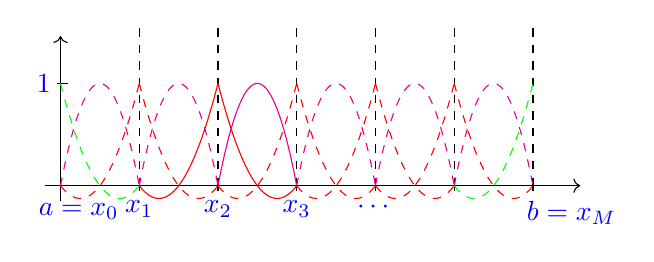
\begin{tikzpicture}
	\draw[->] (-.2,0) -- (6.6,0);
	\draw[->] (0,-.2) -- (0,1.9);		
	
	\draw (-.05,1.3)--(.1,1.3);	
	\foreach \x in {1,2,3,4,5,6}{
		\draw [dashed,thin] (\x,2cm)--(\x,2pt);
		\draw (\x,2pt)--(\x,-2pt);
	}
	\foreach \x/\i in {1/1,2,3/3}
		\node[text=blue,anchor=north] at (\x, -2pt) {$x_\i$};
	
	\node[text=blue,anchor=north] at (4, -2pt) {$\cdots$};
	\node[text=blue,anchor=north west] at (-.4, -3pt) {$a=x_0$};
	\node[text=blue,anchor=north west] at (5.8, -2pt) {$b=x_M$};
	\node[text=blue,anchor=east] at (0,1.3) {1};
	
	\draw[domain=0:1,smooth,variable=\x,xshift=1cm,red] 
		plot ({\x},{1.3*\x*(2*\x-1)});
	\draw[domain=0:1,smooth,variable=\x,xshift=2cm,red] 
		plot ({\x},{1.3*(\x-1)*(2*\x-1)});	
	\draw[domain=0:1,smooth,variable=\x,xshift=2cm,magenta] 
		plot ({\x},{1.3*4*\x*(1-\x)});
	
	\foreach \i/\j in {0/1,2/3,3/4,4/5} {
		\draw[domain=0:1,smooth,variable=\x,xshift=\i cm,red,dashed] 
			plot ({\x},{1.3*\x*(2*\x-1)});	
		\draw[domain=0:1,smooth,variable=\x,xshift=\j cm,red,dashed] 
			plot ({\x},{1.3*(\x-1)*(2*\x-1)});	
		\draw[domain=0:1,smooth,variable=\x,xshift=\j cm,magenta,dashed] 
			plot ({\x},{1.3*4*\x*(1-\x)});
	};		
	\draw[domain=0:1,smooth,variable=\x,xshift=0cm,magenta,dashed] 
		plot ({\x},{1.3*4*\x*(1-\x)});
		
	\draw[domain=0:1,smooth,variable=\x,xshift=0cm,green,dashed] 
		plot ({\x},{1.3*(\x-1)*(2*\x-1)});
	\draw[domain=0:1,smooth,variable=\x,xshift=5cm,green,dashed]
		plot ({\x},{1.3*\x*(2*\x-1)});
\end{tikzpicture}


		\end{minipage}$\longleftarrow$\quad\hfill
		\begin{minipage}{.4\textwidth}
			\vspace{-10pt}
			The interpolation nodes are comprised of the interior nodes
			and midpoints, i.e.
			\[\mathcal{N}:=\mathcal{V}_I(\mathcal{M})\cup\{
				\textrm{midpoints of intervals}\}. \]
		\end{minipage}
	\end{figure}\\
	Here the \textcolor{mid-green}{green} parts are only for the space 
	\[\mathcal{S}_{2}^{0}(\mathcal{M}) := \left\{
		v\in C^0{[a,b]}: v_{|[x_{i-1},x_i]}\ \textrm{quadratic},
		\quad \forall i=1,...,M \right\},\]
	\[ N:=\mathrm{dim}\,\mathcal{S}_{2}^{0}(\mathcal{M})=2M+1.\]
	The space $\mathcal{S}_{2}^{0}(\mathcal{M})$ will be used instead when 
	dealing with non-homogeneous Dirichlet TPBVPs.
	
	We can see that these basis functions satisfy the augmented nodal value
	property ($\cup$ nodal values at midpoints) and they can be split into 
	two categories:
	one corresponds to the interior nodes and the other corresponds to the
	midpoints of those intervals. We denote them by $b_h^i,i=1,...,M-1$ 
	and	$b_h^{i+\frac{1}{2}},i=0,...,M-1$ respectively. For example, in
	the above picture, the red solid graph represents $\textcolor{red}{b_h^2}$
	whose support spans two adjacent intervals and the magenta solid graph 
	represents $\textcolor{magenta}{b_h^{2\frac{1}{2}}}$ whose support only 
	spans one interval.
	
	If we restrict our attention onto one interval, we can extract three local
	shape functions, whose standard versions (reference shape functions, on 
	$[0,1]$) can be rather easily acquired and are shown below. For the sake 
	of comparison we also plot the  reference shape functions of 1st order 
	on its left.	 
	\begin{figure}[!htbp]	
		\centering	
		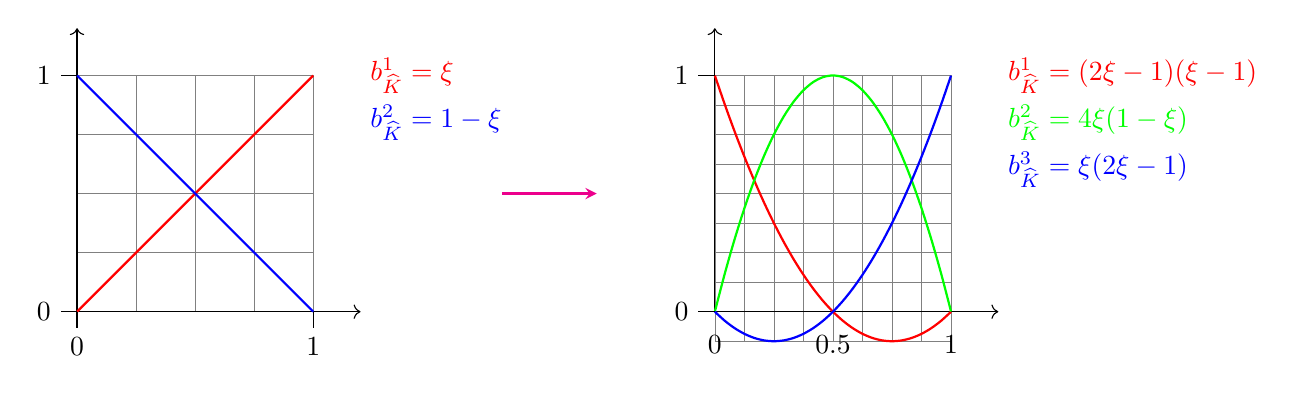
\begin{tikzpicture}[scale=3]
	\draw[step=.25cm,gray,very thin] (0,0) grid (1,1);		
	\draw[->] (0,0) -- (1.2,0);
	\draw[->] (0,0) -- (0,1.2);	
	
	\draw[domain=0:1,smooth,variable=\x,red,thick] 
		plot ({\x},{\x});
	\draw[domain=0:1,smooth,variable=\x,blue,thick] 
		plot ({\x},{1-\x});
	
	\draw (0,0)--(-.07,0) node [anchor=east] {0}
		(0,1)--(-.07,1) node[anchor=east] {1}
		(0,0)--(0,-.07) node [anchor=north] {0}
		(1,0)--(1,-.07) node[anchor=north] {1}
		(1.2,1) node[anchor=west,text=red] {$b_{\widehat{K}}^1=\xi$}
		(1.2,.8) node[anchor=west,text=blue] {$b_{\widehat{K}}^2=1-\xi$};
		
%	====================================================================	
	\draw [>=stealth,->,magenta,thick] (1.8,.5)--(2.2,.5);
%	====================================================================

	\draw[xshift=2.7cm,step=.125cm,gray,very thin] (0,-.125) grid (1,1);		
	\draw[xshift=2.7cm,->] (0,0) -- (1.2,0);
	\draw[xshift=2.7cm,->] (0,0) -- (0,1.2);	

	\draw[xshift=2.7cm,domain=0:1,smooth,variable=\x,red,thick] 
		plot ({\x},{(\x-1)*(2*\x-1)});	
	\draw[xshift=2.7cm,domain=0:1,smooth,variable=\x,green,thick] 
		plot ({\x},{4*\x*(1-\x)});
	\draw[xshift=2.7cm,domain=0:1,smooth,variable=\x,blue,thick] 
		plot ({\x},{\x*(2*\x-1)});
	
	\draw[xshift=2.7cm]
		(0,0)--(-.07,0) node [anchor=east] {0}
		(0,1)--(-.07,1) node[anchor=east] {1}
		(0,-.14) node {0} (.5,-.14) node {0.5} (1.,-.14) node {1}
		(1.2,1) node[anchor=west,text=red]{$b_{\widehat{K}}^1=(2\xi-1)(\xi-1)$}
		(1.2,.8) node[anchor=west,text=green]{$b_{\widehat{K}}^2=4\xi(1-\xi)$}
		(1.2,.6) node[anchor=west,text=blue]{$b_{\widehat{K}}^3=\xi(2\xi-1)$};	
\end{tikzpicture}


	\end{figure}
	
	Since $b_h^i,i=1,...,M-1$ and $b_h^{i+\frac{1}{2}},i=0,...,M-1$
	are the basis functions of the quadratic finite element space 
	$\mathcal{S}_{2,0}^{0}(\mathcal{M})$, then the Galerkin approximation
	$u_h\in U_h:=\mathcal{S}_{2,0}^{0}(\mathcal{M})$ can be uniquely 
	expressed in their linear combinations
	\[u_h=\sum_{i=1}^{M-1}\mu_i b_h^i+
	\sum_{i=0}^{M-1}\mu_{i+\frac{1}{2}} b_h^{i+\frac{1}{2}},\]
	with 
	\[\mu_i=u_h(x_i),\quad \mu_{i+\frac{1}{2}}=u_h(x_{i+\frac{1}{2}}),\]
	that is the basis expansion coefficients are given by the function 
	values of $u_h$ at these interpolation nodes.
	
	The Galerkin matrix now becomes a $(2M-1)$-by-$(2M-1)$	matrix
	with entries
	\[(\bA)_{ij}=a(b_h^j,b_h^i)=\int_{a}^{b}\left(	
	p\frac{\rd b_h^j}{\rd x}\frac{\rd b_h^i}{\rd x}+q b_h^j b_h^i\right)\rd x,
	\quad i,j=\frac{1}{2},1,...,(M-1)\frac{1}{2}.\]
	Of course, the fractional indices may sound a little odd. Therefore in
	practice we	use the transformation 
	\[(i,j)\quad \rightarrow \quad (s,t):=(2i,2j)\]
	to locate the real positions of the entries.
	
	The element matrix is defined on a cell $[x_{i-1},x_i]$ by
	\[\bA_K:=\left[a_K(b_K^j,b_K^l)\right]_{j,l=1}^{3}=\left[
	\int_{x_{i-1}}^{x_i}\left(	
	p\frac{\rd b_K^j}{\rd x}\frac{\rd b_K^l}{\rd x}+q b_K^j b_K^l\right)\rd x
	\right]_{j,l=1}^{3}.\]
	
	Doing the linear transformation $x=x_{i-1}+h_i t,\ h_i:=x_i-x_{i-1}$ 
	we can compute the entries of the element matrix by
	\begin{align*}
		(\bA_K)_{jl}&=\int_{x_{i-1}}^{x_i}\left(	
		p\frac{\rd b_K^j}{\rd x}\frac{\rd b_K^l}{\rd x}+
		q b_K^j b_K^l\right)\rd x\\
		&=\int_{0}^{1} p(x_{i-1}+h_i t)\,
		\frac{\rd\overbrace{b_K^j(x_{i-1}+h_i t)}^{
				=\,\widehat{b}^j(t)}}{h_i\,\rd t}\,
		\rd\overbrace{b_K^l(x_{i-1}+h_i t)}^{=\,\widehat{b}^l(t)}+\\
		&\quad\int_{0}^{1}q(x_{i-1}+h_i t)\,
		\overbrace{b_K^j(x_{i-1}+h_i t)}^{=\,\widehat{b}^j(t)}\,
		\overbrace{b_K^l(x_{i-1}+h_i t)}^{=\,\widehat{b}^l(t)}\, h_i\,\rd t\\
		&=\frac{1}{h_i}\int_{0}^{1} p(x_{i-1}+h_i t)
		\frac{\rd\widehat{b}^j(t)}{\rd t}\frac{\rd\widehat{b}^l(t)}{\rd t}\,
		\rd t+h_i\int_{0}^{1} q(x_{i-1}+h_i t)\,
		\widehat{b}^j(t)\,\widehat{b}^l(t)\,\rd t.
	\end{align*}
	Here $\widehat{b}^j(t):=b_{\widehat{K}}^j(t),\,j=1,2,3$ and hence
	\[\frac{\rd\widehat{b}^1(t)}{\rd t}=4t-3,\qquad
	\frac{\rd\widehat{b}^2(t)}{\rd t}=4-8t,\qquad
	\frac{\rd\widehat{b}^3(t)}{\rd t}=4t-1.\]
	
	The element vector is defined on an interval $[x_{i-1},x_i]$ by
	\[\vv{\bm{\varphi}}_K:=\left[\ell_K(b_K^j)\right]_{j=1}^{3}=
	\left[\int_{x_{j-1}}^{x_i}f(x)b_K^j(x)\,\rd x \right]_{j=1}^{3},\]	
	with entries
	\[(\vv{\bm{\varphi}}_K)_j=
	h_i\int_{0}^{1} f(x_{i-1}+h_i t)\,\widehat{b}^j(t)\,\rd t.\]
	
	Once acquired the element matrices and element vectors we would like to 
	assemble the linear system of equations. This process is illustrated in
	Figure \ref{tikz:1D_assembly_of_quadratic_FE_Galerkin_matrix}. 
	
	We will apply a little trick here. First, it should be noticed that in the 
	1st cell and last cell there are only two local shape functions in them 
	respectively, that is, $b_K^1$ (right half of $b_h^0$) is absent in 
	$[x_0,x_1]$ and $b_K^3$ (left half of $b_h^M$) is absent in $[x_{M-1},x_M]$.
	This means the 1st element matrix should remove all the entries 
	concerning $b_K^1$ which are the 1st row and the 1st column, and the
	last element matrix should get rid of all the entries related to $b_K^3$
	which are the 3rd row and the 3rd column. Next, we consider the assembly
	process in a way that it were in $\mathcal{S}_{2}^{0}(\mathcal{M})$ 
	(pretend each cell has full/3 local shape functions), which will lead to
	a $(2M+1)$-by-$(2M+1)$ Galerkin matrix $\bA$. The assembly is done by
	looping over all cells (loop variable $j=1,...,M-1$) and putting the two 
	adjacent element matrices (corresponding to the cell $[x_{j-1},x_j]$ and
	cell $[x_j,x_{j+1}]$ respectively) together	in a manner such that the 
	$a_{33}$ (lower right) entry of the former element matrix coincides with
	the $a_{11}$ (upper left) entry of the latter element matrix. The value at
	this coinciding position is the sum of these two entries. After the loop
	we just need to extract and reassign the Galerkin matrix: 
	\texttt{A $\gets$ A(2:2M,2:2M)}.
	
	The assembly of the RHS vector is done in the exactly same manner:
	by letting the 3rd entry of the former element vector coincide with
	the 1st entry of the latter element vector and then summing them up.
	Finally, let \texttt{phi $\gets$ phi(2:2M)}.
		
	\begin{figure}[!htbp]	
		\centering
		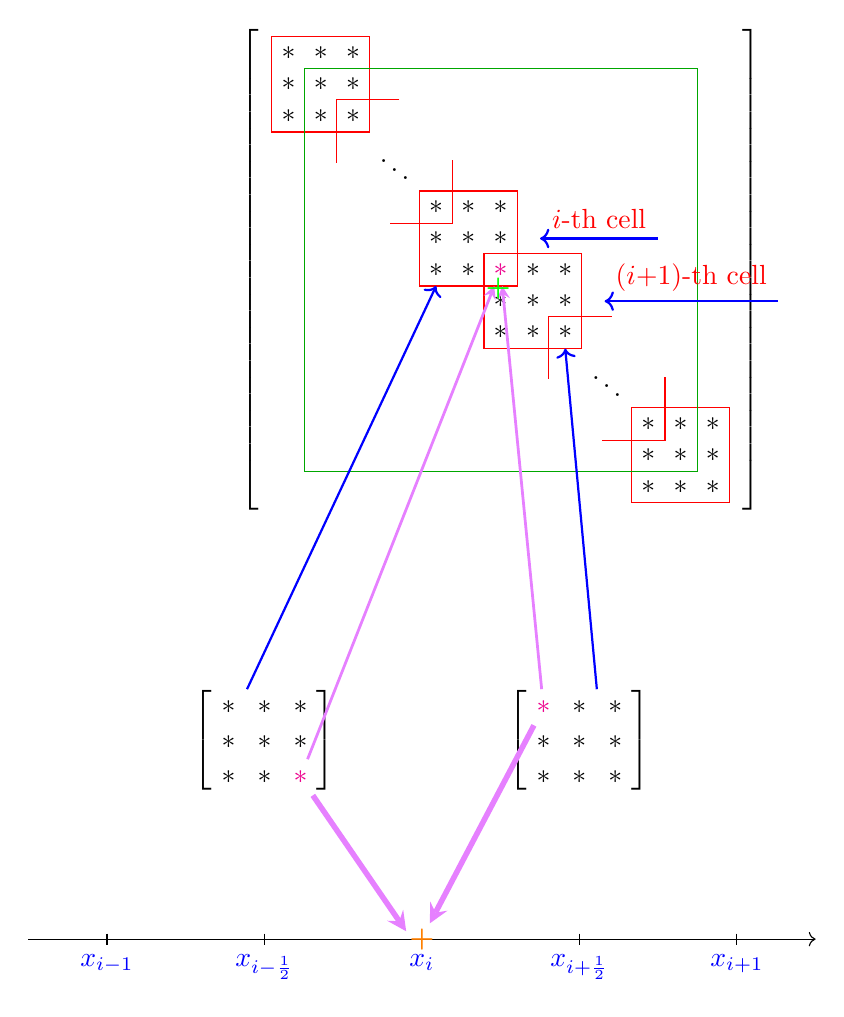
\begin{tikzpicture}
	\draw[->] (0,0) -- (10,0);
	
	\draw 
	(1,2pt)--(1,-2pt) node[anchor=north,text=blue]{$x_{i-1}$}
	(5,2pt)--(5,-2pt) node[anchor=north,text=blue]{$x_{i}$}
	(9,2pt)--(9,-2pt) node[anchor=north,text=blue]{$x_{i+1}$}
	(3,2pt)--(3,-2pt) node[anchor=north,text=blue]{$x_{i-\frac{1}{2}}$}
	(7,2pt)--(7,-2pt) node[anchor=north,text=blue]{$x_{i+\frac{1}{2}}$};
	
	\coordinate (A) at (2,0);
	\coordinate (B) at (5,0);
	\coordinate (C) at (8,0);
	
	\matrix [matrix of math nodes,
	left delimiter={[},
	right delimiter={]},
	inner sep=-2pt,
	nodes={inner sep=.4em},
	row 3 column 3/.style=magenta,
	](M1) at (3,2.5) {
		* &* &*\\
		* &* &*\\
		* &* &*\\ % NOTE that \\ is necessary even for the last row
	};
	\matrix [matrix of math nodes,	
	left delimiter={[},
	right delimiter={]},
	inner sep=-2pt, 
	inner ysep=-2pt,
	nodes={inner sep=.4em},
	row 1 column 1/.style=magenta,
	](M2) at (7,2.5) {
		* &* &*\\
		* &* &*\\
		* &* &*\\
	};
	
	\node[orange] at (B) {$\boldsymbol{+}$};
	\draw[>=stealth,<-,line width=2pt,blue!20!magenta!50]
	(B)+(-.2,.1) -- (M1-3-3);
	\draw[>=stealth,<-,line width=2pt,blue!20!magenta!50]
	(B)+(.1,.2) -- (M2-1-1);
	
%	================================================
	\matrix [matrix of math nodes,	
	left delimiter={[},
	right delimiter={]},
%	inner sep=-2pt, 
%	inner ysep=-2pt,
%	nodes={inner sep=.4em},
	row 7 column 7/.style=magenta,
	](M) at (6,8.5) {% 13-by-13
		* &* &* & & & & & & & & & &\\
		* &* &* & & & & & & & & & &\\
		* &* &* & & & & & & & & & &\\
		& & &\ddots & & & & & & & & & &\\
		& & & &* &* &* & & & & & & &\\
		& & & &* &* &* & & & & & & &\\
		& & & &* &* &* &* &* & & & &\\
		& & & & & &* &* &* & & & &\\
		& & & & & &* &* &* & & & &\\
		& & & & & & & & &\ddots & & &\\
		& & & & & & & & & &* &* &*\\		
		& & & & & & & & & &* &* &*\\
		& & & & & & & & & &* &* &*\\
	};
	\draw[red] (M-1-1.north west) rectangle (M-3-3.south east);
	
	\draw[red] ($(M-3-3.north west)+(0:.8cm)$)--(M-3-3.north west)--
	($(M-3-3.north west)+(-90:.8cm)$);	
	\draw[red] ($(M-5-5.south east)+(90:.8cm)$)--(M-5-5.south east)--
	($(M-5-5.south east)+(180:.8cm)$);
	
	\draw[red] (M-5-5.north west) rectangle (M-7-7.south east);
	\draw[red] (M-7-7.north west) rectangle (M-9-9.south east);
	
	\draw[red] ($(M-9-9.north west)+(0:.8cm)$)--(M-9-9.north west)--
	($(M-9-9.north west)+(-90:.8cm)$);	
	\draw[red] ($(M-11-11.south east)+(90:.8cm)$)--(M-11-11.south east)--
	($(M-11-11.south east)+(180:.8cm)$);
	
	\draw[red] (M-11-11.north west) rectangle (M-13-13.south east);
	
	\draw[mid-green] (M-2-2.north west) rectangle (M-12-12.south east);
	
	\draw[thick,blue,<-] ($(M-6-7.center)+(0:.5cm)$) -- +(0:1.5cm);
	\path ($(M-6-7.center)+(0:1.25cm)$) node[anchor=south,text=red] 
	{$i$-th cell};
	
	\draw[thick,blue,<-] ($(M-8-9.center)+(0:.5cm)$) -- +(0:2.2cm);
	\path ($(M-8-9.center)+(0:1.6cm)$) node[anchor=south,text=red] 
	{$(i\mathtt{+}1)$-th cell};
	
	
%	================================================	
	\draw[->,thick,blue](M1-1-1.north east) -- (M-7-5.south);
	\draw[->,thick,blue](M2-1-3.north west) -- (M-9-9.south);
	
	\draw[>=stealth,->,line width=1pt,blue!20!magenta!50](M1-3-3)--(M-7-7);
	\draw[>=stealth,->,line width=1pt,blue!20!magenta!50](M2-1-1)--(M-7-7);
	
	\node[text=green] at ($(M-7-7)+(-97:7pt)$) {$\boldsymbol{+}$};
	
\end{tikzpicture}


		\caption{Assembly of quadratic FE Galerkin matrix}
		\label{tikz:1D_assembly_of_quadratic_FE_Galerkin_matrix}
	\end{figure}
	
	 
	\vspace{-10pt}
	\section{Numerical Experiments}\label{section.5}
	In this section, we are going to give some numerical examples that use the
	Galerkin finite element method studied in previous sections to solve some
	boundary value problems. A few more examples are provided in Section
	\ref{subsection.6.4} as comparisons to the weak Galerkin (WG) FEM.
	
	\subsection{Example 1}\label{subsection.5.1}
	Our first example is a mixed Neumann-Dirichlet boundary value problem:
	\begin{align*}
		-\Delta{u}=2\pi^2\cos(\pi x)\cos(\pi y),\quad &\textrm{in }\Omega\\
		\nabla{u}\cdot\boldsymbol{n}=\pi\sin(\pi x)\cos(\pi y), 
		\quad&\textrm{on }\Gamma\\
		u=\cos(\pi x)\cos(\pi y),\quad
		&\textrm{on }\partial\Omega\setminus\Gamma,
	\end{align*}
	where $\Omega=\{(x,y)\,|\,-\frac{1}{2} < x < 1,\, -1 < y < 1 \},\ 
	\Gamma = \{(x,y)\,|\, x=-\frac{1}{2},\, -1 \leq y \leq 1 \}$.
	
	Here, the analytic solution is $u=\cos(\pi x)\cos(\pi y)$. We used the 
	Galerkin discretization scheme for linear finite elements developed in 
	Section	\ref{section.2} to solve this BVP. 
	We first give an visual of the solution:
	\begin{figure}[!htbp]
		\makebox[\textwidth][c]{
			{\includegraphics[width=0.45\paperwidth]{svg/LFEM_solution}}
			{\includegraphics[width=0.45\paperwidth]{svg/exact_solution}}
		}
	\end{figure}\vspace{-30pt}

	\begin{figure}[!htbp]
	\begin{minipage}{.5\textwidth}
	One may find that the height of the two graphs seem to disagree. The fact 
	is that the linear FEM solution has some values at some certain points
	exceed 1 which is the maximum value of the analytic solution and is 
	represented in the right-hand side graph. The exceeding values are actually
	very small. The detailed discretization errors in various norms are shown
	in Table \ref{table:example1_convergence_rates} below. By the way, if we
	adopt the general way of computing the right-hand side vector studied in
	Section \ref{subsection.4.2}, i.e. by
	\eqref{eq:2D element vector quadrature formula} as opposed to 
	\eqref{eq:2D element (load) vector formula}, we can indeed gain the same 
	looking of graph as the right-hand side one.
	\end{minipage}%
	\begin{minipage}{.5\textwidth}		
			\includegraphics[width=1\linewidth]{svg/error_estimates}
			\caption{Convergence rates for Example \hyperref[code:example1]{1}}
			\label{fig:error_estimates}		
	\end{minipage}
	\end{figure}

 	The visualization of these results in the table is represented in Figure
 	\ref{fig:error_estimates}.	The MATLAB implementation for Example 1 is 
 	given in Code listing \ref{code:example1}.
	
	\begin{table}[!htbp]
		\caption{Discretization errors and convergence rates in various
			norms for Example \hyperref[code:example1]{1}}\vspace{-5pt}
		\begin{tabular}{rccccccccc}
    \hline
    $N$ & $h_\mathcal{M}:=N^{-\frac{1}{2}}$ & $\norm{e_u}_\infty$ & order & 
    $\norm{e_u}_{L^2(\Omega)}$ & order & $|e_u|_{H^1(\Omega)}$ & order &
    $\norm{e_u}_{H^1(\Omega)}$ & order \Tstrut\Bstrut \\
    \hline
       25    &0.2000    &0.6884    &          &0.4015    &          &2.5890    &          &2.6199    &      \Tstrut\\
       81    &0.1111    &0.1852    &1.8942    &0.1011    &1.9889    &1.3244    &0.9671    &1.3282    &0.9800\\
      289    &0.0588    &0.0474    &1.9646    &0.0254    &1.9931    &0.6663    &0.9911    &0.6668    &0.9942\\
     1089    &0.0303    &0.0119    &1.9904    &0.0064    &1.9979    &0.3337    &0.9976    &0.3338    &0.9984\\
     4225    &0.0154    &0.0030    &1.9975    &0.0016    &1.9994    &0.1669    &0.9994    &0.1669    &0.9996\\
    16641    &0.0078    &0.0007    &1.9994    &0.0004    &1.9999    &0.0835    &0.9998    &0.0835    &0.9999\Bstrut\\
    \hline
\end{tabular}

		\label{table:example1_convergence_rates}
	\end{table}\vspace{-15pt}	
	
	\subsection{Example 2}
	Consider the boundary value problem for Helmholtz equations:
	\begin{align*}
		-\Delta{u} - k^2 u=1,\quad &\textrm{in } G=\,]0,1[\,\times\,]0,1[,\\
		u=0,\quad &\textrm{on }\Gamma_1=\{x=0,0\leq y\leq 1\}\cup
		\{0\leq x \leq 1, y=1\},\\
		\nabla{u}\cdot\boldsymbol{n}=0,\quad &\textrm{on }\Gamma_2=
		\{0\leq x\leq 1,y=0\}\cup\{x=1,0\leq y \leq 1\},
	\end{align*}
	where $k=1,5,10,15,20,25$.
	
	The implementation for Example 2 is given in Code listing
	\ref{code:exercise_2_7_2} and the results are as follows:	
	\begin{figure}[!htbp]
		\makebox[\textwidth][c]{
			{\includegraphics[width=0.45\paperwidth]{svg/Helmholtz_k=1}}
			{\includegraphics[width=0.45\paperwidth]{svg/Helmholtz_k=5}}
		}\\[10pt]
		
		\makebox[\textwidth][c]{
			{\includegraphics[width=0.45\paperwidth]{svg/Helmholtz_k=10}}
			{\includegraphics[width=0.45\paperwidth]{svg/Helmholtz_k=15}}
		}\\[10pt]
		
		\makebox[\textwidth][c]{
			{\includegraphics[width=0.45\paperwidth]{svg/Helmholtz_k=20}}
			{\includegraphics[width=0.45\paperwidth]{svg/Helmholtz_k=25}}
		}
	\end{figure}

	\subsection{Examples for TPBVP}\label{subsection.5.3}
	In this subsection we will have a look at the mixed two-point boundary
	value problem:
	\begin{align*}
		-\frac{\rd}{\rd x}\left(p(x)\frac{\rd u}{\rd x}\right)+q(x)u&=f(x),
		\quad x\in (a,b),\\
		u(a) &= 0,\ u'(b) = 0,
	\end{align*}
	where $p(x) \in C^1(\bar{I}),\; p(x)\geq p_{min}>0,\; 
	q(x) \in  C^1(\bar{I}),\; q(x)\geq 0,\; f(x) \in L^2(I),\;
	I =\,]a,b[ $.
	
	The basis functions of 1st and 2nd order for the above mixed boundary 
	value problem now become something like these:
	\begin{figure}[!htbp]
		\centering
		\begin{minipage}{.5\textwidth}
			\input{input/tikz/1D_tent_functions_mixed_boundary}
		\end{minipage}%
		\begin{minipage}{.5\textwidth}
			\input{input/tikz/1D_quadratic_basis_functions_mixed_BCs}
		\end{minipage}
	\end{figure}
	
	The overall procedures are similar to what we have discussed in
	Section \ref{subsubsection.2.2.1} and Section \ref{subsection.4.5} for
	the 1st order and 2nd order respectively. For example, in the quadratic 
	element version, we just need to let \texttt{A $\gets$ A(2:2M+1,2:2M+1)}.
	
	We will consider two test cases both of which set $p(x)=1,\,q(x)=0,\,
	[a,b]=[0,3]$.
	
	Test case 1:
	\[ f= \frac{\pi^2}{4} \sin(\frac{\pi}{2}x),\quad 
	\textrm{with } u=\sin(\frac{\pi}{2}x).
	\]
	
	Test case 2:
	\[ f = \pi^2\sin(\pi x),\quad 
	\textrm{with } u=\sin(\pi x)+\pi x.
	\]
	
	The approximations are given in Figure \ref{fig:1D L/Q FEM approximations}
	and the graphs concerning the convergence rates of 1st order and 2nd order
	for Test case 1 are represented in Figure 
	\ref{fig:1D convergence rates for test case 1}.
	
	We can conclude from Figure \ref{fig:1D convergence rates for test case 1}
	that the convergence rates for \emph{linear} finite elements are
	\[L^\infty \textrm{ norm}:\, O(h^2),\qquad L^2 \textrm{ norm}:\, O(h^2),
	\qquad H^1 \textrm{ norm}:\, O(h),\]	
	and for \emph{quadratic} finite elements are
	\[L^\infty \textrm{ norm}:\, O(h^3),\qquad L^2 \textrm{ norm}:\, O(h^3),
	\qquad H^1 \textrm{ norm}:\, O(h^2).\]
	
	These results agree with the theory, that is for $p$-th order finite 
	elements:
	\[L^\infty \textrm{ norm}:\, O(h^{p+1}),\qquad L^2 \textrm{ norm}:\, 
	O(h^{p+1}),	\qquad H^1 \textrm{ norm}:\, O(h^p).\]
		
%	\clearpage
	\begin{figure}[!htbp]
		\makebox[\textwidth][c]{			
			\subfloat[Test case 1 by LFEM]
			{\includegraphics[width=0.45\paperwidth]
				{svg/FEM1d/problem1}}
			\subfloat[Test case 1 by QFEM]
			{\includegraphics[width=0.45\paperwidth]
				{svg/FEM1d/problem1_quad}}
		}\\
		\makebox[\textwidth][c]{
			\subfloat[Test case 2 by LFEM]
			{\includegraphics[width=0.45\paperwidth]
				{svg/FEM1d/problem2}}
			\subfloat[Test case 2 by QFEM]
			{\includegraphics[width=0.45\paperwidth]
				{svg/FEM1d/problem2_quad}}
		}	
		\caption{Approximations via Linear FEM \& Quadratic FEM}
		\label{fig:1D L/Q FEM approximations}
	\end{figure}
	
	\begin{figure}[!htbp]
		\makebox[\textwidth][c]{
			\subfloat[Convergence in $L^\infty$ norm]
			{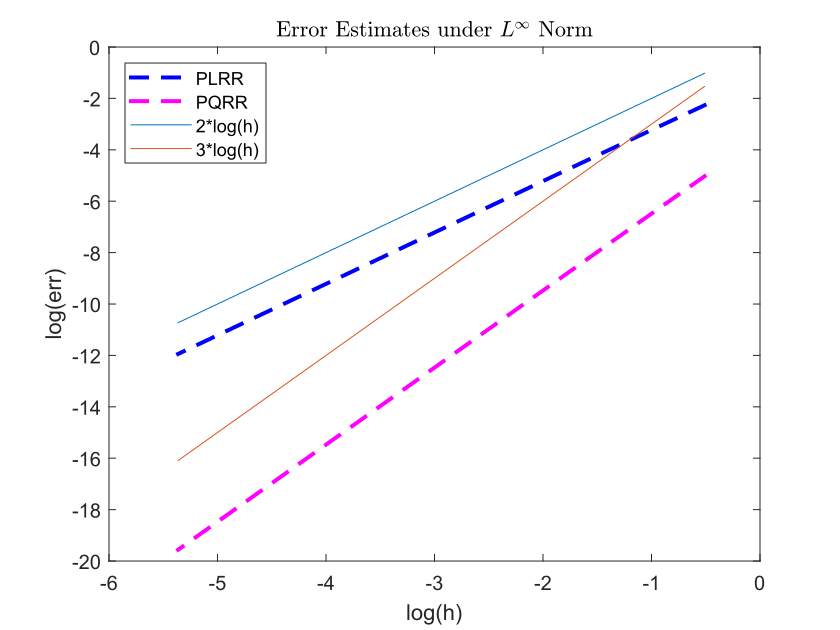
\includegraphics[width=0.31\paperwidth]{svg/FEM1d/L_inf_norm}}
			\subfloat[Convergence in $L^2$ norm]
			{\includegraphics[width=0.31\paperwidth]{svg/FEM1d/L2_norm}}
			\subfloat[Convergence in $H^1$ norm]
			{\includegraphics[width=0.31\paperwidth]{svg/FEM1d/H1_norm}}
		}
		\caption{Convergence rates for Test case 1}
		\label{fig:1D convergence rates for test case 1}
	\end{figure}
	
	\clearpage
	\section{Further Reading---A Weak Galerkin FEM}\label{section.6}
	\fancyhead[L]{6\quad A WEAK GALERKIN FEM}		
	In the end, as a further reading, we introduce a more advanced
	technique---the weak Galerkin method. It was first introduced and analyzed
	by Junping Wang and Xiu Ye in their paper \cite{WG2013} for solving
	second-order elliptic problems. The weak Galerkin 
%	is a finite element method that uses a weakly defined gradient 
%	operator over generalized functions.
	is an original finite element method based on variational principles for 
	weak (generalized) functions and the weak gradients defined thereon.
	
	To illustrate the main ideas of weak Galerkin, the model problem we	will 
	consider here is the Dirichlet problem for 2nd-order elliptic equations
	\begin{align}
		-\nabla\cdot(\mathcal{A}\nabla u)=f,\quad &\textrm{in }\Omega,
		\label{eq:WG PDE}\\
		u=g,\quad &\textrm{on }\partial\Omega,\label{eq:WG Dir BC}
	\end{align}
	where $\Omega$ is an open bounded domain in $\mathbb{R}^d$ (polygonal for
	$d=2$, polyhedral for $d=3$) and $\mathcal{A}$ is a symmetric uniformly 
	positive definite $d\times d$ matrix-valued function.

	\subsection{Weak Gradients and Discrete Weak Gradients}
	As the weak Galerkin draws its strength from introducing the weak gradient
	operator, we shall first elaborate on the definitions.
	
	Let $T$ be any polytopal domain with boundary $\partial T$. A weak function
	on the region $T$ refers to a function $v=\{v_0,v_b\}$ satisfying 
	$v_0\in L^2(T)$ and $v_b\in L^2(\partial T)$. One can interpret the 1st
	component $v_0$ as the value of $v\in T$, and the 2nd component $v_b$
	as the value of $v$ on $\partial T$. We point out that $v_b$ may
	not necessarily be associated with the trace of $v_0$ on $\partial T$. We 
	denote the space of weak functions on $T$ by $W(T)$, that is,
	\[ W(T)=\{v=\{v_0,v_b\}:\, v_0 \in L^2(T),\, v_b\in L^2(\partial T)\}.\]	
	For ease of writing, we use the notations 
	$(v,w)_D\,\hat{=}\,\int_D vw\,\dx$ with $D\in\mathbb{R}^d$ and
	$\inangle{v,w}_\gamma\,\hat{=}\,\int_\gamma vw\,\rd s$ with
	$\gamma\in\mathbb{R}^{d-1}$.
	
	\begin{definition}
	$\forall v\in W(T)$, we define the weak gradient of $v$ as a linear 
	functional $\nabla_w v$	in the dual space of $H^1(T)$ whose action on each
	$q\in[H^1(T)]^d$ is given by 
	\begin{equation}\label{def:weak gradient}
		\inangle{\nabla_w v,q}_T := - (v_0, \nabla\cdot q)_T+
		\inangle{v_b, q\cdot\bm{n}}_{\partial T}.
	\end{equation}
	Here, $\bm{n}$ is the outward normal direction to $\partial T$.
	\end{definition}

	Note that for any $v\in W(T)$, the right-hand side of 
	\eqref{def:weak gradient} defines a bounded linear functional on the 
	normed linear space $H^1(T)$. Therefore, the weak gradient $\nabla_w v$ 
	is well defined. In addition, if the component of $v$ are restrictions of
	a function $u\in H^1(T)$ in $T$ and on $\partial T$, respectively, then
	we arrive at
	\[-(v_0,\nabla\cdot q)_T + \inangle{v_b, q\cdot\bm{n}}_{\partial T}=
	-(u,\nabla\cdot q)_T + \inangle{u, q\cdot\bm{n}}_{\partial T}=
	-(\nabla u\cdot q, 1)_T,\]
	which suggests $\nabla_w v=\nabla u$, i.e. the strong gradient of 
	$u$.
	
	In another view, we can the embed Sobolev space $H^1(T)$ into the space 
	$W(T)$ through an inclusion map: $H^1(T)\mapsto W(T)$ which is defined by
	\[ i_w(\phi) = \{\phi|_T,\phi|_{\partial T}\},\quad \phi\in H^1(T).\]	
	Aided by the inclusion map $i_w$, one can view the Sobolev space $H^1(T)$ 
	as a subspace of $W(T)$ via distinguishing each $\phi\in H^1(T)$ with 
	$i_w(\phi)$. Similarly, a weak function $v=\{v_0,v_b\}\in W(T)$ is said
	to be in $H^1(T)$ if it can be recognized by a function $\phi\in H^1(T)$
	through $i_w(\phi)$. This, again, suggests that 
	the weak gradient amounts to the classical gradient 
	(that is, $\nabla_w v=\nabla u$) for smooth functions $v\in H^1(T)$. 
	
	The discrete weak gradient operator is introduced
	in the sense such that $\nabla_w$ is approximated in a polynomial subspace 
	of the dual $[H^1(T)]^d$. We will 
	adopt the notation $[P_r(T)]^d$ to mean the set of polynomials on $T$ with 
	degree $\leq r$.
	
	\begin{definition}
	The discrete weak gradient operator, denoted by $\nabla_{w,r,T}$, is defined
	as the unique polynomial $(\nabla_{w,r,T}v)\in[P_r(T)]^d$ that meets 
	\begin{equation}\label{def:discrete weak gradient}
		(\nabla_{w,r,T}v,q)_T := -(v_0,\nabla\cdot q)+
		\inangle{v_b,q\cdot\bm{n}}_{\partial T}, \quad q\in[P_r(T)]^d.
	\end{equation}
	\end{definition}
	Using integration by parts to the first term on the right-hand side of
	\eqref{def:discrete weak gradient}, one can rephrase
	\eqref{def:discrete weak gradient} in the following form
	\begin{equation}\label{eq:rewrite of dwg}
		(\nabla_{w,r,T}v,q)=(\nabla v_0,q)_T+
		\inangle{v_b-v_0,q\cdot\bm{n}}_{\partial T}, \quad q\in[P_r(T)]^d.		
	\end{equation}

	\begin{remark}
	We point out that in the design	of numerical methods for partial 
	differential equations, the classical 
	gradient operator $\nabla=(\partial_{x_1},\partial_{x_2})$ should be 
	employed to functions with some certain degree of smoothness.
	For instance, in the standard Galerkin FEM, continuous piecewise 
	polynomials over a prescribed finite element partition is often implied on 
	such a ``smoothness". By introducing the weak gradient operator, 
	derivatives can be taken for functions \emph{without 
	any	continuity} across cells on a mesh (amazing). In this way, the 
	notion of weak gradient \emph{permits the use of generalized functions}
	in approximation.
	\end{remark}

	\subsection{Weak Galerkin Finite Element Schemes}
	Denote by $\mathcal{T}_h$ a partition of the domain $\Omega$ comprising 
	polygons in 2D or polyhedrons in 3D qualified with a set of rules as 
	specified in \cite{WGmixed2014}. We denote the set of all 
	edges or flat faces in $\mathcal{T}_h$ by $\mathcal{E}_h$.
	The set of all interior edges or faces is represented by 
	$\mathcal{E}_h^0=\mathcal{E}_h\setminus\partial\Omega$.
	$\forall T\in\mathcal{T}_h$, its diameter
	is denoted by $h_T$, and the mesh size is denoted by
	$h=\max_{T\in\mathcal{T}_h} h_T$ for $\mathcal{T}_h$.
	We assume the mesh is quasi-uniform, that is to say there exists a 
	constant satisfying $h\leq Ch_T,\,\forall T\in\mathcal{T}_h$.
	
	For a given integer $k\geq 1$, denote by $V_h$ the weak Galerkin finite 
	element space concerning $T_h$ defined by
	\begin{equation}
		V_h=\{v=\{v0_,v_b\}:\,v_0|_T\in P_k(T),\,v_b|e\in P_{k-1}(e),\,
		e\subset\partial T,\,T\in\mathcal{T}_h \}
	\end{equation}
	and
	\begin{equation}
		V_h^0=\{v:\,v\in V_h,\, v_b=0 \textrm{ on } \partial\Omega\}.
	\end{equation}
	It should be emphasized that for any function $v\in V_h$ there exists a 
	single value $v_b$ on each edge $e\in\mathcal{E}_h$.
	
	For every element $T\in\mathcal{T}_h$, we denote the $L^2$ projection
	from $L^2(T)$ to $P_k(T)$ by $Q_0$ and denote the $L^2$ projection from 
	$L^2(e)$ to $P_{k-1}(e)$ by $Q_b$. Denote by $\mathbb{Q}_h$ the $L^2$ 
	projection from $[L^2(T)]^d$ to the discrete gradient space 
	$[P_{k-1}(T)]^d$. 
	Let $V=H^1(\Omega)$. A projection operator is defined by $Q_h:V\mapsto V_h$ 
	satisfying
	\begin{equation}
		Q_h v=\{Q_0 v_0, Q_b v_b\}, \quad \{v_0,v_b\}=i_w(v)\in W(T),
		\quad T\in\mathcal{T}_h
	\end{equation}
	We denote the discrete weak gradient operator on the 
	finite element space $V_h$ by $\nabla_w,{k-1}$, then we can compute it by 
	using \eqref{def:discrete weak gradient} on each element $T$, that is
	\[ (\nabla_{w,k-1}v)|_T=\nabla_{w,k-1,T}(v|_T),\quad v\in V_h.\]
	We will drop the subscript $k-1$
	in $\nabla_{w,k-1}$ for the discrete weak gradient from now on for the sake 
	of simplicity.
	
	Consider two forms on $V_h$:
	\[a(v,w)=\sum_{T\in\mathcal{T}_h} (a\nabla_w v,\nabla_w w)_T,\]
	\[s(v,w)=\rho \sum_{T\in\mathcal{T}_h}h_T^{-1}
	\inangle{Q_b v_0-v_b,Q_b w_0-w_b}_{\partial T},\]
	where $\rho>0$. We will take $\rho=1$
	throughout this section for the sake of simplicity. We denote a 
	stabilization $a_s(\cdot,\cdot)$ of $a(\cdot,\cdot)$ with
	\[a_s(v,w)=a(v,w)+s(v,w).\]
	
	\textbf{Weak Galerkin Algorithm 1.} We are assigned to find 
	$u_h=\{u_0,u_b\}\in V_h$ such that
	$u_b=Q_b g$ on $\partial\Omega$ and satisfying:
	\begin{equation}\label{eq:WG scheme}
		a_s(u_h,v)=(f,v_0),\quad \forall v=\{v_0,v_b\}\in V_h^0.
	\end{equation}

	To justify the well-posedness of the scheme \eqref{eq:WG scheme}, we let
	\begin{equation}
		\vertiii{v}:=\sqrt{a_s(v,v)}\quad \forall v\in V_h .
	\end{equation}
	A semi-norm in $V_h$ is defined by the functional $\vertiii{\cdot}$. 
	Moreover, a norm in $V_h^0$ is also defined. To confirm this, all we
	need to do is check the	positivity property for $\vertiii{\cdot}$. In the 
	end, we suppose
	$v\in V_h^0$ and $\vertiii{v}=0$. It follows that
	\[(a\nabla_w v,\nabla_w v)+\sum_{T\in\mathcal{T}_h} h_T^{-1}
		\inangle{Q_b v_0-v_b,Q_b v_0-v_b}_{\partial T}=0,\]
	which suggests that $\nabla_w v=0$ for every element $T$ and $Q_b v_0=v_b$
	on $\partial T$. Then by $\nabla_w v=0$ and 
	\eqref{eq:rewrite of dwg} we have $\forall q\in [P_{k-1}(T)]^d$
	\begin{align*}
		0&=(\nabla_w v,q)_T\\
		&=(\nabla v_0,q)_T - \inangle{v_0-v_b,q\cdot\bm{n}}_{\partial T}\\
		&=(\nabla v_0,q)_T-\inangle{Q_b v_0-v_b,q\cdot\bm{n}}_{\partial T}\\
		&=(\nabla v_0,q)_T.	
	\end{align*}
	By letting $q=\nabla v_0$ in the above equation gives $\nabla v_0=0$ on 
	$T\in\mathcal{T}_h$. Therefore, $v_0=const\quad\forall T\in\mathcal{T}_h$.
	This, alone with the fact that $Q_b v_0=v_b$ on $\partial T$ and 
	$v_b=0$ on $\partial\Omega$, suggests $v_0=v_b=0$.
	
	\begin{lemma}
		The weak Galerkin finite element scheme \eqref{eq:WG scheme}
		has one and only one solution.
	\end{lemma}
	\begin{proof}
	Obviously, we just need to shown the uniqueness. Let $u_h^{(1)}$ and 
	$u_h^{(2)}$ be two
	solutions of \eqref{eq:WG scheme}, it follows that  
	$e_h=u_h^{(1)}-u_h^{(2)}$ satisfies
	\[a_s(e_h,v)=0, \quad \forall v\in V_h^0.\]
	Note that $e_h\in V_h^0$, then substituting $v$ with $e_h$ in the above 
	equation gives
	\[ \vertiii{e_h}^2=a_s(e_h,e_h)=0.\]
	This suggests $e_h\equiv0$, or equivalently, $u_h^{(1)}\equiv u_h^{(1)}$. 
	This yields the assertion of the lemma.
	\end{proof}
	
	\subsection{Error Analysis for Weak Galerkin}	
	The overall error analysis for the weak Galerkin is rather complicated,
	so we will simply give some conclusions. For more information about the 
	proofs, one can refer to \cite[Section 5, 6]{WG2015}.
	
	\subsubsection*{Error Equation}
	\bookmark[dest=\HyperLocalCurrentHref, level=3]{Error Equation}
	Let $u_h=\{u_o,u_b\}\in V_h$ be the weak Galerkin finite element solution
	arising from the numerical scheme \eqref{eq:WG scheme}. Assume $u$ the exact
	solution of (\ref{eq:WG PDE},~\ref{eq:WG Dir BC}). The
	$L^2$ projection of $u$ in the finite element space $V_h$ is given by
	\[Q_h u=\{Q_0 u,Q_b u\}.\]
	Let
	\[e_h=\{e_0,e_b\}=\{Q_0 u-u_0,Q_b u-u_b\}\]
	be the error between the WG finite element solution and the $L^2$
	projection of the exact solution.
	
	\begin{lemma}
	Let $e_h$ be the error of the weak Galerkin finite element solution 
	arising from \eqref{eq:WG scheme}. Then we have
	\begin{equation}\label{eq:WG eq6.1}
		a_s(e_h,v)=\ell_u(v)+s(Q_h u,v), \quad \forall v\in V_h^0,
	\end{equation}
	where $\ell_u(v) = \sum_{T\in\mathcal{T}_h}\inangle{a(\nabla u-
		\mathbb{Q}_h\nabla u)\cdot\bm{n},v_0-v_b}_{\partial T}$.	
	\end{lemma}	
	
	\subsubsection*{Error Estimates}
	\bookmark[dest=\HyperLocalCurrentHref, level=3]{Error Estimates}	
	\begin{theorem}
	Let $u_h\in V_h$ be the weak Galerkin finite element solution of the
	model problem (\ref{eq:WG PDE},~\ref{eq:WG Dir BC}) arising from
	\eqref{eq:WG scheme}. Assume the exact solution $u\in H^{k+1}(\Omega)$.
	Then, there exists a constant $C$ such that
	\begin{equation}\label{eq:WG eq6.5}
		\vertiii{u_h-Q_h u}\leq Ch^K \norm{u}_{k+1}.
	\end{equation}	
	\end{theorem}
	
	\begin{corollary}
	Let $u_h\in V_h$ be the weak Galerkin finite element solution of the model
	problem (\ref{eq:WG PDE},~\ref{eq:WG Dir BC}) arising from 
	\eqref{eq:WG scheme}. Assume the exact solution $u\in H^{k+1}(\Omega)$.
	Then, there exists a constant $C$ such that 
	\begin{equation}
		\norm{u-u_h}_{1,h}\leq Ch^k\norm{u}_{k+1}.		
	\end{equation}
	\end{corollary}
	
	Consider the dual problem 
	\begin{equation}\label{eq:WG eq6.8}
		\begin{cases}
			\textrm{Find }\Phi\in H_1^0(\Omega) \textrm{ such that}\\
			-\nabla\cdot(a\nabla\Phi)=e_0 \quad \textrm{in } \Omega.
		\end{cases}
	\end{equation}
	The usual $H^2$-regularity is assumed, which
	means there  exists a Constant $C$ such that
	\begin{equation}
		\norm{\Phi}_2 \leq C\norm{e_0}.
	\end{equation}
	
	\begin{theorem}
	Let $u_h\in V_h$ be the weak Galerkin finite element solution of problem
	(\ref{eq:WG PDE},~\ref{eq:WG Dir BC}) arising from $\eqref{eq:WG scheme}$.
	Assume the exact solution $u\in H^{k+1}(\Omega)$. Moreover, assume the
	dual problem \eqref{eq:WG eq6.8} has the usual $H^2$-regularity. Then,
	there exists a constant $C$ such that
	\begin{equation}
		\norm{u-u_0}\leq Ch^{k+1}\norm{u}_{k+1}.
	\end{equation}
	\end{theorem}

	\subsection{Comparison to Standard FEM}\label{subsection.6.4}
	In this subsection, we will check out differences of the  quality 
	of approximation between the weak Galerkin finite element method and the 
	standard Galerkin FEM developed in previous sections by a few numerical
	experiments. For simplicity, the domain is set with
	$\Omega=\,]0,1[ \times ]0,1[$ for \emph{all} the comparison examples below, 
	and	in the rest of this subsection we will just call these two methods WG 
	and	SG.	The MATLAB implementation for all these comparison examples by 
	SG is given in Code listing \ref{code:ellbvp_Dir}.
	
	For the weak Galerkin, the error is defined by $e_h=u_h-Q_h u=\{e_0,e_b\}$,
	where $e_0=u_0-Q_0 u$ and $e_b=u_b-Q_b u$. Here $Q_hu=\{Q_0 u, Q_b u\}$
	with $Q_h$ as the $L^2$ projection onto approximately defined spaces.
	
	\subsubsection*{Comparison Example 1}
	\bookmark[dest=\HyperLocalCurrentHref, level=3]{Comparison Example 1}
	The first comparison example is set with
	\[\mathcal{A}=\begin{bmatrix}
		x^2+y^2+1 & xy \\
		xy	& x^2+y^2+1
	\end{bmatrix},\quad \textrm{with } u=\sin(\pi x)\cos(\pi y).\]
	To match the equations, the Dirichlet boundary function $g$ and source 
	function $f$ are thus set to be
	\[\begin{split}
		f=&-\pi[ 3x\cos(\pi x)\cos(\pi y)-2\pi xy\cos(\pi x)\sin(\pi y)-\\
		&2\pi(x^2+y^2+1)\sin(\pi x)\cos(\pi y)-3y\sin(\pi x)\sin(\pi y) ], 
	\end{split}\]
	and 
	\begin{equation}\label{eq:Comp Ex1 g}
		g=\begin{cases}
			0,&\quad x=0\ \textrm{or }1,\ 0\leq y \leq 1,\\
			sin(\pi x) &\quad y=0,\ 0\leq x \leq 1,\\
			-sin(\pi x) &\quad y=1,\ 0\leq x \leq 1,
		\end{cases}.
	\end{equation}

	The corresponding numerical results by WG and SG are shown in 
	Table \ref{table:WG_u1a_convergence_rates} and 
	Table \ref{table:SG_u1a_convergence_rates}, respectively.
	
		
	\begin{table}[!htbp]
	\begin{mdframed}[linecolor=red,linewidth=.5pt,roundcorner=10pt]
		\centering
		\caption{Comparison example 1 by WG}\vspace{-5pt}
		\begin{tabular}{lllll}
    \hline
    $h$ & $\vertiii{e_h}$ & Order & $\norm{e_0}$ & Order \Tstrut\Bstrut \\
    \hline    
    1/4      &1.3240e\Plus00     &                &1.5784e\Plus00             \Tstrut\\
    1/8      &6.6333e\Minus01     &9.9710e-01     &3.6890e\Minus01     &2.0972\\
    1/16     &3.3182e\Minus01     &9.9933e-01     &9.0622e\Minus02     &2.0253\\
    1/32     &1.6593e\Minus01     &9.9983e-01     &2.2556e\Minus02     &2.0064\\
    1/64     &8.2966e\Minus02     &9.9998e-01     &5.6326e\Minus03     &2.0016\\ 
    1/128    &4.1483e\Minus02     &1.0000         &1.4078e\Minus03     &2.0004\Bstrut\\
    \hline
\end{tabular}

		\label{table:WG_u1a_convergence_rates}
		\vspace{10pt}
		\caption{Comparison example 1 by standard FEM}\vspace{-5pt}
		\begin{tabular}{lcccccccc}
    \hline
    $h_\mathcal{M}:=n^{-1}$ & $\norm{e_u}_\infty$ & order & 
    $\norm{e_u}_{L^2(\Omega)}$ & order & $|e_u|_{H^1(\Omega)}$ & order &
    $\norm{e_u}_{H^1(\Omega)}$ & order \Tstrut\Bstrut \\
    \hline
      1/4    &0.0293    &          &0.0644    &          &0.8442    &          &0.8466    &      \Tstrut\\
      1/8    &0.0081    &1.8620    &0.0176    &1.8739    &0.4325    &0.9648    &0.4329    &0.9678\\
     1/16    &0.0021    &1.9284    &0.0045    &1.9657    &0.2176    &0.9908    &0.2177    &0.9917\\
     1/32    &0.0005    &1.9868    &0.0011    &1.9912    &0.1090    &0.9977    &0.1090    &0.9979\\
     1/64    &0.0001    &1.9978    &0.0003    &1.9978    &0.0545    &0.9994    &0.0545    &0.9995\\
    1/128    &0.0000    &1.9989    &0.0001    &1.9994    &0.0273    &0.9999    &0.0273    &0.9999\Bstrut\\ \hline\Tstrut
$O(h^r),r=$  &          &1.9599    &          &1.9713    &          &0.9921    &          &0.9928\Bstrut\\
    \hline
\end{tabular}

		\label{table:SG_u1a_convergence_rates}
	\end{mdframed}
	\end{table}\vspace{-5pt}
	
	\subsubsection*{Comparison Example 2}
	\bookmark[dest=\HyperLocalCurrentHref, level=3]{Comparison Example 2}
	The Poisson problem is considered in our second example:
	\[-\Delta u=f\]
	for the PDE model as in \eqref{eq:WG PDE}. Still, we use the exact solution
	$u=\sin(\pi x)\cos(\pi y)$ as the first example did. Hence the source 
	function $f$ becomes
	\[ f=2\pi^2\sin(\pi x)\cos(\pi y) \]
	and boundary function $g$ is given by \eqref{eq:Comp Ex1 g} as before.
	
	The results for Comp Ex 2 by WG and SG are shown in 
	Table \ref{table:WG_u1b_convergence_rates} and 
	Table \ref{table:SG_u1b_convergence_rates}, respectively.

	\begin{table}[!htbp]
	\begin{mdframed}[linecolor=red,linewidth=.5pt,roundcorner=10pt]
		\centering
		\caption{Comparison example 2 by WG}\vspace{-5pt}
		\begin{tabular}{llll}
    \hline
    $h$ & $\vertiii{e_h}$ & $\norm{e_h}$ & $\norm{e_h}_{\mathcal{E}_h}$ \Tstrut\Bstrut \\
    \hline
    1/2      &2.7935e\Minus01      &6.1268e\Minus01      &5.7099e\Minus02\Tstrut\\                
    1/4      &1.4354e\Minus01      &1.5876e\Minus01      &1.3892e\Minus02\\
    1/8      &7.2436e\Minus02      &4.0043e\Minus02      &3.5430e\Minus03\\
    1/16     &3.6315e\Minus02      &1.0033e\Minus02      &8.9325e\Minus04\\
    1/32     &1.8170e\Minus02      &2.5095e\Minus03      &2.2384e\Minus04\\
    1/64     &9.0865e\Minus03      &6.2747e\Minus04      &5.5994e\Minus05\\
    1/128    &4.5435e\Minus03      &1.5687e\Minus04      &1.4001e\Minus05\\
    1/256    &2.2718e\Minus03      &3.9219e\Minus05      &3.5003e\Minus06\Bstrut\\
$O(h^r),r=$  &9.9388e\Minus01      &1.9931               &1.9961\Bstrut\\ 
    \hline
\end{tabular}

		\label{table:WG_u1b_convergence_rates}
		\vspace{10pt}
		\caption{Comparison example 2 by SG}\vspace{-5pt}
		\begin{tabular}{lcccccccc}
    \hline
    $h_\mathcal{M}:=n^{-1}$ & $\norm{e_u}_\infty$ & order & 
    $\norm{e_u}_{L^2(\Omega)}$ & order & $|e_u|_{H^1(\Omega)}$ & order &
    $\norm{e_u}_{H^1(\Omega)}$ & order \Tstrut\Bstrut \\
    \hline
      1/4    &0.0223    &          &0.0636    &          &0.8440    &          &0.8464    &      \Tstrut\\
      1/8    &0.0059    &1.9235    &0.0172    &1.8863    &0.4325    &0.9646    &0.4328    &0.9676\\
     1/16    &0.0015    &1.9525    &0.0044    &1.9699    &0.2176    &0.9908    &0.2177    &0.9916\\
     1/32    &0.0004    &1.9752    &0.0011    &1.9924    &0.1090    &0.9977    &0.1090    &0.9979\\
     1/64    &0.0001    &1.9988    &0.0003    &1.9981    &0.0545    &0.9994    &0.0545    &0.9995\\
    1/128    &0.0000    &1.9992    &0.0001    &1.9995    &0.0273    &0.9999    &0.0273    &0.9999\Bstrut\\ \hline\Tstrut
$O(h^r),r=$  &          &1.9714    &          &1.9744    &          &0.9921    &          &0.9928\Bstrut\\ 
    \hline
\end{tabular}

		\label{table:SG_u1b_convergence_rates}
	\end{mdframed}
	\end{table}

	The next two comparison examples are taken from the paper \cite{WG2012}.
%	We will first give some definitions here, which will be used later in
%	the numerical results.
	
	\subsubsection*{Comparison Example 3}
	\bookmark[dest=\HyperLocalCurrentHref, level=3]{Comparison Example 3}
	The 3rd comparison example we use here is a degenerated diffusion problem.
	
	Consider
	\begin{align*}
		-\nabla \cdot(xy\nabla u)=f,\quad &\textrm{in } \Omega\\
		u=0. \quad &\textrm{on } \partial\Omega
	\end{align*}
	The exact solution is set to be $u=x(1-x)y(1-y)$ given that it vanishes on 
	the boundary.

	The interesting thing is the diffusion tensor $\mathcal{A}=xy$ is not
	uniformly positive definite (see the 2nd footnote on page 2), that is,
	we can't find such a positive number $\epsilon^- >0$ such that
	\[ ((xy) \bm(z))\cdot \bm{z} \geq \epsilon^- \norm{\bm{z}}^2 
		\quad \forall\bm{z}\in\mathbb{R}^2\]
	holds for almost all $(x,y)\in\Omega=\,]0,1[\times]0,1]$.
	Hence, the convergence rates in these norms by which we have usually 
	measured are not specified. This applies both to WG and SG. So we cannot 
	expect the orders of the convergent rates.
	
	These numerical results are given in Table 
	\ref{table:WG_u2_convergence_rates}	and Table 
	\ref{table:SG_u2_convergence_rates} for WG and SG, respectively. 
	
		

	\begin{table}[!htbp]
	\begin{mdframed}[linecolor=red,linewidth=.5pt,roundcorner=10pt]
		\centering
		\caption{Comparison example 3 by WG}\vspace{-5pt}
		\begin{tabular}{lcccccc}
    \hline
    $h$ & $\norm{\nabla_d e_h}$ & $\norm{e_0}$ & $\norm{e_b}$ & $\norm{\nabla_d u_h \nabla u}$ 
    & $\norm{u_0-u}$ & $\norm{e_0}_\infty$ \Tstrut\Bstrut \\
    \hline
    1/8     &5.61e\Minus02    &3.32e\Minus03    &6.60e\Minus03    &5.75e\Minus02    &5.48e\Minus03   &1.27e\Minus02\Tstrut\\
    1/16    &4.03e\Minus02    &1.38e\Minus03    &2.81e\Minus03    &4.09e\Minus02    &2.59e\Minus03   &4.90e\Minus03\\
    1/32    &2.95e\Minus02    &5.68e\Minus04    &1.16e\Minus03    &2.96e\Minus02    &1.23e\Minus03   &2.21e\Minus03\\
    1/64    &2.15e\Minus02    &2.35e\Minus04    &4.83e\Minus04    &2.15e\Minus02    &5.97e\Minus04   &1.16e\Minus03\\
    1/128   &1.55e\Minus02    &9.93e\Minus05    &2.02e\Minus04    &1.55e\Minus02    &2.91e\Minus04   &5.99e\Minus04\Bstrut\\
    \hline\Tstrut
$O(h^r),r=$ &0.4614           &1.2687           &1.2594           &0.4697           &1.0579          &1.0912\Bstrut\\ 
    \hline
\end{tabular}

		\label{table:WG_u2_convergence_rates}
		\vspace{10pt}
		\caption{Comparison example 3 by SG}\vspace{-5pt}
		\begin{tabular}{lcccccccc}
    \hline
    $h_\mathcal{M}:=n^{-1}$ & $\norm{e_u}_\infty$ & order & 
    $\norm{e_u}_{L^2(\Omega)}$ & order & $|e_u|_{H^1(\Omega)}$ & order &
    $\norm{e_u}_{H^1(\Omega)}$ & order \Tstrut\Bstrut \\
    \hline
      1/4    &0.0043    &          &0.0056    &          &0.0590    &          &0.0593    &      \Tstrut\\
      1/8    &0.0019    &1.1499    &0.0015    &1.8432    &0.0304    &0.9557    &0.0305    &0.9602\\
     1/16    &0.0008    &1.3176    &0.0004    &1.8922    &0.0153    &0.9909    &0.0153    &0.9922\\
     1/32    &0.0003    &1.5415    &0.0001    &1.9172    &0.0076    &1.0011    &0.0076    &1.0015\\
     1/64    &0.0001    &1.6451    &0.0000    &1.9340    &0.0038    &1.0028    &0.0038    &1.0029\\
    1/128    &0.0000    &1.6871    &0.0000    &1.9460    &0.0019    &1.0022    &0.0019    &1.0022\Bstrut\\ \hline\Tstrut
$O(h^r),r=$  &          &1.4789    &          &1.9089    &          &0.9928    &          &0.9939\Bstrut\\ 
    \hline
\end{tabular}

		\label{table:SG_u2_convergence_rates}
	\end{mdframed}
	\end{table}\vspace{-5pt}
			
	\begin{figure}[!htbp]
		\centering
		\includegraphics[width=0.7\linewidth]{svg/u2}
		\caption{Comparison example 3 by SG}
		\label{fig:u2}
	\end{figure}
	
	
	\subsubsection*{Comparison Example 4}
	\bookmark[dest=\HyperLocalCurrentHref, level=3]{Comparison Example 4}
	The last (4th) comparison example is an anisotropic problem.
	
	Consider 
	\[-\nabla\cdot(\mathcal{A}\nabla u)=f,\]
	with the diffusion tensor 
	\[\mathcal{A}=\begin{bmatrix}
		k^2 & 0\\
		0 & 1
	\end{bmatrix}\quad \textrm{for } k\neq0.\]
	
	We set the analytic solution $u=\sin(2\pi x)\sin(2k\pi y)$. Thus the
	source function  
	\[ f= 8k^2\pi^2\sin(2\pi x)\sin(2k\pi y)\]
	and Dirichlet boundary function
	\[ g=0\quad \text{on }\partial\Omega.\]
	
	We will test two cases with $k=3$ and $k=9$ by WG and SG.
	
	For $k=3$, Table \ref{table:WG_u3_k=3_convergence_rates}
	and Table \ref{table:SG_u3_k=3_convergence_rates} represent the numerical
	results for WG and SG, respectively.
	
	For $k=9$, these results are shown in Table 
	\ref{table:WG_u3_k=9_convergence_rates} and Table
	\ref{table:SG_u3_k=9_convergence_rates} for WG and SG, respectively.
	
	From these results in Comp Ex 4 we can see that the SG attains its 
	expected convergent	orders (optimal convergence rates) in a rather slow 
	pace compared to the WG.
	
	
	\begin{table}[!htbp]
	\begin{mdframed}[linecolor=red,linewidth=.5pt,roundcorner=10pt]
		\centering		
		\caption{Comparison example 4 with $k=3$ by WG}\vspace{-5pt}
		\begin{tabular}{lcccccc}
    \hline
    $h$ & $\norm{\nabla_d e_h}$ & $\norm{e_0}$ & $\norm{e_b}$ & $\norm{\nabla_d u_h \nabla u}$ 
    & $\norm{u_0-u}$ & $\norm{e_0}_\infty$ \Tstrut\Bstrut \\
    \hline
    1/8     &1.48e\Plus00     &1.95e\Minus02    &4.61e\Minus02    &2.70e\Plus00     &1.29e\Minus01   &4.13e\Minus02\Tstrut\\
    1/16    &7.39e\Minus01    &5.11e\Minus03    &1.16e\Minus02    &1.35e\Plus00     &6.53e\Minus02   &1.06e\Minus02\\
    1/32    &3.69e\Minus01    &1.29e\Minus03    &2.92e\Minus03    &6.80e\Minus01    &3.27e\Minus02   &2.67e\Minus03\\
    1/64    &1.84e\Minus01    &3.24e\Minus04    &7.33e\Minus04    &3.40e\Minus01    &1.63e\Minus02   &6.68e\Minus04\\
    1/128   &9.23e\Minus02    &8.12e\Minus05    &1.83e\Minus04    &1.70e\Minus01    &8.18e\Minus03   &1.66e\Minus04\Bstrut\\
    \hline\Tstrut
$O(h^r),r=$ &0.0010           &1.9793           &1.9942           &0.9972           &0.9975          &1.9906\Bstrut\\ 
    \hline
\end{tabular}

		\label{table:WG_u3_k=3_convergence_rates}
		\vspace{10pt}
		\caption{Comparison example 4 with $k=3$ by SG}\vspace{-5pt}
		\begin{tabular}{lcccccccc}
    \hline
    $h_\mathcal{M}:=n^{-1}$ & $\norm{e_u}_\infty$ & order & 
    $\norm{e_u}_{L^2(\Omega)}$ & order & $|e_u|_{H^1(\Omega)}$ & order &
    $\norm{e_u}_{H^1(\Omega)}$ & order \Tstrut\Bstrut \\
    \hline
      1/4    &0.6727    &          &0.4879    &          &9.7186    &          &9.7308    &      \Tstrut\\
      1/8    &0.2425    &1.4719    &0.2875    &0.7629    &6.8684    &0.5008    &6.8745    &0.5013\\
     1/16    &0.0648    &1.9050    &0.0946    &1.6046    &3.7577    &0.8701    &3.7589    &0.8709\\
     1/32    &0.0180    &1.8447    &0.0254    &1.8967    &1.9204    &0.9684    &1.9206    &0.9688\\
     1/64    &0.0045    &1.9951    &0.0065    &1.9739    &0.9654    &0.9922    &0.9654    &0.9923\\
    1/128    &0.0011    &1.9988    &0.0016    &1.9935    &0.4834    &0.9981    &0.4834    &0.9981\Bstrut\\ \hline\Tstrut
$O(h^r),r=$  &          &1.8616    &          &1.6994    &          &0.8888    &          &0.8892\Bstrut\\ 
    \hline
\end{tabular}

		\label{table:SG_u3_k=3_convergence_rates}
	\end{mdframed}
	\end{table}\vspace{-5pt}

	\begin{figure}[!htbp]
		\centering
		\begin{minipage}{.5\textwidth}
			\centering
			\includegraphics[width=1\linewidth]{svg/u3_k=3}
			\caption{Comp Ex 4 with $k=3$ by SG}
			\label{fig:u3_k=3}
		\end{minipage}%
		\begin{minipage}{.5\textwidth}
			\centering
			\includegraphics[width=1\linewidth]{svg/u3_k=9}
			\caption{Comp Ex 4 with $k=9$ by SG}
			\label{fig:u3_k=9}
		\end{minipage}
	\end{figure}

	\begin{table}[!htbp]		
	\begin{mdframed}[linecolor=red,linewidth=.5pt,roundcorner=10pt]
		\centering
		\caption{Comparison example 4 with $k=9$ by WG}\vspace{-5pt}
		\begin{tabular}{lcccccc}
    \hline
    $h$ & $\norm{\nabla_d e_h}$ & $\norm{e_0}$ & $\norm{e_b}$ & $\norm{\nabla_d u_h \nabla u}$ 
    & $\norm{u_0-u}$ & $\norm{e_0}_\infty$ \Tstrut\Bstrut \\
    \hline
    1/4     &7.98e\Plus00     &6.80e\Minus02    &2.93e\Minus01    &1.58e\Plus01     &2.52e\Minus01   &1.49e\Minus01\Tstrut\\
    1/8     &3.89e\Plus00     &2.07e\Minus02    &7.44e\Minus02    &8.18e\Plus00     &1.30e\Minus01   &4.22e\Minus02\\
    1/16    &1.91e\Plus00     &5.43e\Minus03    &1.88e\Minus02    &4.12e\Plus00     &6.53e\Minus02   &1.09e\Minus02\\
    1/32    &9.54e\Minus01    &1.37e\Minus03    &4.72e\Minus03    &2.06e\Plus00     &3.27e\Minus02   &2.74e\Minus03\\
    1/64    &4.76e\Minus01    &3.44e\Minus04    &1.18e\Minus03    &1.03e\Plus00     &1.63e\Minus02   &6.84e\Minus04\Bstrut\\
    \hline\Tstrut
$O(h^r),r=$ &1.0161           &1.9160           &1.9897           &0.9857           &0.9883          &1.9492\Bstrut\\ 
    \hline
\end{tabular}

		\label{table:WG_u3_k=9_convergence_rates}
		\vspace{10pt}
		\caption{Comparison example 4 with $k=9$ by SG}\vspace{-5pt}
		\begin{tabular}{lcccccccc}
    \hline
    $h_\mathcal{M}:=n^{-1}$ & $\norm{e_u}_\infty$ & order & 
    $\norm{e_u}_{L^2(\Omega)}$ & order & $|e_u|_{H^1(\Omega)}$ & order &
    $\norm{e_u}_{H^1(\Omega)}$ & order \Tstrut\Bstrut \\
    \hline
      1/4    &1.5663    &          &0.4770    &           &28.1833    &           &28.1873    &       \Tstrut\\
      1/8    &0.7947    &0.9788    &0.4986    &-0.0638    &28.2982    &-0.0059    &28.3026    &-0.0059\\
     1/16    &0.4728    &0.7492    &0.4292    & 0.2163    &25.0052    & 0.1785    &25.0089    & 0.1785\\
     1/32    &0.1341    &1.8185    &0.1738    & 1.3042    &14.3673    & 0.7994    &14.3683    & 0.7995\\
     1/64    &0.0339    &1.9850    &0.0489    & 1.8285    & 7.3446    & 0.9680    & 7.3448    & 0.9681\\
    1/128    &0.0085    &1.9975    &0.0126    & 1.9577    & 3.6889    & 0.9935    & 3.6890    & 0.9935\Bstrut\\ \hline\Tstrut
$O(h^r),r=$  &          &1.5177    &          & 1.0733    &           & 0.6087    &           & 0.6088\Bstrut\\ 
    \hline
\end{tabular}

		\label{table:SG_u3_k=9_convergence_rates}
	\end{mdframed}		
	\end{table}\vspace{-5pt}
	
	
	\clearpage
	\section{Conclusion}\lhead{\leftmark}
	In our thesis, we first derived the weak formulations of homogeneous 
	Dirichlet two-point boundary value problems and in parallel we obtained
	the	counterpart of 2nd-order elliptic BVPs. Then we managed to use the
	Galerkin discretization scheme to form our linear system of equations.
	Thus the problem turned into how to compute the element matrices (vectors) 
	and assemble the final Galerkin matrix (RHS vector). We could do it in 
	either vertex-centered or cell-oriented way. Vertex-centered assembly
	seemed to be direct to obtain the Galerkin matrix, but to find all the
	adjacent triangles to the vertex or edge requires a bit more effort or
	some complex data structures for storing the mesh information. Thus it
	was rather cumbersome. The cell-oriented assembly only need to distribute
	the cell contributions to the correct DOFs, hence we just need an index 
	mapper. Assembly's done by looping over each cells and distributing the 
	local contributions to the global DOFs. Cool! We also learned that why 
	``assembly" became important even in 1D for TPBVP. For the linear finite
	elements it may seem trivial to assemble the 2-by-2 element stiffness 
	matrix, but for higher order finite elements it really shines. This is
	because higher order elements requires many more interpolation points and 
	thus giving rise to a wide area of span for a single DOF, which to it 
	rather hard to directly compute each entry of the global stiffness matrix.  
	Hence, rooted by the core idea of assembly and distribution acquired in 2D,
	we are now able to apply this idea to handle higher order finite elements 
	in 1D with ease (The author was ever confused with why doing such a fuss to 
	use element matrices and assemble them, we could be quick and dirty---just 
	do it directly. That's because he had not got it. Considering higher order 
	finite elements contributes to understanding the idea of assembly). In the 
	end of the first part we performed a few numerical experiments and observed 
	the optimal convergence rates, which verified the assertion of the theory. 
	
	In the second part we studied the definitions of weak gradients and
	discrete weak gradients. We found the charming property that them brought
	us: allowing approximating the solution with discontinuous piecewise 
	polynomials across cells, thus permitting the use of generalized functions. 
	Without the requirement of being ``smooth", the weak Galerkin can be 
	applied to a wide area of interests. We checked out the quality of 
	approximation by WG and SG through a couple of numerical experiments, and 
	found out that WG really kicks SG's ass in some cases. After all, it can be 
	deemed as a generalized Galerkin method.
	
	
	
	
%	\medskip
	
	\clearpage
	%% References 
%	\bibliography{bibliography.bib} % using natbib
%	\addcontentsline{toc}{section}{References}

	\printbibliography[ % using biblatex
	heading=bibintoc,
	title={References}
	]

	\clearpage
	%% Appendices
	\appendix
	\section*{Appendix}
	\addcontentsline{toc}{section}{Appendix}
	\fancyhead[L]{APPENDIX}
	
	\begin{code}
		\inputminted{octave}{src/generateMesh.m} \vspace{-0.9cm}
		\caption{(Uniform) mesh generation on a rectangular region}
		\label{code:generateMesh}
	\end{code}\vspace{10pt}

	\begin{code}
		\inputminted{octave}{src/getArea.m} \vspace{-0.9cm}
		\caption{Compute the area of a triangle}
		\label{code:getArea}
	\end{code}\vspace{10pt}

	\begin{code}
		\inputminted{octave}{src/assembleMatrix.m} \vspace{-0.9cm}
		\caption{Assembly of the Galerkin matrix (stiffness matrix)}
		\label{code:assembleMatrix}
	\end{code}\vspace{10pt}

	\begin{code}
		\inputminted{octave}{src/assembleReactionDiffusionMatrix.m}
		\vspace{-0.9cm}
		\caption{Assembly of diffusion and reaction matrix}
		\label{code:assembleReactionDiffusionMatrix}
	\end{code}\vspace{10pt}
	
	\begin{code}
		\inputminted{octave}{src/assembleVector.m} \vspace{-0.9cm}
		\caption{Assembly of the right-hand side vector (load vector)}
		\label{code:assembleVector}
	\end{code}\vspace{10pt}
	
	\begin{code}
		\inputminted{octave}{src/assembleVectorByGaussQuad.m}\vspace{-0.9cm}
		\caption{Assembly of the RHS vector by Gaussian quadrature}
		\label{code:assembleVectorByGaussQuad}
	\end{code}\vspace{10pt}

	\begin{code}
		\inputminted{octave}{src/errorEstimates.m} \vspace{-0.9cm}
		\caption{Error estimator}
		\label{code:errorEstimates}
	\end{code}\vspace{10pt}
	
	\begin{code}
		\inputminted{octave}{src/example1.m} \vspace{-0.9cm}
		\caption{Example 1}
		\label{code:example1}
	\end{code}\vspace{10pt}
	
	\begin{code}
		\inputminted{octave}{src/exercise_2_7_2.m} \vspace{-0.9cm}
		\caption{Exercise 2.7.2 in our text \cite{LiRh}}
		\label{code:exercise_2_7_2}
	\end{code}\vspace{10pt}

	\begin{code}
		\inputminted{octave}{src/ellbvp_Dir.m} \vspace{-0.9cm}
		\caption{Examples used for comparison with the WG FEM}
		\label{code:ellbvp_Dir}
	\end{code}\vspace{10pt}
	
	
	\begin{code}
		\inputminted{octave}{src/GaussTriaQuad.m} \vspace{-0.9cm}
		\caption{Gaussian quadrature over a triangle}
		\label{code:GaussTriaQuad}
	\end{code}\vspace{10pt}
	
	\begin{code}
		\inputminted{octave}{src/Gaussquad.m} \vspace{-0.9cm}
		\caption{Gaussian quadrature in 1D}
		\label{code:Gaussquad}
	\end{code}\vspace{10pt}

	\begin{code}
		\inputminted{octave}{%
			src/trisurf_piecewise_affine_linear_function_example.m}
		\vspace{-0.9cm}
		\caption{Code using \texttt{trisurf} for drawing the
		piecewise affine linear function in Figure 
		\ref{fig:2D_piecewise_affine_linear_function_example}}
		\label{code:trisurf_piecewise_affine_linear_function_example}
	\end{code}
\end{document}
